\documentclass[sigplan]{acmart}
\settopmatter{printfolios=false,printccs=false,printacmref=false}

\usepackage{balance}

%% Conference information
%% Supplied to authors by publisher for camera-ready submission;
%% use defaults for review submission.
\copyrightyear{2020}
\acmYear{2020}
\setcopyright{acmcopyright}
\acmConference[PPoPP '20]{25th ACM SIGPLAN Symposium on Principles and Practice of Parallel Programming}{February 22--26, 2020}{San Diego, CA, USA}
\acmBooktitle{25th ACM SIGPLAN Symposium on Principles and Practice of Parallel Programming (PPoPP '20), February 22--26, 2020, San Diego, CA, USA}
\acmPrice{15.00}
\acmDOI{10.1145/3332466.3374512}
\acmISBN{978-1-4503-6818-6/20/02}

%% Bibliography style
\bibliographystyle{ACM-Reference-Format}
%% Citation style
%\citestyle{acmauthoryear}  %% For author/year citations
%\citestyle{acmnumeric}     %% For numeric citations
%\setcitestyle{nosort}      %% With 'acmnumeric', to disable automatic
                            %% sorting of references within a single citation;
                            %% e.g., \cite{Smith99,Carpenter05,Baker12}
                            %% rendered as [14,5,2] rather than [2,5,14].
%\setcitesyle{nocompress}   %% With 'acmnumeric', to disable automatic
                            %% compression of sequential references within a
                            %% single citation;
                            %% e.g., \cite{Baker12,Baker14,Baker16}
                            %% rendered as [2,3,4] rather than [2-4].


%%%%%%%%%%%%%%%%%%%%%%%%%%%%%%%%%%%%%%%%%%%%%%%%%%%%%%%%%%%%%%%%%%%%%%
%% Note: Authors migrating a paper from traditional SIGPLAN
%% proceedings format to PACMPL format must update the
%% '\documentclass' and topmatter commands above; see
%% 'acmart-pacmpl-template.tex'.
%%%%%%%%%%%%%%%%%%%%%%%%%%%%%%%%%%%%%%%%%%%%%%%%%%%%%%%%%%%%%%%%%%%%%%

%% Some recommended packages.
\usepackage{booktabs}   %% For formal tables:
                        %% http://ctan.org/pkg/booktabs
\usepackage{subcaption} %% For complex figures with subfigures/subcaptions
                        %% http://ctan.org/pkg/subcaption


                    
  

\usepackage{amsmath}
\usepackage{amssymb}
\usepackage{amsthm}
\usepackage{graphicx}
\usepackage{algorithm}
\usepackage[noend]{algpseudocode}
\usepackage{xcolor}
\usepackage{framed}
\usepackage{bm}
\usepackage{pifont}
\usepackage{multicol}
\usepackage{lipsum}
\usepackage{tikz}
\usetikzlibrary{calc}
\usepackage{wrapfig}
\usepackage{array}
%\usepackage[margin=1in]{geometry}
\usepackage{mathtools}
\usepackage{url}
\usepackage{thm-restate}
\usepackage{varwidth}


%\usepackage[hidelinks]{hyperref}
\usepackage{caption}
\usepackage{subcaption}
\newtheorem{observation}{Observation}
\newtheorem{claim}{Claim}
\newtheorem{notation}{Notation}
\newtheorem{invariant}{Invariant}
%\newtheorem{definition}{Definition}
\newtheorem{assertion}{Assertion}
\newtheorem{thm}{Theorem}
\newtheorem{lemma}{Lemma}

\newcommand{\inred}[1]{{\color{red}{#1}}}
\newcommand{\inblue}[1]{{\color{blue}{#1}}}
\newcommand{\ingray}[1]{{\color{gray}{#1}}}
\newcommand{\remove}[1]{}
\newcommand\Set[2]{\{\,#1 \mid #2\,\}}
\newcommand\Collection[1]{\{\,#1\,\}}
\newcommand{\abs}[1]{\lvert#1\rvert}
\newcommand{\floor}[1]{{\left\lfloor {#1} \right\rfloor}}
\newcommand{\Int}{\int\limits}
\DeclareMathOperator*{\argmax}{arg\,max}

\declaretheorem[name=Theorem]{rthm}
\declaretheorem[name=Claim]{clm}

\algblock{Vars}{EndFor}
\algrenewtext{Vars}{variables}
\algrenewtext{EndVars}{}
\algblock{ForEach}{EndFor}
\algrenewtext{ForEach}{for each }


% declaration of variables and foreach blocks

\begin{document}


%\title{\vspace{-0.5in} Fast Concurrent Data Sketches}
\title{Fast Concurrent Data Sketches}\thanks{This work was partially supported by the Technion Funds for Security Research.}
%with Lightweight Synchronization}

\author{Arik Rinberg}
\email{arikrinberg@campus.technion.ac.il}
\affiliation{Technion}

\author{Alexander Spiegelman}
\email{spiegelmans@vmware.com}
\affiliation{VMware Research}

\author{Edward Bortnikov}
\email{ebortnik@verizonmedia.com}
\affiliation{Yahoo Research}

\author{Eshcar Hillel}
\email{eshcar@verizonmedia.com}
\affiliation{Yahoo Research}

\author{Idit Keidar}
\email{idish@ee.technion.ac.il}
\affiliation{Technion and Yahoo Research}

\author{Lee Rhodes}
\email{lrhodes@verizonmedia.com}
\affiliation{Verizon Media}

\author{Hadar Serviansky}
\email{hadar.serviansky@weizmann.ac.il}
\affiliation{Weizmann Institute}
   

\renewcommand{\shortauthors}{A. Rinberg et al.}

%\date{\vspace{-0.5in}}

 %\thispagestyle{empty}
\begin{abstract}
Data sketches are approximate succinct summaries of long data streams. They are widely used
for processing massive amounts of data and answering statistical queries about it.
Existing libraries producing sketches are very fast, but do not allow parallelism for 
creating sketches using multiple threads or querying them while
they are being built. We present a generic approach to parallelising data sketches efficiently and
allowing them to be queried in real time,
while bounding the error that such parallelism introduces. Utilising relaxed semantics and 
the notion of strong linearisability we prove our algorithm's correctness and analyse the 
error it induces in two specific sketches.
Our implementation achieves high scalability while keeping the error small. We have contributed
one of our concurrent sketches to the open-source data sketches library.
\end{abstract}

\maketitle

%%\thispagestyle{empty}
\begin{abstract}
Data sketches are approximate succinct summaries of long data streams. They are widely used
for processing massive amounts of data and answering statistical queries about it.
Existing libraries producing sketches are very fast, but do not allow parallelism for 
creating sketches using multiple threads or querying them while
they are being built. We present a generic approach to parallelising data sketches efficiently and
allowing them to be queried in real time,
while bounding the error that such parallelism introduces. Utilising relaxed semantics and 
the notion of strong linearisability we prove our algorithm's correctness and analyse the 
error it induces in two specific sketches.
Our implementation achieves high scalability while keeping the error small. We have contributed
one of our concurrent sketches to the open-source data sketches library.
\end{abstract}
\remove{
%%
%% The code below is generated by the tool at http://dl.acm.org/ccs.cfm.
%% Please copy and paste the code instead of the example below.
%%
\begin{CCSXML}
    <ccs2012>
    <concept>
    <concept_id>10003752.10003809.10010170</concept_id>
    <concept_desc>Theory of computation~Parallel algorithms</concept_desc>
    <concept_significance>300</concept_significance>
    </concept>
    <concept>
    <concept_id>10010520.10010521.10010528</concept_id>
    <concept_desc>Computer systems organization~Parallel architectures</concept_desc>
    <concept_significance>300</concept_significance>
    </concept>
    <concept>
    <concept_id>10010520.10010570</concept_id>
    <concept_desc>Computer systems organization~Real-time systems</concept_desc>
    <concept_significance>100</concept_significance>
    </concept>
    </ccs2012>
\end{CCSXML}
    
    \ccsdesc[300]{Theory of computation~Parallel algorithms}
    \ccsdesc[300]{Computer systems organization~Parallel architectures}
    \ccsdesc[100]{Computer systems organization~Real-time systems}
    
    %%
    %% Keywords. The author(s) should pick words that accurately describe
    %% the work being presented. Separate the keywords with commas.
    \keywords{concurrency, synchronization, persistence, design, analysis of distributed algorithms}
}
%\newpage
%\pagenumbering{arabic}

\section{Introduction}

% Sketches are widely used
Data sketching algorithms, or \emph{sketches} for short~\cite{Cormode:2017}, have become 
an indispensable tool for high-speed computations over massive datasets in recent years. 
Their applications include a variety of analytics and machine learning use cases, e.g., data aggregation~\cite{Agarwal:2012, KMV}, 
graph mining~\cite{Cohen:2014},  anomaly (e.g., intrusion) detection~\cite{Yang:2018}, real-time data analytics~\cite{DruidHLL},
and online classification~\cite{Tai:2018}.
%For example, sketches are instrumental in big data analytics systems, which ingest vast amounts of multidimensional data, 
%preprocess it, and provide statistical insights (unique element counts, quantile values, etc.) within interactive user experience 
%constraints. 

% What are sketches
Sketches are designed for \emph{stream} settings in which each data item is only processed once. A sketch data structure 
is essentially a succinct (sublinear) summary of a stream that approximates a specific query (unique element count, quantile values, etc.). 
The approximation is typically 
very accurate -- the error drops fast with the stream size~\cite{Cormode:2017}. 

% Sketches today are sequential
Practical sketch implementations have recently emerged in toolkits~\cite{DataSketches}
and data analytics platforms (e.g., PowerDrill~\cite{GoogleHLL:2013}, Druid~\cite{DruidHLL}, Hillview~\cite{VMWareHillview}, and Presto~\cite{PrestoHLL}). 
However, these implementations are not thread-safe, allowing neither
parallel data ingestion nor concurrent queries and updates; concurrent use is prone to exceptions and 
gross estimation errors. Applications using these libraries are therefore required to explicitly protect all sketch API calls by locks~\cite{lee-groups-post, lee-issue}.
%, forcing sequential access.


\begin{figure}[tb]
\setlength{\abovecaptionskip}{0pt}
\setlength{\belowcaptionskip}{0pt}
\setlength\textfloatsep{0pt}
  \begin{center}
    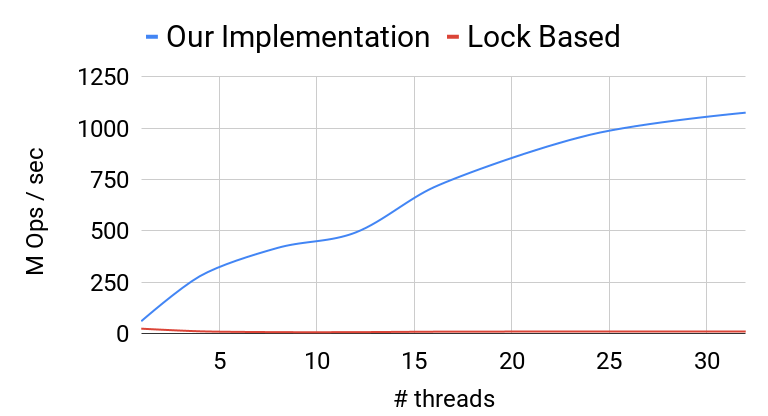
\includegraphics[width=0.39\textwidth]{images/concurrentThetaGraph.png}
  \end{center}
  \caption{Scalability of DataSketches' $\Theta$ sketch 
   protected by a lock vs. our concurrent implementation.}
  \label{fig:performance}
\end{figure}


We present a generic approach to parallelising data sketches efficiently while bounding the error that such a 
parallelisation might introduce. Our goal is to enable simultaneous queries and updates to a sketch from 
multiple  threads. Our solution is carefully designed to do so without slowing down operations as a result of synchronisation.
This is particularly challenging because sketch libraries are extremely fast, often processing tens of millions of updates per second. 

We capitalise on the well-known sketch \emph{mergeability} property~\cite{Cormode:2017}, which enables computing a sketch 
over a stream by merging sketches over substreams. Previous works have exploited this property for distributed 
stream processing (e.g.,~\cite{GoogleHLL:2013, cormode2011algorithms}), devising solutions with a sequential bottleneck at the merge phase and where queries cannot
be served before all updates complete. 
In contrast, our method is based on shared memory and constantly propagates results to a queryable sketch.
We adaptively parallelise  stream processing:  
for small streams, we forgo parallel ingestion as it might introduce significant errors;  
but as the stream becomes large, we process it in parallel using small
thread-local sketches with continuous background propagation of local results to the common (queryable) sketch.

We instantiate our generic algorithm with two popular sketches from the open-source Apache DataSketches 
(Incubating) library~\cite{DataSketches}:  
(1) a KMV $\Theta$ sketch~\cite{KMV}, which estimates the number of unique elements in a stream;
and (2) a Quantiles sketch~\cite{Agarwal:2012} estimating the stream element with a given rank. 
We have contributed the former back to the Apache DataSketches (Incubating) library~\cite{ConcurrentThetaImp}. 
Yet we emphasize that our design is generic and applicable to additional sketches. 

Figure~\ref{fig:performance} compares
the ingestion throughput of our concurrent $\Theta$ sketch to that of a lock-protected sequential sketch,
on multi-core hardware. As expected, the trivial solution does not scale whereas our algorithm scales linearly. 

Concurrency induces an error, and one of the main challenges we address is analysing this additional error.
To begin with, our concurrent sketch is a concurrent data structure, and 
we need to specify its  semantics. We do so using a flavour of 
%\emph{relaxed consistency} due to Henzinger et al.~\cite{Henzinger}    
\emph{relaxed consistency} similar to~\cite{Henzinger, alistarh2018distributionally}    
%specifically, a restricted form of their   \emph{out-of-order} relaxation 
that allows operations to ``overtake'' some other operations.  
Thus, a query may return a result that reflects all but a bounded number of the updates
that precede it. 
While relaxed semantics were previously used for data structures such as stacks~\cite{Henzinger}
and priority queues~\cite{alistarh, rihani2014multiqueues}, we believe that they are a natural fit for data sketches. 
This is because sketches are typically used to summarise streams that  arise from multiple real-world sources  
and are collected over a network with variable delays, and so even if the sketch ensures strict semantics, 
queries might miss some real-world events that occur before them. Additionally, sketches are inherently approximate.
Relaxing their semantics therefore ``makes sense'', as long as it does not excessively increase the expected error.
%Add that the error is addative and not multplicative
If a stream is much longer than the relaxation bound, then indeed the error induced by the relaxation is negligible. But since the error allowed by such
a relaxation is additive, in small streams it may have a large impact. This motivates our adaptive solution, which forgoes relaxing small streams. 

% correctness roadmap: derandomize,  strong serializability, Adversary model,

We proceed to show that our algorithm satisfies relaxed consistency. 
But this raises a new difficulty: 
relaxed consistency is defined with regards to a deterministic specification, whereas sketches are randomised.
We therefore first de-randomise the sketch's behaviour
by delegating the random coin flips to an oracle. We can then relax the resulting sequential specification.
Next, because our concurrent sketch is used within randomised algorithms, 
it is not enough to prove its linearisability. Rather, 
we prove that our generic concurrent algorithm instantiated with sequential sketch $S$
satisfies \emph{strong linearisability}~\cite{Wojciech} with regards to a relaxed sequential specification of the de-randomised $S$.
 

We then analyse the error of the relaxed sketches under random coin flips, with an adversarial scheduler that may delay operations in a
way that maximises the error. We show that our concurrent $\Theta$ sketch's error is coarsely bounded by twice
that of the corresponding sequential sketch. The error of the concurrent Quantiles sketch approaches
that of the sequential one as the stream size tends to infinity.

\vspace{-5pt}
\paragraph{Main contribution} In summary, this paper tackles the problem of concurrent sketches,
offers a general efficient solution for it, and rigorously analyses this solution. While the
paper makes use of many known techniques, it combines them in a novel way.
%we are not aware
%of any previous application of relaxed consistency to randomised statistical algorithms.
%\inred{ We discuss the difficulty of maintaining a bounded error for small streams, and show that this can be overcome without taking away from the overall performance.}
The main technical challenges we address are (1) devising a high-performance generic algorithm 
that supports real-time queries concurrently with updates without inducing an excessive error; 
(2) proving the relaxed consistency of the algorithm; 
and (3) bounding the error induced by the relaxation in both short and long streams.

The paper proceeds as follows:
Section~\ref{sec:model} lays out the model for our work and Section~\ref{sec:background} provides background
on sequential sketches. In Section~\ref{sec:concurrentSketches} we formulate a flavour of relaxed semantics
appropriate for data sketches. Section~\ref{sec:genericAlg} presents our generic algorithm, and
Section~\ref{sec:error-bounds} analyses error bounds. Section~\ref{sec:eval} empirically studies the $\Theta$ sketch's performance
and error with different stream sizes. Finally, Section~\ref{sec:discussion}
concludes. The full paper~\cite{rinberg2019fast}
%The supplementary material
formally proves strong linearisability of our generic algorithm, and
includes some of the mathematical derivations used in our analysis.

\section{Model}
\label{sec:model}

We consider a non-sequentially consistent shared memory model that enforces program order on all variables and allows
definition of \emph{atomic} variables as in Java~\cite{JavaMemoryModel} and C++~\cite{CppConcurrentMemoryModel}.
Practically speaking, reads and writes of atomic variables are guarded by memory fences, which guarantee
that all writes executed before a write {\sc w} to an atomic variable are visible to all
reads that follow (on any thread) a read {\sc r} of the same atomic variable s.t.\ {\sc r} occurs after {\sc w}. 

A thread takes \emph{steps} according to a deterministic \emph{algorithm} defined as a state machine. 
%Every step is a 3-tuple  $\left\langle state, action, state' \right\rangle$ where \emph{action} is defined by the thread's state machine.
An \emph{execution} of an algorithm is an alternating sequence of steps and states, 
where  each step follows some thread's state machine.
Algorithms implement objects supporting \emph{operations}, such as query and update. 
An operation's execution consists of a series of steps, beginning with an \emph{invoke} and ending in a \emph{response}. 
The \emph{history} of an execution $\sigma$, denoted ${\mathcal{H}}(\sigma)$, 
is its subsequence of operation invoke and response steps.
In a \emph{sequential history}, each invocation is immediately followed by its response.
The \emph{sequential specification (SeqSpec)} of an object is its set of allowed sequential histories.

%Correctness of concurrent algorithms is typically formulated using the notion of
%linearisability~\cite{herlihy1990linearizability}: 
A \emph{linearisation} of a concurrent execution $\sigma$ is a history $H \in$\emph{SeqSpec}
such that (1) after adding responses to some pending invocations in $\sigma$ and removing others,
$H$ and $\sigma$ consist of the same invocations and responses (including parameters)
and (2) $H$ preserves the order between non-overlapping operations in $\sigma$.
Golab et al.~\cite{Wojciech} have shown that in order to ensure
correct behaviour of randomised algorithms under concurrency,
one has to prove \emph{strong linearisability}:

\begin{definition}[Strong linearisability]
A function $f$ mapping executions to  histories is \emph{prefix preserving} if
for every  two executions $\sigma, \sigma'$ s.t.\ $\sigma$ is a prefix of $\sigma'$,  
$f(\sigma)$ is a prefix of $f(\sigma')$.

An algorithm $A$ is a strongly linearisable implementation of an 
object $o$ if there is a prefix preserving function $f$ that maps 
every execution $\sigma$ of $A$ to a linearisation $H$ of $\sigma$.
\end{definition}

For example, executions of atomic variables are strongly linearisable.

\input{sections/background.tex}

\section{Relaxed consistency for concurrent sketches}
\label{sec:concurrentSketches}

Previous work by Alistarh et al. [10] has presented a formalisation for a randomized relaxation of an object.
The main idea is to have the parallel execution approximately simulate the object’s correct sequential behaviour, with some provided error distribution.
In their framework, one considers the parallel algorithm and bounds the probability that it induces a large error
 relative to the deterministic sequential specification.
This approach is not suitable for our analysis, since the sequential object we parallelise (namely the sketch) is
itself randomised. Thus, there are two sources of error: (1) the approximation error in the sequential sketch and
(2) the additional error induced by the parallelisation. For the former, we wish to leverage the
existing literature on analysis of sequential sketches. To bound the latter, we use a different
methodology: we first derandomise the sequential sketch by delegating its coin flips to an oracle,
and then analyse the relaxation of the (now) deterministic sketch. Finally, we leverage the sequential sketch
analysis to arrive at a distribution for the returned value of a query.


We adopt a variant of Henzinger et al.'s~\cite{Henzinger} {\emph{out-of-order}} relaxation,  
which generalises quasi-linearisabilty~\cite{afek2010quasi}.
Intuitively, this relaxation allows a query to ``miss'' a bounded number of updates that precede it.
Because a sketch is order agnostic, we further allow re-ordering of the updates ``seen'' by a query.

A relaxed property for an object $o$ is an
extension of its sequential specification to allow more behaviours.
This requires $o$ to have a sequential specification, so
we convert sketches into deterministic objects by capturing their randomness in an external oracle; 
given the oracle's output, the sketches behave deterministically.
For the $\Theta$ sketch, the oracle's output is passed as a hidden variable to $init$, where the sketch
selects the hash function. In the Quantiles sketch, a coin flip is provided with every update.
For a derandomised sketch, we refer to the set of histories arising in its sequential
executions as \emph{SeqSketch}, and use SeqSketch as its sequential specification.
We can now define our relaxed semantics:
\begin{definition}[r-relaxation]
  A sequential history $H$ is an \emph{r-relaxation} of a sequential history $H'$,
  if $H$ is comprised of all but at most $r$ of the invocations in $H'$ and their responses,
  and each invocation in $H$ is preceded by all but at most $r$ of the invocations that precede the 
  same invocation in $H'$. The \emph{r-relaxation} of SeqSketch is the set of histories
  that have r-relaxations in SeqSketch:
  
  $SeqSketch^r \triangleq $ $\{H'|\exists H\in$SeqSketch s.t. $H$ is an r-relaxation of $H'\}$.
  \label{def:r-relaxtion}
\end{definition}

Note that our formalism slightly differs from that of~\cite{Henzinger} in that we start with a serialisation $H'$ of an object’s
execution that does not meet the sequential specification and then ``fix'' it by relaxing it to a history $H$ in the sequential
specification. In other words, we relax history $H'$ by allowing up to $r$ updates to ``overtake'' every query, so the
resulting relaxation $H$ is in SeqSketch.
\begin{figure}[h]
%\begin{wrapfigure}{r}{0.4\textwidth}
    \begin{center}
      %\vspace{-0.3in}
      
\includegraphics[width=0.38\textwidth]{images/relaxationExample}
      %\vspace{-0.3in}
    \end{center}
    \caption{$H$ is a 1-relaxation of $H'$.}
    \label{fig:relaxationExample}
%\end{wrapfigure}
\end{figure}

An example is given in Figure~\ref{fig:relaxationExample}, where $H$ is a 1-relaxation of history $H'$.
Both $H$ and $H'$ are sequential, as the operations don't overlap.
%In history $H$, $op_2$ has ``overtaken'' $op_1$ to appear first.

The impact of the $r$-relaxation on the sketch's error depends on the \emph{adversary}, which may select up to 
$r$ updates to hide from every query. There exist two adversary models:   
A \emph{weak adversary} decides which $r$ operations to omit from 
every query without observing the coin flips. 
A \emph{strong adversary} may select which updates to hide after learning 
the coin flips. Neither adversary sees the protocol's internal state, however both know the algorithm
and see the input. As the strong adversary knows the coin flips, it can then extrapolate the state; the
weak adversary, on the other hand, cannot.



\section{Generic concurrent sketch algorithm}
\label{sec:genericAlg}

We now present our generic concurrent  algorithm. 
The algorithm uses, as a building block, an existing (non-parallel) sketch. 
To this end, we extend the standard sketch interface in Section~\ref{sec:composable-sketches}, 
making it usable within our generic framework.  
Our algorithm is adaptive -- it serialises ingestion in small streams and parallelises it in large ones.
For clarity of presentation, we  present in Section~\ref{sec:basic-generic-alg} the parallel phase of the algorithm, which provides relaxed semantics appropriate for large streams;  
in the full paper~\cite{rinberg2019fast}
%in the supplementary material %Section~\ref{sec:proofs}
we prove that it is strongly linearisable
with respect to an $r$-relaxation of the sequential sketch with which it is instantiated.
Section~\ref{ssec:small-streams} then discusses the adaptation for small streams.


\subsection{Composable sketches}
\label{sec:composable-sketches}

In order to be able to build upon an existing sketch \emph{S},
we first extend it to support a limited form of concurrency.
Sketches that support this extension are called \emph{composable}.

A composable sketch has to allow concurrency between merges and queries.
To this end, we add a \emph{snapshot} API that can run concurrently with merge and
obtains a queryable copy of the sketch. The sequential specification of this operation is as follows:
\begin{description}
    \item[$S$.snapshot()] returns a copy $S'$ of $S$ such that immediately after $S'$ is returned,
     $S$.query($arg$) = $S'$.query($arg$) for every possible $arg$.
\end{description}

A composable sketch needs to allow concurrency only between snapshots
and other snapshot and merge operations, and we require that such concurrent
executions be strongly linearisable. Our $\Theta$ sketch, shown below,
simply accesses an atomic variable that holds the query result. In other sketches
snapshots can be achieved efficiently by a double collect of the relevant state.

\paragraph{Pre-filtering} When multiple sketches are used in a multi-threaded algorithm,
we can optimise them by sharing ``hints'' about the processed data.
This is useful when the stream sketching function depends on the processed stream prefix.
For example, we explain below how $\Theta$ sketches sharing a common value of $\Theta$ can sample fewer updates.
Another example is reservoir sampling~\cite{vitter1985random}. To support this optimisation,
we add the following two APIs:
\begin{description}
    \item[$S$.calcHint()] returns a value $h \neq 0$ to be used as a hint.
    \item[$S$.shouldAdd($h$, $a$)] given a hint $h$, filters out updates 
    that do not affect the sketch's state.
\end{description}    
    Formally, the semantics of these APIs are defined using the notion of summary:
    (1) When a sketch is initialised, we say that its state (or simply the sketch) \emph{summarises} the empty history,
    and similarly, the empty stream; we refer to the sketch as \emph{empty}.
    (2) After we apply a sequential history 
		\[H= S.update(a_1), S.resp(a_1), \dots S.update(a_n), S.resp(a_n)\] 
    to a sketch $S$, we say that $S$ \emph{summarises} history $H$, and,
    similarly, summarises the stream $a_1, \dots ,a_n$.
    Given a sketch $S$ that summarises a stream $A$, if shouldAdd($S.calcHint()$, $a$) returns false then
    for every streams $B_1,B_2$ and sketch $S'$ that summarises $A||B_1||a||B_2$,
    $S'$ also summarises $A||B_1||B_2$.

These APIs do not need to support concurrency, and may be trivially implemented by always returning $true$.
Note that $S$.shouldAdd is a static function that does not depend on the current state of $S$.

\paragraph{Composable $\Theta$ sketch}
 
We add the three additional APIs to Algorithm~\ref{alg:composable-theta}.
The snapshot method copies $\mathit{est}$. Note that the
result of a merge is only visible after writing to est, because it is the only variable accessed by
the query. As $\mathit{est}$ is an atomic variable, the requirement on snapshot and merge is
met. To minimise the number of updates, calcHint returns $\Theta$
and shouldAdd checks if $h(a) < \Theta$, which is safe because the value of
$\Theta$ in sketch $S$ is monotonically decreasing. Therefore, if $h(a) \geq \Theta$
then $h(a)$ will never enter the \emph{sampleSet}.

\begin{algorithm}[htb]
    \small
    %\begin{multicols}{2}
    \begin{algorithmic}[1]
        %\begin{varwidth}[t]{0.9\linewidth} 
        \Vars
        \State   sampleSet, init $k$ $1$'s \Comment samples
        \State  $\Theta$, init $1$			\Comment threshold
        \State {\tt atomic} est, init $0$ \Comment estimate
        \State $h$, init random uniform hash function 
        \EndFor
        
        \Procedure{query}{arg}
        \State \Return $est$ \label{l:query}
        \EndProcedure
        
        \Procedure{update}{arg}
        \If{$h$(arg) $\geq \Theta$} \Return
        \EndIf
        \State add $h$(arg) to \emph{sampleSet}
        \State keep $k$ smallest samples in \emph{sampleSet}
        \State $\Theta \leftarrow max(sampleSet)$
        \State $\mathit{est}$ $\leftarrow $ $\left( |\text{sampleSet}|-1 \right)$ / $\Theta$
        \EndProcedure
        %\end{varwidth}\quad\quad\quad 
        %\columnbreak
        %\begin{varwidth}[t]{1\linewidth}

        \Procedure{merge}{S}
        \State sampleSet $\leftarrow$ merge sampleSet and $S$.sampleSet
        \State keep $k$ smallest values in sampleSet
        \State $\Theta \leftarrow max($sampleSet$)$
        \State $\mathit{est}$ $\leftarrow $ $\left( |\text{sampleSet}|-1 \right)$ / $\Theta$ \label{l:update-est}
        \EndProcedure
        
        \Procedure{snapshot}{}
            \State $localCopy \leftarrow empty sketch$
            \State $localCopy.\mathit{est} \leftarrow \mathit{est}$
            \State \Return $localCopy$
        \EndProcedure
    
        \Procedure{calcHint}{}
            \State \Return $\Theta$
        \EndProcedure
    
        \Procedure{shouldAdd}{H, arg}
            \State \Return $h$(arg) $< H$
        \EndProcedure
    %\end{varwidth}

    \end{algorithmic}
    %\end{multicols}
    \caption{Composable $\Theta$ sketch.}
    \label{alg:composable-theta}
\end{algorithm}

\subsection{Generic algorithm}
\label{sec:basic-generic-alg}

To simplify the presentation and proof, we first discuss an unoptimised version of
our generic concurrent algorithm (Algorithm~\ref{alg:generic-concurrent} without the gray lines)  called 
\emph{ParSketch},
and later an optimised version of the same algorithm (Algorithm~\ref{alg:generic-concurrent} including the gray lines
and excluding underscored line~\ref{l:signal}).

The algorithm is instantiated by a composable sketch and sequential sketches.
It uses multiple threads to process incoming stream elements 
and services queries at any time during the sketch's construction.
Specifically, it uses $N$ worker threads, $t_1,\dots,t_N$, each of which samples
stream elements into a local sketch $localS_i$, and a propagator thread $t_0$ that merges local sketches
into a shared composable sketch $globalS$. Although the local sketch resides in
shared memory, it is updated exclusively by its owner update thread $t_i$ and 
read exclusively by $t_0$. Moreover, updates and reads do not happen in
parallel, and so cache invalidations are minimised. The global sketch is updated only by $t_0$
and read by query threads. We allow an unbounded number of query threads. 

After $b$ updates are added to $localS_i$, $t_i$ signals to the propagator to merge
it with the shared sketch. It synchronises with $t_0$ using a 
single \emph{atomic} variable $prop_i$, which $t_i$ sets to 0.  
Because $prop_i$ is atomic, the memory model
guarantees that all preceding updates to $t_i$'s local sketch are visible to
the background thread once $prop_i$'s update is.
This signalling is relatively expensive (involving a memory fence),  
but we do it only once per $b$ items retained in the local sketch.

After signalling to $t_0$, $t_i$ waits
until $prop_i \neq 0$  (line~\ref{l:wait}); 
this indicates that the propagation has completed, and $t_i$ can 
reuse its local sketch. Thread $t_0$ piggybacks the hint \emph{H} it
obtains from the global sketch on $prop_i$,
and so there is no need for further synchronisation in order to pass the hint.

Before updating the local sketch, $t_i$ invokes shouldAdd to check
whether it needs to process \emph{a} or not. For example, the $\Theta$ sketch discards updates whose hashes are
greater than the current value of $\Theta$. The global thread passes the global sketch's
value of $\Theta$ to the update threads, pruning updates that would end up being discarded
during propagation. This significantly
reduces the frequency of propagations and associated memory fences.

\begin{algorithm}[htb]
    \small
    %\begin{multicols}{2}
    \begin{algorithmic}[1]
    \setcounter{ALG@line}{100}

    \Vars
    \State composable sketch \emph{globalS}, init empty
    \State constant $b$ \Comment relaxation is $2Nb$
    \ForEach{update thread $t_i$} , $0 \leq i \leq N$
        \State sketch \emph{localS$_i$}\ingray{[$2$]}, init empty
        \ingray{\State int \emph{cur}$_i$, init 0}
        \State int $counter_i$, init $0$
        \State int \emph{hint}$_i$, init $1$
        \State int {\tt atomic} $prop_i$, init $1$
    \EndFor
    \EndFor

    \Procedure{propagator}{}
    \While {true}
    \ForAll{thread $t_i$ s.t. $prop_i=0$}
        \State $globalS.merge(localS_i$\ingray{[1-$cur_i$]}$)$ \label{l:merge}
        \State $localS_i$\ingray{[1-$cur_i$]}$ \leftarrow $empty sketch \label{l:emptyAux}
		\State $prop_i \leftarrow globalS.calcHint()$ \label{l:calcHint}
    \EndFor
    \EndWhile
    \EndProcedure

    %\columnbreak

    \Procedure{query}{arg}
    \State $localCopy \leftarrow globalS.snapshot(localCopy)$
    \State \Return $localCopy.query(arg)$
    \EndProcedure
    
    \Procedure{update$_i$}{$a$}
    \If{$\neg$shouldAdd(\emph{hint}$_i$, $a$)} \Return \label{l:shouldAdd}
    \EndIf
    \State $counter_i \leftarrow counter_i + 1$ \label{l:countup}
    \State $localS_i$\ingray{[$cur_i$]}$.update(a)$ \label{l:update}
    \If{$counter_i = b$} \label{l:checkfull}
    \State \underline{$prop_i \leftarrow 0$} \Comment In non-optimised version\label{l:signal}
    \State wait until $prop_i \neq 0$ \label{l:wait}
    \ingray{\State $cur_i \leftarrow 1 - cur_i$} \label{opt:l:swap-local-aux}
    \State \emph{hint}$_i \leftarrow prop_i$ \label{l:updateHint}
    \State $counter_i \leftarrow 0$ \label{l:zeroCounter}
    \ingray{\State $prop_i \leftarrow 0$} \Comment In optimised version\label{opt:l:signal}
    \EndIf
    \EndProcedure

    \end{algorithmic}
    %\end{multicols}
    \caption{\ingray{Optimised} generic concurrent algorithm.}
    \label{alg:generic-concurrent}
\end{algorithm}

Query threads use the snapshot method, which can be safely run concurrently with merge,
hence there is no need to synchronise between the query threads and $t_0$. The freshness
of the query is governed by the $r$-relaxation.
In the full paper~\cite{rinberg2019fast},
%In the supplementary material Section~\ref{subsec:Generic-algorithm-proof}
we prove Lemma~\ref{lemma:genereic-strong} below, asserting that
the relaxation is $Nb$. This may seem straightforward as $Nb$ is the combined size of the
local sketches. Nevertheless, proving this is not trivial because the local sketches pre-filter
many additional updates, which, as noted above, is instrumental for performance. 

\begin{lemma}
    $ParSketch$ instantiated with $SeqSketch$ is strongly linearisable with regards to $SeqSketch^{Nb}$.
    \label{lemma:genereic-strong}
\end{lemma}


A limitation of \emph{ParSketch} is that update threads are idle while waiting for the propagator to execute the merge. This
may be inefficient, especially if a single propagator iterates through many local sketches.
Algorithm~\ref{alg:generic-concurrent} with the gray lines included and the underlined line omitted presents
the optimised \emph{OptParSketch} algorithm, which improves thread utilisation via
double buffering.

In \emph{OptParSketch}, $localS_i$ is an array of two sketches. When $t_i$ is ready to propogate $localS_i[cur_i]$, it
flips the $cur_i$ bit denoting which sketch it is currently working on (line~\ref{opt:l:swap-local-aux}), 
and immediately sets $prop_i$ to 0 (line~\ref{opt:l:signal}) in order to allow the propagator to
take the information from the other one. It then starts digesting updates in a fresh sketch.

In the full paper~\cite{rinberg2019fast}
%In the supplementary material Section~\ref{subsec:Optimised-algorithm-proof}
we prove the correctness of the optimised
algorithm by simulating $N$ threads of \emph{OptParSketch}
using $2N$ threads running \emph{ParSketch}. We do this by showing
a \emph{simulation relation}~\cite{lynch1996distributed}. We use forward simulation (with
no prophecy variables), ensuring strong linearisability. We conclude the following theorem:
\begin{restatable}{rthm}{optgenereicstrong}
    \emph{OptParSketch} instantiated with $SeqSketch$ is strongly linearisable with regards to \emph{SeqSketch}$^{2Nb}$.
    \label{lemma:opt-genereic-strong}
\end{restatable}

\subsection{Adapting to small streams}
\label{ssec:small-streams}

By Theorem~\ref{lemma:opt-genereic-strong}, a query can miss up to $r$ updates. For small
streams, the error induced by this can be very large.
For example, the sequential $\Theta$ sketch answers queries with perfect accuracy in streams with
up to $k$ unique elements, but if $k<r$, the relaxation can miss \emph{all} updates.
In other words, while the additive error is guaranteed to be bounded by $r$, the relative 
error can be infinite.  

To rectify this, we implement \emph{eager propagation} for small streams, 
whereby update threads propagate updates immediately to the shared sketch 
instead of buffering them. 
% and the shared sketch is accessed sequentially (protected by a lock or CAS).  
Note that during the eager phase, updates are processed sequentially. 
Support for eager propagation can be added to Algorithm~\ref{alg:generic-concurrent} 
by initialising $b$ to $1$ and having the propagator thread raise it to the
desired buffer size once the stream exceeds some pre-defined length. 
The error analysis of the next section can be used to determine the adaptation point.


\section{Deriving error bounds}
\label{sec:error-bounds}
%We bound the error induced by relaxation on two representative sketches.
Section~\ref{ssec:theta-analysis} discusses the error introduced to the
expected estimation and RSE of the KMV $\Theta$ sketch.
Section~\ref{ssec:quantiles-error-analysis} analyses the PAC Quantiles sketch.
The full paper~\cite{rinberg2019fast} contains mathematical derivations used throughout this section. 

\subsection{$\Theta$ error bounds}
\label{ssec:theta-analysis}

We bound the error introduced by an $r$-relaxation of the $\Theta$ sketch. Given
Theorem~\ref{lemma:opt-genereic-strong}, the optimised concurrent sketch's error is bounded
by the relaxation's error bound for $r=2N$$b$. We consider strong and weak adversaries,
${\mathcal{A}}_s$ and ${\mathcal{A}}_w$, resp. For the strong adversary we are able to show only numerical
results, whereas for the weak one we show closed-form bounds. The results are summarised in Table~\ref{table:Theta-Error-Summary}.
Our analysis relies on known results from order statistics~\cite{david2004order}.
It focuses on long streams, and assumes $n>k+r$.

%\begin{table}[H]
%    \begin{tabular}{c|cc|cc|cc}
%                      & \multicolumn{2}{c|}{Sequential sketch} & \multicolumn{2}{c|}{Strong adversary ${\mathcal{A}}_s$} & \multicolumn{2}{c}{Weak adversary ${\mathcal{A}}_w$}   \\[5pt]
%                      & Closed-form& Numerical& \multicolumn{2}{c|}{Numerical} & \multicolumn{2}{c}{Closed-form}   \\[5pt]
%                      \hline
%    Expectation & $n$        & $2^{15}$        & \multicolumn{2}{c|}{$2^{15} \cdot 0.995$}          & \multicolumn{2}{c}{$n\frac{k-1}{k+r-1}$} \\[5pt]
%    RSE & $\leq \frac{1}{\sqrt{k-2}}$        & $\leq 3.1\%$        & \multicolumn{2}{c|}{$\leq 3.8\%$}           & \multicolumn{2}{c}{$\leq 2\frac{1}{\sqrt{k-2}}$}         
%    \end{tabular}
%    \caption{Analysis of $\Theta$ sketch with numerical values for $r=8, k=2^{10}, n=2^{15}$.}
%    \label{table:Theta-Error-Summary}
%\end{table}

\begin{table*}[!ht]
    % Table content (and caption)
    \begin{tabular}{c|cc|cc|cc}
        & \multicolumn{2}{c|}{Sequential sketch} & \multicolumn{2}{c|}{Strong adversary ${\mathcal{A}}_s$} & \multicolumn{2}{c}{Weak adversary ${\mathcal{A}}_w$}   \\%[5pt]
        & Closed-form& Numerical& \multicolumn{2}{c|}{Numerical} & \multicolumn{2}{c}{Closed-form}   \\%[5pt]
        \hline
        Expectation & $n$        & $2^{15}$        & \multicolumn{2}{c|}{$2^{15} \cdot 0.995$}          & \multicolumn{2}{c}{$n\frac{k-1}{k+r-1}$} \\%[5pt]
        RSE & $\leq \frac{1}{\sqrt{k-2}}$        & $\leq 3.1\%$        & \multicolumn{2}{c|}{$\leq 3.8\%$}           & \multicolumn{2}{c}{$\leq 2\frac{1}{\sqrt{k-2}}$}         
    \end{tabular}
    \caption{Analysis of $\Theta$ sketch with numerical values for $r=8, k=2^{10}, n=2^{15}$.}
    \label{table:Theta-Error-Summary}
\end{table*}

We would like to analyse the distribution of the $k^{th}$ largest element in the 
stream that the relaxed sketch processes, as this determines the result returned by the algorithm. 
We cannot use order statistics to analyse this 
because the adversary alters the stream and so the stream seen by the algorithm is not random.
%the $k^{th}$ largest element in the stream is not a random variable. 
However, the stream of hashed unique elements seen by the adversary \emph{is} random. 
Furthermore, if the adversary hides from the algorithm $j$ elements 
smaller than $\Theta$, then the $k^{th}$ largest element in the stream seen
by the  sketch is the $(k+j)^{th}$ largest element in the original stream seen by the adversary. 
This element is a random variable and therefore we can apply order statistics to it.  

We thus model the hashed unique elements in the stream $A$ processed before a given
query as a set of $n$ labelled iid random variables $A_1,\dots,A_n$, taken uniformly 
from the interval $[0,1]$. Note that
$A$ is the stream observed by the reference sequential sketch, and 
also by adversary that hides up to $r$ elements from the relaxed sketch. 
Let $M_{(i)}$ be the $i^{th}$ minimum value among the $n$ random variables $A_1,\dots,A_n$.

Let $est(x) \triangleq \frac{k-1}{x}$ be the estimate computation
with a given $x=\Theta$ (line~\ref{l:update-est} of Algorithm~\ref{alg:composable-theta}).
The sequential (non-relaxed) sketch returns $e=est(M_{(k)})$.
It has been shown that the sketch is unbiased~\cite{KMV}, i.e., $E[e]=n$ the number of unique elements,
and $RSE[e]\leq \frac{1}{\sqrt{k-2}}$.
The \emph{Relative Standard Mean Error (RSME)} is the error relative to the mean, formally defined in
the full paper~\cite{rinberg2019fast}.
%the supplementary material Section~\ref{ssec:RSE-RMSE}.
Because this sketch is unbiased, \emph{RSE}$[e]=$\emph{RSME}$[e]$.


In a relaxed history, the adversary chooses up to $r$ variables to hide from the given query so as to maximise its
error. It can also re-order elements, but the state of a $\Theta$ sketch after a set of updates
is independent of their processing order. Let $M^r_{(i)}$ be the $i^{th}$ minimum value among
the hashes seen by the query, i.e., arising in updates that precede the query in the relaxed history.
The value of $\Theta$ is $M^r_{(k)}$, which is equal to $M_{(k+j)}$ for some $0 \leq j \leq r$.
We do not know if the adversary can actually control $j$,
but we know that it can impact it, %and so to bound the error, we can take the worst possible $j$.
%While an arbitrary set of $r$ updates is hidden, in the $\Theta$ sketch,
%only hidden elements that impact $j$ (have hashes smaller than $M^r_{(k)}$)
%affect the query.
and so for our error analysis, we consider strictly stronger adversaries --
we allow both the weak and the strong adversaries to choose the number of hidden
elements $j$. Our error analysis gives an upper bound on the error induced by our adversaries.
Note that the strong adversary can choose $j$ based on the coin flips,
while the weak adversary cannot, and therefore chooses the same $j$ in all runs.
%The strong adversary knows the hash function and can select $j$ adaptively; the
%weak adversary does not and therefore chooses the same $j$ in all runs.  
%Note that $j$ counts only hidden elements smaller
%than $\Theta$; others are inconsequential.
In the full paper~\cite{rinberg2019fast} we show that
the largest error is always obtained either for $j=0$ or for $j=r$. 
\begin{figure}[b]
%\begin{wrapfigure}{r}{0.4\textwidth}
    \begin{center}
        %\vspace{-0.4in}
        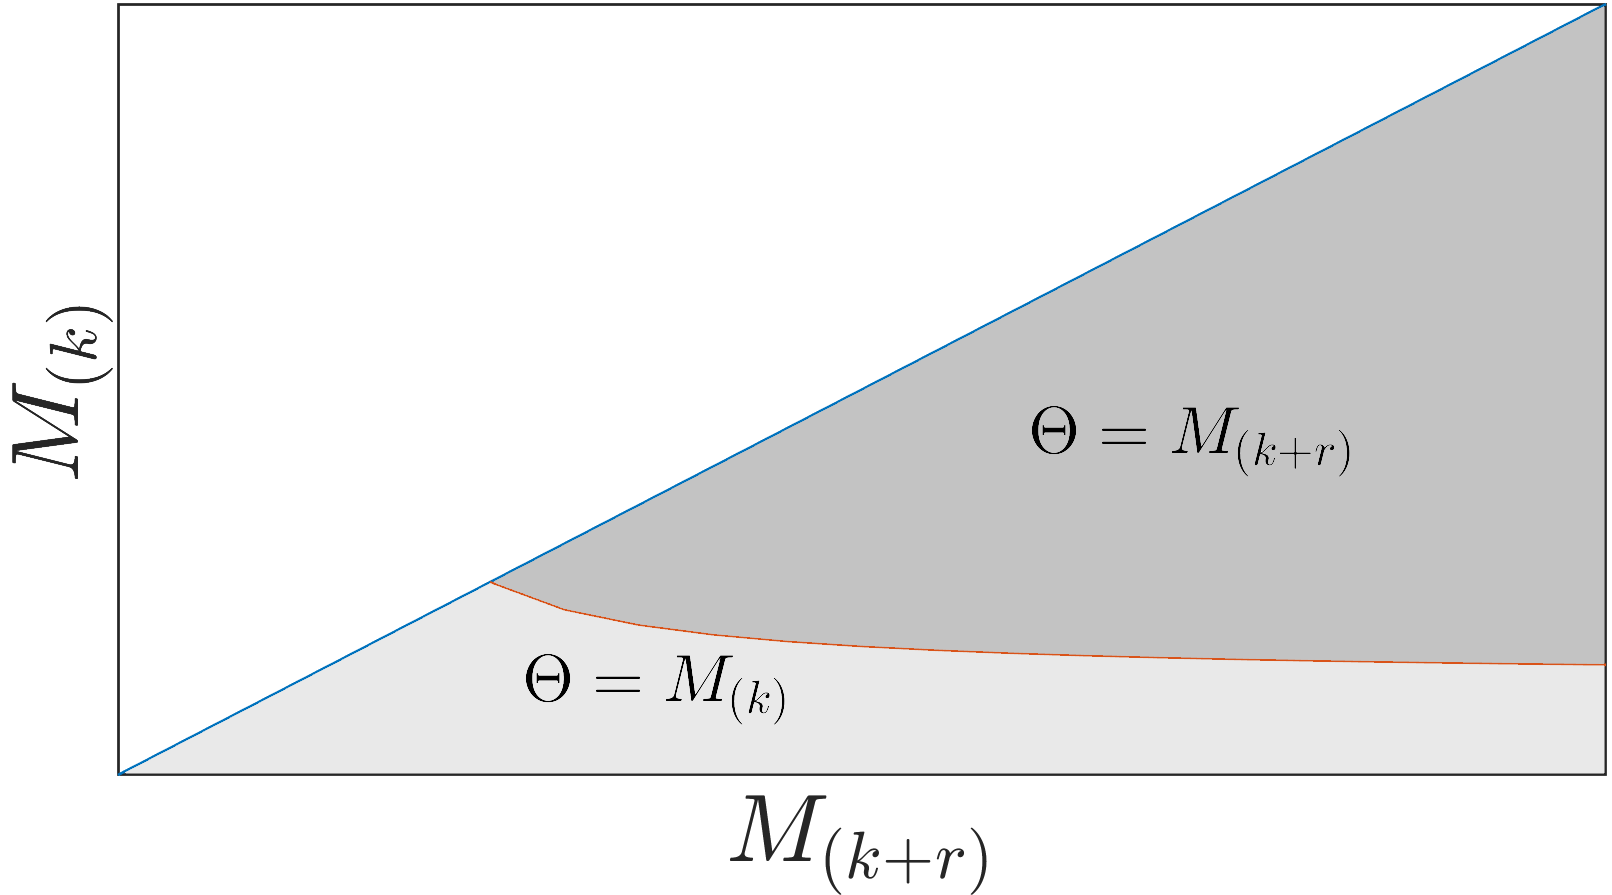
\includegraphics[width=0.38\textwidth]{images/areaGraph.png}
        %\vspace{-0.2in}
    \end{center}
    \caption{Areas of $M_{(k)}$ and $M_{(k+r)}$. In the dark gray 
    ${\mathcal{A}}_s$ induces $\Theta=M_{(k+r)}$, and in the light gray, $\Theta=M_{(k)}$. The white
    area is not feasible.} %\vspace{-0.1in}
    \label{fig:areaGraph}
%\end{wrapfigure}
\end{figure}

Given an adversary $\mathcal{A}$ that induces an approximation $e_{\mathcal{A}}$, in the full paper~\cite{rinberg2019fast} we prove
the following bound:
%Lemma~\ref{lemma:theta-adversary-bound} in the supplementary material Section~\ref{ssec:theta-error-bounds} proves the following bound:
\begin{align*}
    \text{RSE}[e_{\mathcal{A}}] \leq \sqrt{\frac{\sigma^2(e_{\mathcal{A}})}{n^2}} + \sqrt{\frac{(E[e_{\mathcal{A}}] - n)^2}{n^2}}.
\end{align*}

\paragraph{Strong adversary ${\mathcal{A}}_s$} The strong adversary knows the coin flips in advance, and thus chooses
$j$ to be $g(0, r)$, where $g$ is the
choice that maximises the error:
\begin{align*}
    g(j_1, j_2) \triangleq \argmax_{j \in \left\{j_1, j_2\right\}} \abs{\frac{k-1}{M_{(k+j)}} - n}.
\end{align*} 

\begin{figure}[b]
%\begin{wrapfigure}{l}{0.4\textwidth}
    \begin{center}
        %\vspace{-0.2in}
        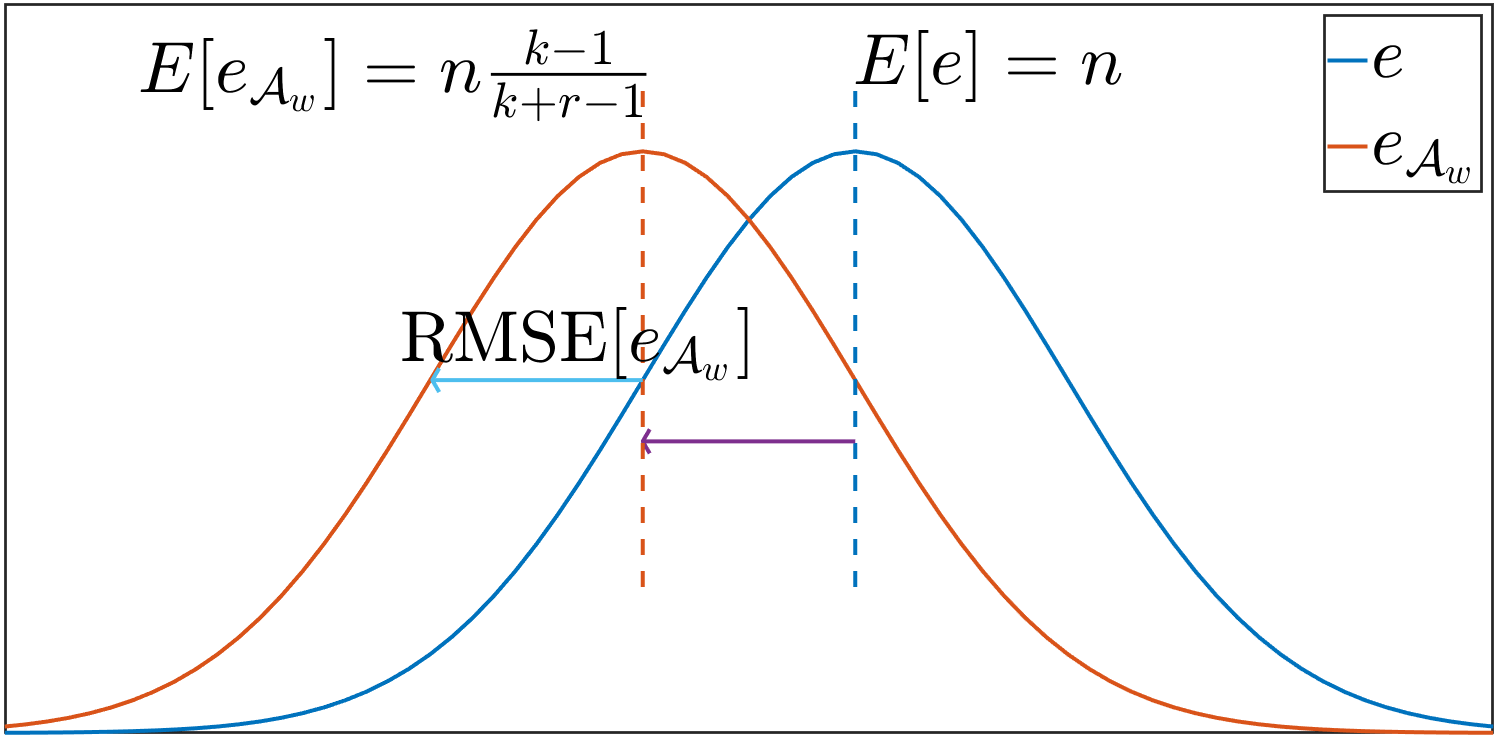
\includegraphics[width=0.39\textwidth]{images/thetaGraph.png}
        %\vspace{-0.2in}
    \end{center}
    \caption{Distribution of estimators $e$ and $e_{{\mathcal{A}}_w}$. The RSE of $e_{{\mathcal{A}}_w}$ with regards to $n$ is bounded
    by the relative bias plus the RMSE of $e_{{\mathcal{A}}_w}$.}%\vspace{-0.2in}}
    \label{fig:thetaGraph}
%\end{wrapfigure}
\end{figure}

In Figure~\ref{fig:areaGraph} we plot the regions where $g$ equals $0$
and $g$ equals $r$, based on their possible combinations of values. The estimate
induced by ${\mathcal{A}}_s$ is $e_{{\mathcal{A}}_s} \triangleq \frac{k-1}{M_{(k+g(0,r))}}$. The expectation
and standard error of $e_{{\mathcal{A}}_s}$ are calculated by integrating over the gray areas
in Figure~\ref{fig:areaGraph}
using their joint probability function from order statistics. In the full paper~\cite{rinberg2019fast} we give
%Equations \ref{eq:strong-expectation}
%and \ref{eq:strong-se-bound} in the supplementary material Section~\ref{ssec:theta-error-bounds} give
the formulas for the expected estimate and its RSE bound, resp. We do not have
closed-form bounds for these equations. Example numerical results are
shown in Table~\ref{table:Theta-Error-Summary}.

\paragraph{Weak adversary ${\mathcal{A}}_w$} Not knowing the coin flips, ${\mathcal{A}}_w$ chooses $j$
that maximises the expected error for a random hash function:
$E[n-est(M^r_{(k)})]=E[n-est(M_{(k+j)})]=n-n\frac{k-1}{k+j-1}$. Obviously this
is maximised for $j=r$. The orange curve in Figure~\ref{fig:thetaGraph} depicts
the distribution of $e_{{\mathcal{A}}_w}$, and the distribution of $e$ is shown in blue.

%Not knowing the coin flips, what ${\mathcal{A}}_w$ will
%attempt to maximise the expected error of the query \inred{by doing what?}:
%\begin{align*}
%    E[n-est(M^r_{(k)})]=E[n-est(M_{(k+j)})]=n-n\frac{k-1}{k+j-1}
%\end{align*}

%For some $0 \leq j \leq r$. Note that the error is maximised for $j=r$.
%As the adversary does not know the coin flips, it will attempt
%to maximise the number of updates stuck in the local buffers, as an
%update in the local buffers has a hash value is lower than $\Theta$ (or rather lower than $\Theta$
%after the last propagation). We can therefore bound the error induced by this adversary by an
%adversary $\hat{{\mathcal{A}}}_w$ that always hides $r$ elements smaller than $\Theta$, thus forcing
%$M^r_{(k)}=M_{(k+r)}$. The orange curve in Figure~\ref{fig:thetaGraph} depicts
%the distribution of $e_{\hat{{\mathcal{A}}}_w}$, and the distribution of $e$ is shown in blue.

In the full paper~\cite{rinberg2019fast},
%In Equation~\ref{eq:theta-rse-weak-bound} in the supplementary material Section~\ref{ssec:theta-error-bounds} 
we show that the RSE
is bounded by $\sqrt{\frac{1}{k-2}} + \frac{r}{k-2}$ for $\hat{{\mathcal{A}}}_w$, and therefore so
is that of ${\mathcal{A}}_w$.
Thus, whenever $r$ is at most $\sqrt{k-2}$, the RSE of the relaxed
$\Theta$ sketch is coarsely bounded by
twice that of the sequential one. And in case $k \gg r$, the addition to the $RSE$ is negligible.

\subsection{Quantiles error bounds}
\label{ssec:quantiles-error-analysis}

%\begin{wraptable}{c}{0pt}
%    \begin{tabular}{c|ccc}
%    Quantile        & Sequential                                   & Weak adversary ${\mathcal{A}}_w$ \\[5pt]
%    \hline
%    $\phi \leq 0.5$ & $\phi n \pm \epsilon n$ & $\phi n + (1-\phi)r \pm \epsilon(n - r)$ \\[5pt]
%    $\phi > 0.5$    & $\phi n \pm \epsilon n$ & $\phi n -\phi r \pm \epsilon(n - r)$
%    \end{tabular}
%    \caption{Quantiles sketch: Result range with probability $1-\delta$, for sequential sketch and $r$-relaxation with weak adversary,
%    and $\epsilon_r=\epsilon - \frac{r \epsilon}{n} + \frac{r}{n}$.}
%    \label{table:Quantiles-Error-Summary}
%\end{wraptable}

\iffalse
\begin{wraptable}{c}{0pt}
    \begin{tabular}{c|ccc}
    Quantile        & Sequential                                   & Weak adversary ${\mathcal{A}}_w$ \\[5pt]
    \hline
    $\phi $ & $\phi n \pm \epsilon n$ & $\phi n \pm \left(\epsilon - \frac{r \epsilon}{n} + \frac{r}{n}\right) n$ 
    \end{tabular}
    \caption{Quantiles sketch: Result range with probability $1-\delta$, for sequential sketch and $r$-relaxation with weak adversary,
    and $\epsilon_r=\epsilon - \frac{r \epsilon}{n} + \frac{r}{n}$.}
    \label{table:Quantiles-Error-Summary}
\end{wraptable}
\fi

We now analyse the error for any implementation of the sequential Quantiles sketch, provided that the sketch is
\emph{PAC}, meaning that a query for quantile $\phi$
returns an element whose rank is between $(\phi-\epsilon)n$ and $(\phi+\epsilon)n$ with 
probability at least $1-\delta$ for some parameters $\epsilon$ and $\delta$. We show that the $r$-relaxation of
such a sketch returns an element whose rank is in the range $(\phi \pm\epsilon_r)n$ with probability at
least $1-\delta$ for $\epsilon_r=\epsilon - \frac{r \epsilon}{n} + \frac{r}{n}$.

%The results are summarised in Table~\ref{table:Quantiles-Error-Summary}.

Although the desired summary is order agnostic here too, Quantiles sketch implementations (e.g., \cite{Agarwal:2012})
are sensitive to the processing order. In this case, advanced knowledge of the coin flips can increase the error
already in the sequential sketch. Therefore, we do not consider a strong adversary, but rather discuss only the weak one.
Note that the weak adversary attempts to maximise $\epsilon_r$.

Consider an adversary that knows $\phi$ and chooses to hide
$i$ elements below the $\phi$ quantile and $j$ elements above it, such that $0\leq i+j\leq r$. The rank of the element
returned by the query among the $n-(i+j)$ remaining elements is in the range 
$\phi(n-(i+j)) \pm \epsilon(n-(i+j))$.
There are $i$ elements below this quantile that are missed, and therefore its rank in the original stream is in the range:
\begin{equation}
    \left[ (\phi-\epsilon)(n-(i+j)) + i , (\phi+\epsilon)(n-(i+j)) + i \right].
    \label{eq:rank-range}
\end{equation}

This can be rewritten as:
\begin{equation}
\begin{split}
    [\phi n - (\phi j - (1-\phi)i+\epsilon(n-(i+j))), \\
    \phi n + ((1-\phi)i - \phi j +\epsilon(n-(i+j))) ] 
\end{split}
    \label{eq:rank-range-2}
\end{equation}

\iffalse

\begin{wrapfigure}{r}{0.3\textwidth}
    \begin{center}
        %\vspace{-0.2in}
      
\includegraphics[width=0.29\textwidth]{images/quantilesRelaxtionRanges.png}
      %\vspace{-0.2in}
    \end{center}
    \caption{Ranges where the result of a query($\phi$) to
        a Quantiles sketch resides with probability $1-\delta$;
        for a sequential sketch and an $r$-relaxation. \vspace{0.2in}}
    \label{fig:quantiles-range}
\end{wrapfigure}

Note that this interval is symmetric around $\phi(n-(i+j)) + i$.
The adversary attempts to maximise the distance of the edges of this interval from the true rank,
(i.e., maximise $\epsilon_r$). The distance between the central points is:
\begin{align*}
    \abs{\phi n + (1-\phi)i - \phi j - \phi n}=\abs{(1-\phi)i - (\phi)j}.
\end{align*}
Given that $0\leq i+j\leq r$, we show that this expression is maximised
for $i+j=r$.
This is proven in the full paper~\cite{rinberg2019fast}.
%This is proven in Claim~\ref{claim:sum-r} in the supplementary material Section~\ref{ssec:quantiles-sketch-error-bounds}.
By substituting $j=r-i$ into the error formula, we get:
\begin{align*}
    \abs{(1-\phi)i - (\phi)(r-i)}=\abs{i - \phi r}.
\end{align*}
As $0\leq \phi \leq 1$, the following claim follows immediately:
\begin{claim}
    For $\phi \leq 0.5$ the adversary maximises the distance by choosing $i=r$ (and therefore $j=0$)
    and for $\phi > 0.5$ the adversary maximises the error by choosing $i=0$ (and therefore $j=r$).
    \label{clm:quantiles-relaxation-choice}
\end{claim}

\fi
In the full paper~\cite{rinberg2019fast}, we
%In Lemma~\ref{lemma:quantiles-weak-adversary} in the supplementary material Section~\ref{sec:appendix-error-bounds} we
show that the $r$-relaxed sketch returns an element whose rank is
between $(\phi-\epsilon_r)n$ and $(\phi+\epsilon_r)n$ with probability at
least $1-\delta$, where $\epsilon_r=\epsilon - \frac{r \epsilon}{n} + \frac{r}{n}$. Thus
the impact of the relaxation diminishes as $n$ grows.
%The ranges are illustrated in Figure~\ref{fig:quantiles-range}.

\section{$\Theta$ sketch evaluation}
\label{sec:eval}

This section presents an evaluation of an implementation of our algorithm for the $\Theta$ sketch.
Section~\ref{ssec:setup-and-methodology} presents the methodology for the analysis.
Section~\ref{ssec:results} shows the results under different
workloads and scenarios. Finally, Section~\ref{ssec:tradeoffs} discusses the tradeoff between
accuracy and throughput.

\subsection{Setup and methodology}
\label{ssec:setup-and-methodology}

Our implementation~\cite{ConcurrentThetaImp} extends the code in Apache DataSketches (Incubating)~\cite{DataSketches}, a Java
open-source library of stochastic streaming algorithms. The $\Theta$ sketch there differs slightly
from the KMV $\Theta$ sketch we used as a running example, and is based on a HeapQuickSelectSketch family.
In this version, the sketch stores between $k$ and $2k$ items, whilst keeping $\Theta$ as the $k^{\text{th}}$
largest value. When the sketch is full, it is sorted and the largest $k$ values are discarded.

Concurrent $\Theta$ sketch is generally available in the Apache DataSketches (Incubating)
library since V0.13.0. The sequential implementation and the sketch at the core of the global sketch
in the concurrent implementation are the both \\ HeapQuickSelectSketch, which is the default sketch family.

As explained in Section~\ref{ssec:small-streams}, we implement a limit for eager propagation as a function
of the configurable error parameter $e$; the function we use is $2 / e^2$. The local sketches define $b$
as a function of $k$, $e$, and $N$ (the number of writer threads). The error induced by the relaxation
does not exceed $e$, and thus the total error is bounded by $\max\{e + \frac{1}{\sqrt{k}}, \frac{2}{\sqrt{k}}\}$.

Eager propagation, as described in the pseudo-code, requires context switches incurring a high overhead. In the
implementation, either the local thread itself executes every update to the global sketch (equivalent to a
buffer size of 1) or lazily delegates updates to a background thread. While the sketch is in eager propagation
mode, the global sketch is protected by a shared boolean flag. When the sketch switches to estimate mode it
is guaranteed that no eager propagation gets through; instead local threads pass the buffer via lazy propagation.
This implementation ensures that: (a) local threads avoid costly context switches when the sketch is small, and (b)
lazy propagation by a background thread is done without synchronisation.

Unless otherwise stated, sketches are configured with $k=4096$, and $e=0.04$; thus the exact limit
is $2/e^2=1250$, and $b$ is set (by the implementation) to a value between $1$ and $5$ to accommodate the
error bound. Our first set of tests run on a 12-core Intel Xeon E5-2620 machine -- this machine is similar
to that which is used by production servers. For the scalability evaluation (shown in the introduction) we use a 32-core Intel Xeon
E5-4650 to get a large number of threads. Both machines have hyper-threading disabled, as it introduces
non-monotonic effects among threads sharing a core.

We focus on two workloads: (1) write-only -- updating a sketch with a stream of unique values; (2) mixed
read-write workload -- updating a sketch with background reads querying the number of unique values in
the stream. Background reads refer to dedicated threads that occasionally (with $1$ms pauses) execute a query.
These workloads were chosen to simulate read-world scenarios where updates are constantly streaming from
a feed or multiple feeds, while queries arrive at a lower rate.

To run the experiments we employ a multi-thread extension of the characterization
framework. This is the Apache DataSketch evaluation benchmark suite, which measures
both the speed and accuracy of the sketch. 

For measuring write throughput, the sketch is fed with a continuous data stream. The size of
the stream varies from 1 to 8M unique values. For each size $x$ we measure the time $t$ it takes to feed the
sketch $x$ unique values, and present it in term of throughput ($x/t$). To minimise measurement noise,
each point on the graph represents an average of many trials. The number of trials is very high
($2^{18}$) for points at the low end of the graph. It gradually decreases as the size of the
sketch increases. At the high end (at 8M values per trial) the number of trials is 16. This is because
smaller stream sizes tend to suffer more from measurement noise.

The accuracy of a concurrent $\Theta$ sketch is measured only in a single-thread environment. As
in the performance evaluations, the $x$-axis represents the number of unique values fed into the sketch
by a single writing thread. For each size $x$, one trial logs the estimation result after feeding $x$
unique values to the sketch. In addition, it logs the Relative Error (RE) of the estimate, where
$\mathit{RE} = \mathit{MeasuredValue}/\mathit{TrueValue} - 1$. This trial is repeated 4K times,
logging all estimation and $\mathit{RE}$ results. The curves depict the mean and some
quantiles of the distributions of error measured at each $x$-axis point on the graph, including the median. 
This type of graph is called a ``pitchfork''.


\subsection{Results}
\label{ssec:results}

\paragraph{Accuracy results}
Our first set of tests runs on a 12-core Intel Xeon E5-2620 machine. The accuracy results for the concurrent $\Theta$ sketch
without eager propagation are presented in Figure~\ref{fig:accuracy}. There are two interesting phenomena worth noting.
First, it is interesting to see empirical evaluation reflecting the theoretical analysis presented in Section~\ref{ssec:theta-analysis},
where the pitchfork is distorted towards underestimating the number of unique values. Specifically, the mean relative error is smaller
than $0$ (showing a tendency towards underestimating), and the relative error in all measured quantiles tends to be smaller
than the relative error of the sequential implementation.

Second, when the stream size is less than $2k$, $\Theta=1$ and the estimation is the number of values propagated to the
global sketch. If we forgo eager propagation, the number of values in the global sketch depends on the delay in propagation. The
smaller the sketch, the more significant the impact of the delay, and the mean error reaches as high as $94\%$ (the error in
the figure is capped at $10\%$). As the number of propagated values approaches $2k$, the delay in propagation is less significant, and
the mean error decreases. This excessive error is remedied by the eager propagation mechanism. The maximum error allowed by
the system is passed as a parameter to the concurrent sketch, and the global sketch uses eager propagation to stay within
the allowed error limit. Figure~\ref{fig:accuracy-adaptive} depicts the accuracy results when applying eager
propagation. The figures are similar when the sketch begins lazy propagation, and the error stays within the $0.04$
limit as long as eager propagation is used.

\begin{figure*}[tb]
    \setlength{\abovecaptionskip}{0pt}
    \setlength{\belowcaptionskip}{0pt}
    \setlength\textfloatsep{0pt}
    \centering
    \begin{subfigure}{\columnwidth}\centering
    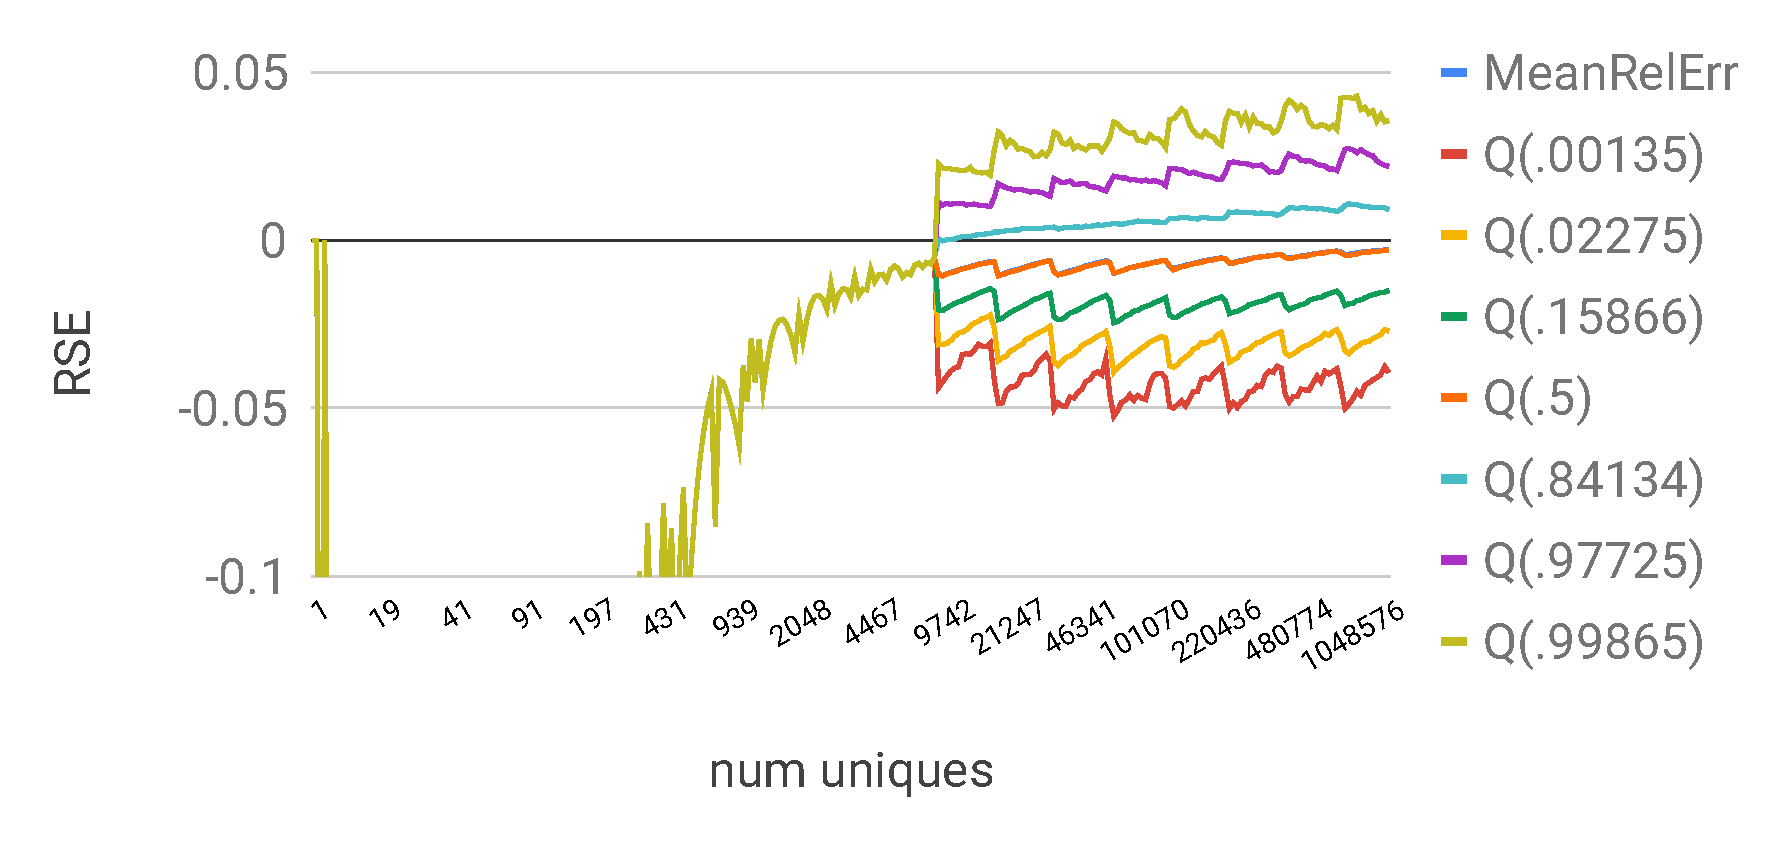
\includegraphics[width=\textwidth]{images/theta-accuracy.pdf}
    \caption{No eager propagation ($e=1.0$)}
    \label{fig:accuracy}
    \end{subfigure}
    \begin{subfigure}{\columnwidth}\centering
    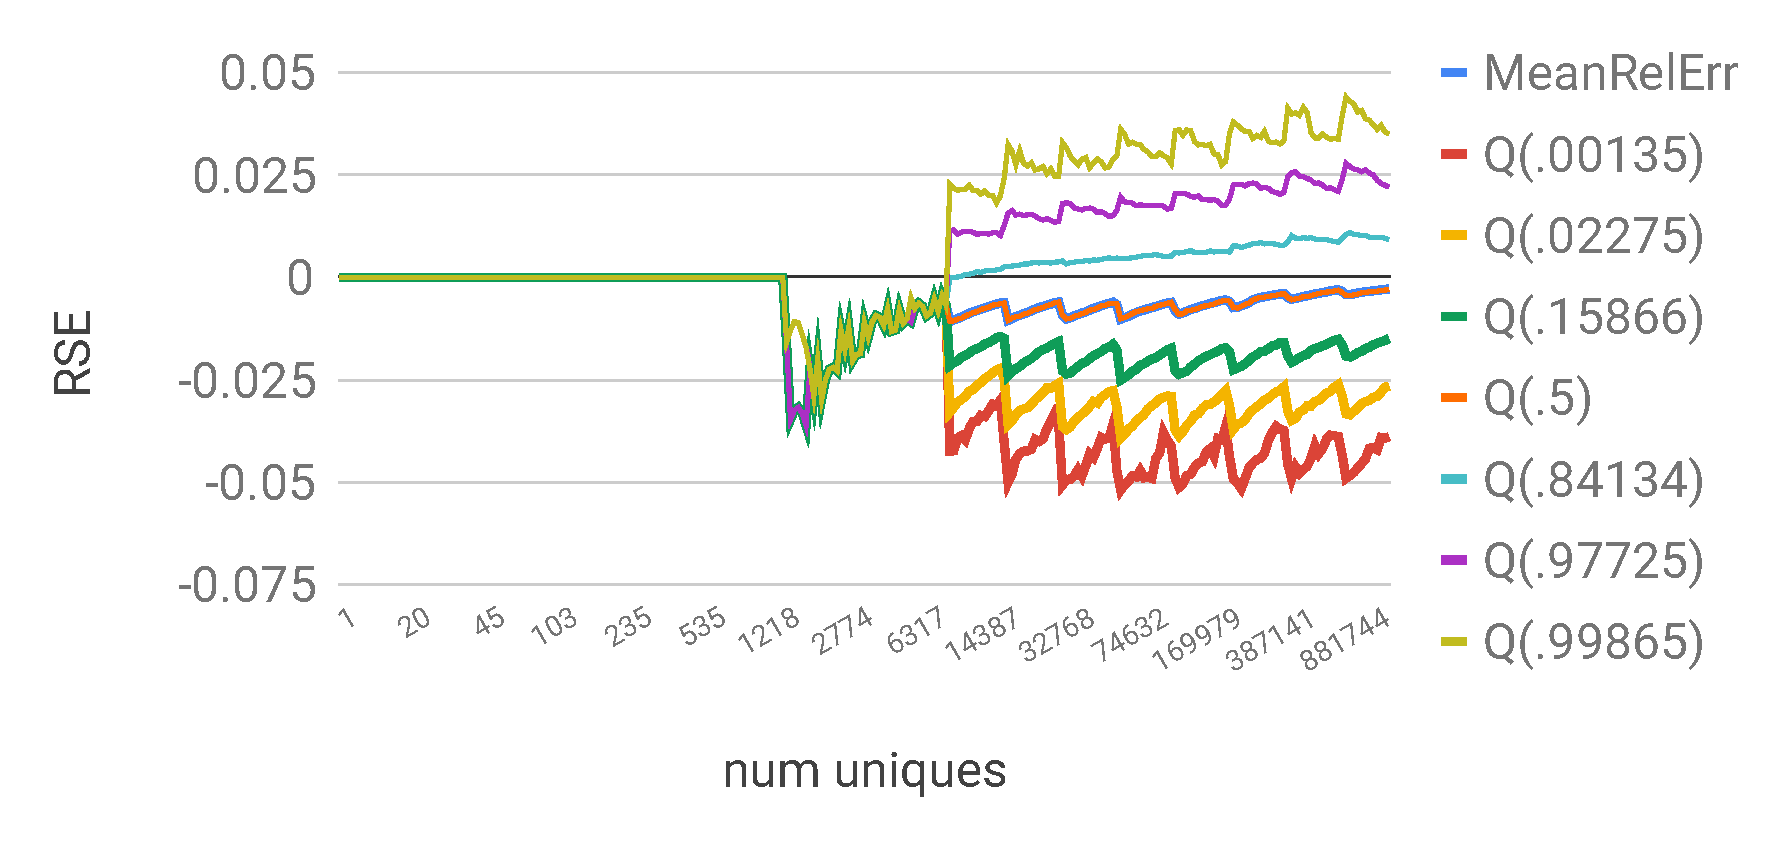
\includegraphics[width=\textwidth]{images/theta-accuracy-adaptive.pdf}
    \caption{With eager propagation, error bound defined by $e=0.04$}
    \label{fig:accuracy-adaptive}
    \end{subfigure}
      \caption{Concurrent $\Theta$ measured quantiles vs RSE, $k = 4096$.}
      \label{fig:accuracy-res}
\end{figure*}

\paragraph{Write-only workload}
Figure~\ref{fig:throughput:native} presents throughput measurements for a write-only workload. The results are shown in loglog scale.
Figure~\ref{fig:throughput:large} zooms-in on the throughput of large streams.

When considering large stream sizes, the concurrent implementation scales with the number of threads, peaking at
almost $300$M operations per second with $12$ threads. The performance of the lock-based implementation, on the other hand,
degrades as the contention on the lock increases. Its peak performance is
$25$M operations per second with a single thread. Namely, with a single thread, the concurrent $\Theta$ sketch outperforms the lock-based implementation
by $12$x, and with $12$ threads by more than $45$x. 

For small streams, wrapping a single thread with a lock is the most efficient method. Once the stream
contains more than $200$K unique values, using a concurrent sketch with $4$ or more local threads is more efficient.
The crossing point where a single local buffer is faster than the lock-based implementation is around $700$K unique values.
 
\begin{figure*}[tb]
\setlength{\abovecaptionskip}{0pt}
\setlength{\belowcaptionskip}{0pt}
\setlength\textfloatsep{0pt}
\centering
\begin{subfigure}{1.3\columnwidth}\centering
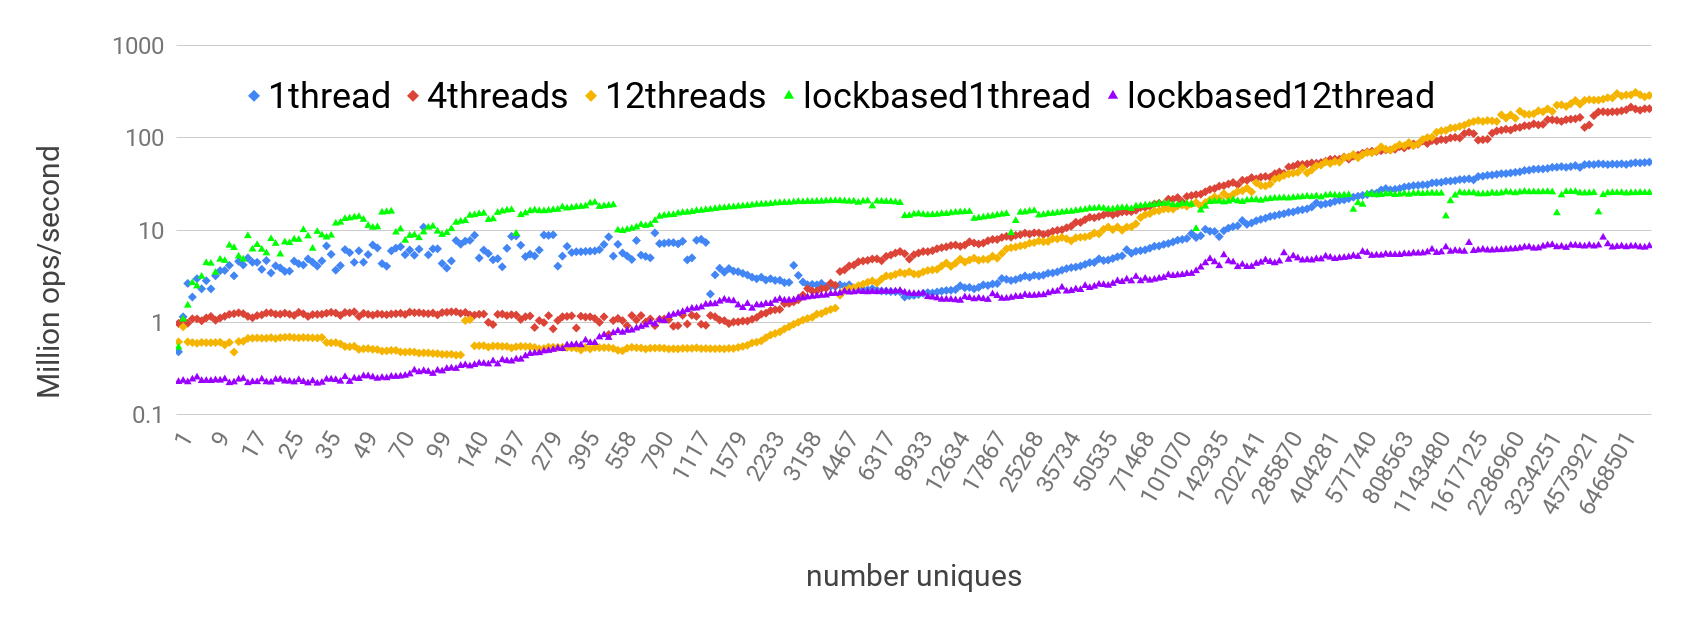
\includegraphics[width=\textwidth]{images/theta-write-only.png}
\caption{Throughput, loglog scale}
\label{fig:throughput:native}
\end{subfigure}
\begin{subfigure}{0.7\columnwidth}\centering
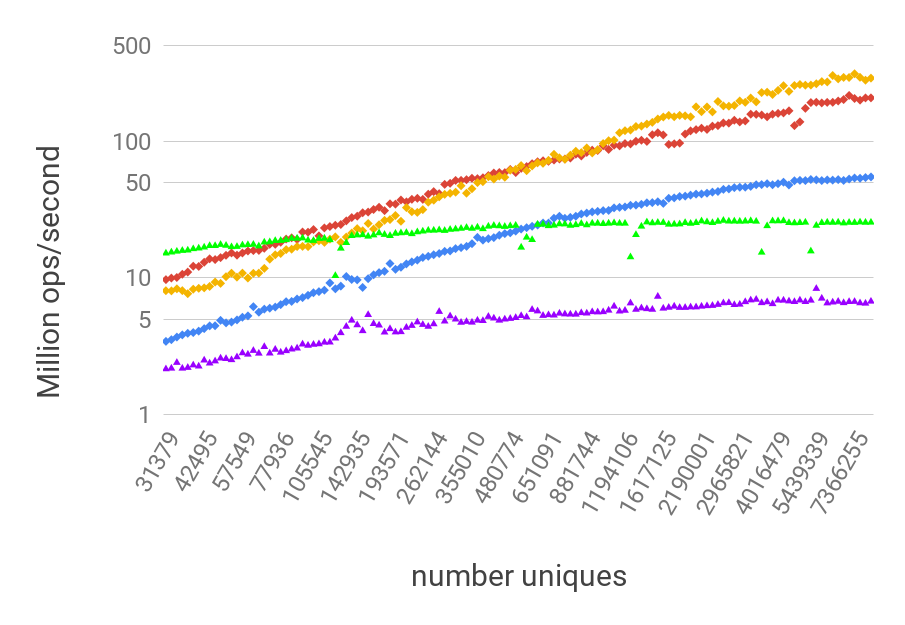
\includegraphics[width=\textwidth]{images/theta-write-only-zoomin.png}
\caption{Zooming-in on large sketches}
\label{fig:throughput:large}
\end{subfigure}
  \caption{Write-only workload, $k = 4096$, $e=0.04$.}
  \label{fig:throughput}
\end{figure*}


\paragraph{Mixed workload}
Figure~\ref{fig:mixed-throughput} presents the throughput measurements
of a mixed read-write workload. We compare runs with a single updating thread and $2$
updating threads (and $10$ background reader threads).
Although we see similar trends as in the write-only workload, the effect of
background readers is more pronounced in the lock-based implementation than in the concurrent one;
this is expected as the reader threads compete for the same lock as the writers.
The peak throughput of a single writer thread in the concurrent implementation is $55$M ops/sec both with and
without background readers. The peak throughput of a single writer thread in the lock-based
implementation degrades from $25$M ops/sec without background reads to $23$M ops/sec with them; this is an almost $10$\% slowdown in performance.
Recall that in this scenario reads are infrequent, and so the degradation is not dramatic.

\begin{figure}[tb]
\setlength{\abovecaptionskip}{0pt}
\setlength{\belowcaptionskip}{0pt}
\setlength\textfloatsep{0pt}
	\centering
	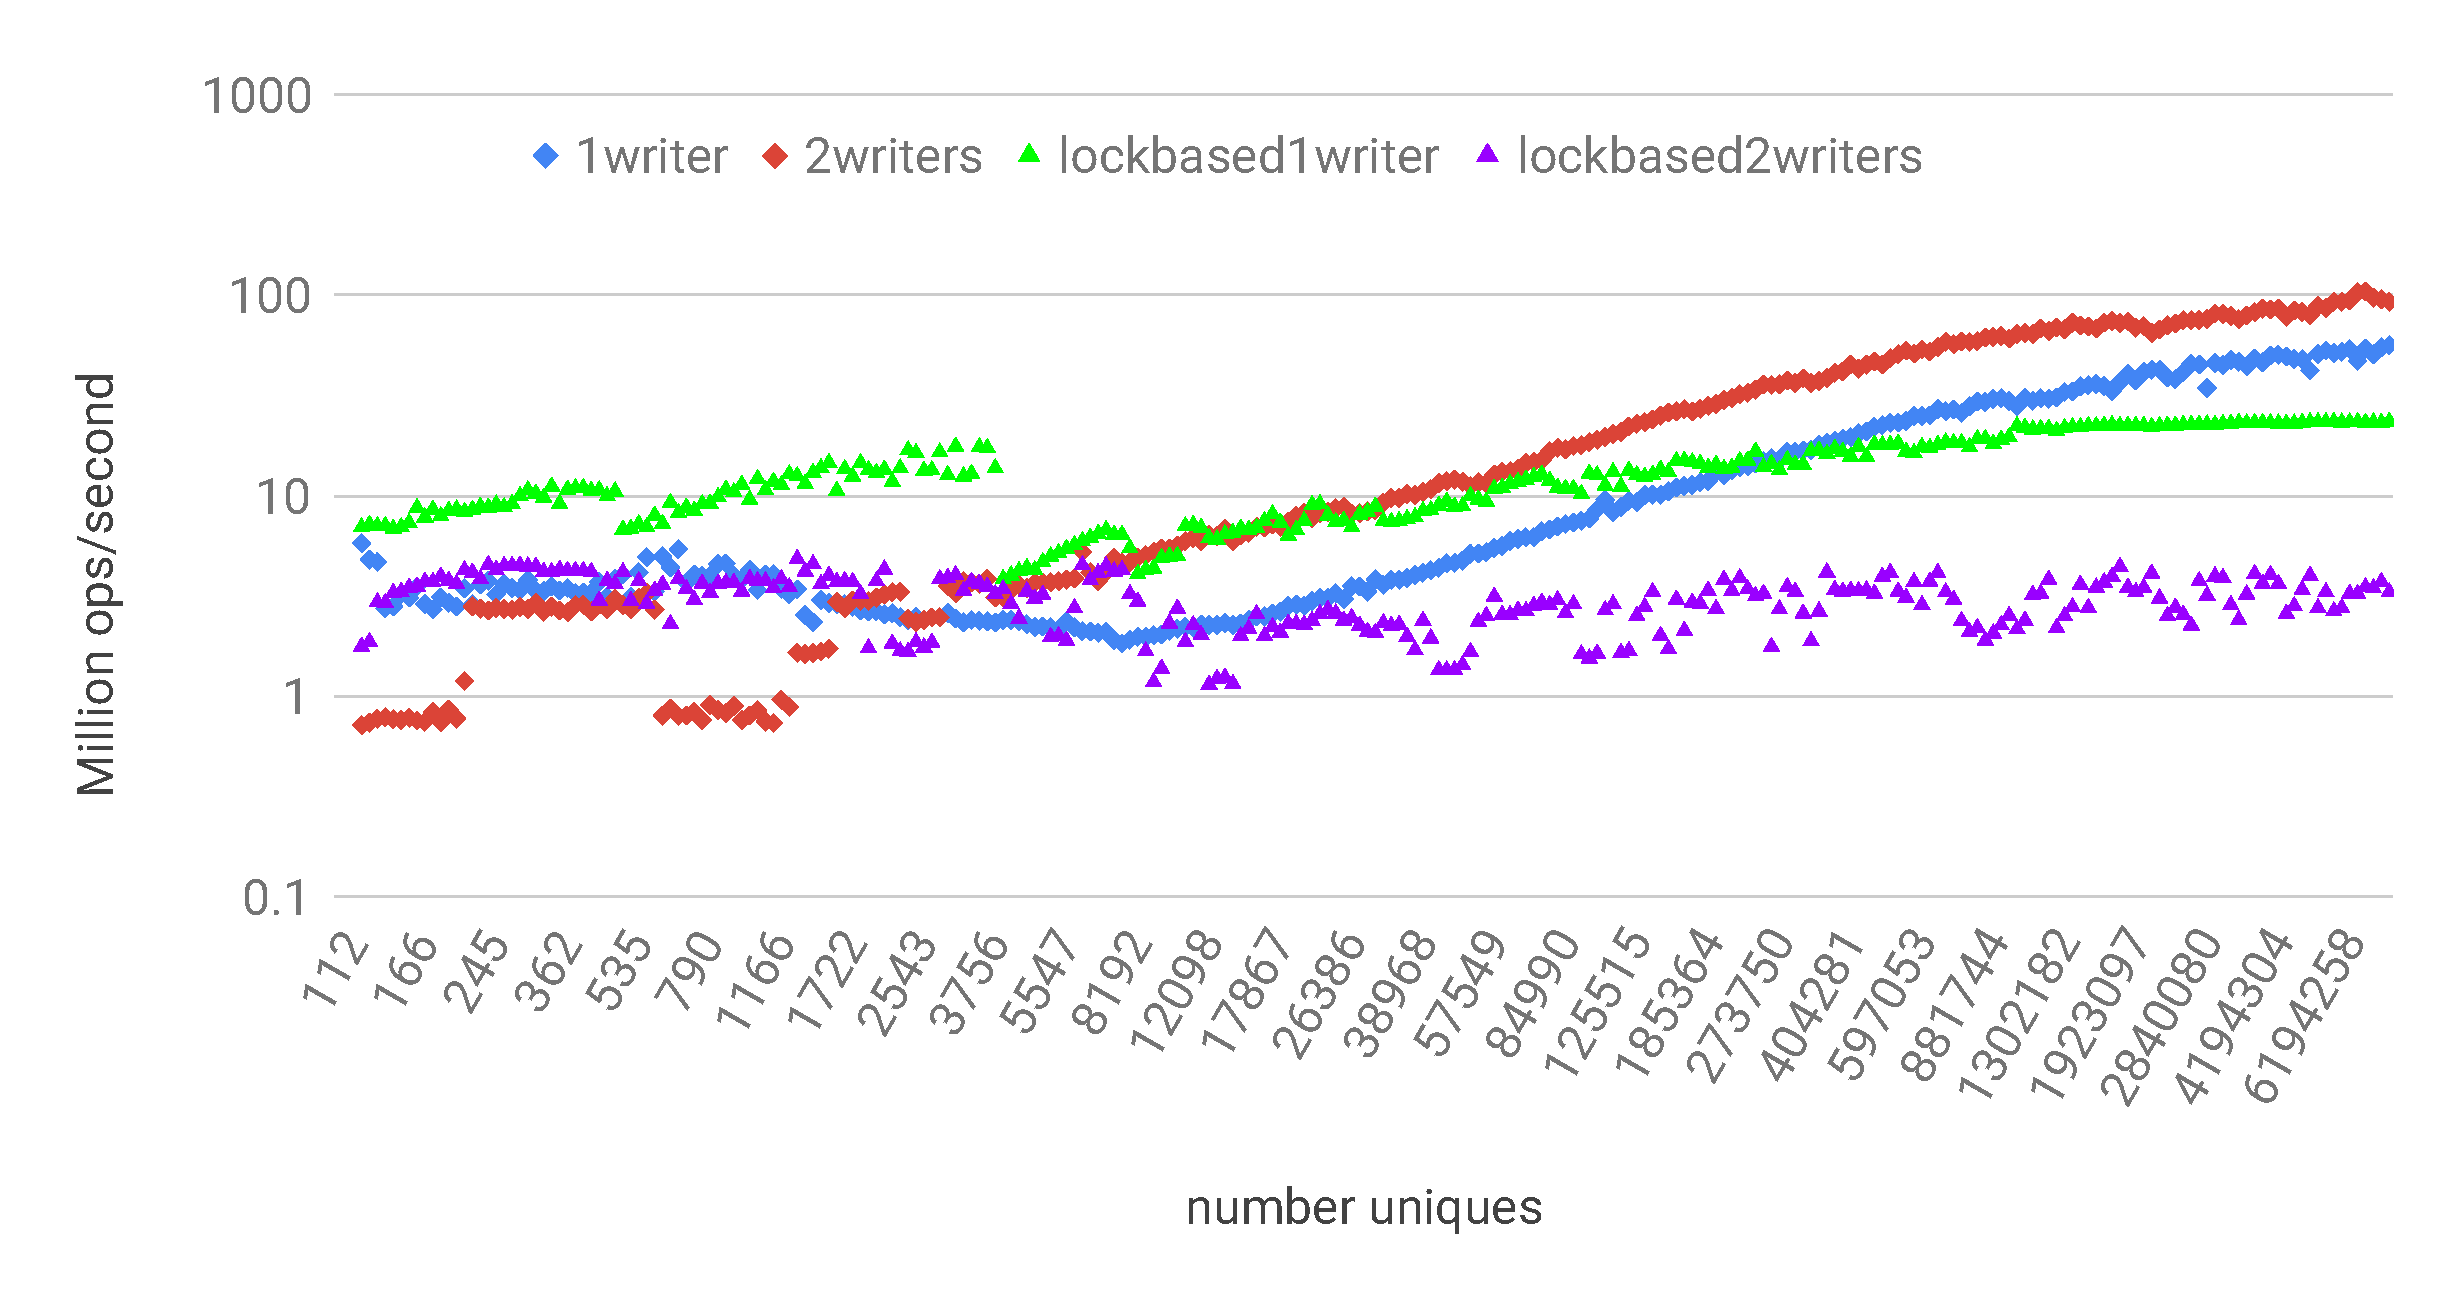
\includegraphics[width=\columnwidth]{images/theta-mixed.pdf}
	\caption{{Mixed workloads: writers with background reads, $k = 4096$, $e=0.04$.}}
	\label{fig:mixed-throughput}
\end{figure}


\paragraph{Scalability results}
To provide a better scalability analysis, we aim to maximize the number of threads working on the
sketch. Therefore, we run this test on a larger machine -- we use a 32-core Xeon E5-4650 processors.
We ran an \emph{update-only} workload in which a sketch is built from a very large stream, repeating
each test 16 times.

In Figure~\ref{fig:performance} (in the introduction) we compare the scalability
of our concurrent $\Theta$ sketch and the original sketch wrapped
with a read/write lock in an update-only workload, for $b=1$ and $k=4096$.
As expected, the lock-based sequential sketch does not scale, and
in fact it performs worse when accessed concurrently by many threads.
In contrast, our sketch achieves almost perfect scalability.
$\Theta$ quickly becomes small enough to allow filtering out most of the updates and so the
local buffers fill up slowly.


\subsection{Accuracy-throughput tradeoff}
\label{ssec:tradeoffs}

The speedup achieved by eager propagation in small streams is presented in Figure~\ref{fig:speedup}.
This is an additional advantage of eager propagation in small streams, beyond the accuracy benefit reported in Figure~\ref{fig:accuracy-res}. 
The improvement is as high as $84$x for tiny sketches, and tapers off as the sketch grows.
The slowdown in performance when the sketch size exceeds $2k$ can be explained by the reduction
in the local buffer size (from $b=16$ to $b=5$), needed in order to accommodate for the required error bound.

\begin{figure}[tb]
\setlength{\abovecaptionskip}{0pt}
\setlength{\belowcaptionskip}{0pt}
\setlength\textfloatsep{0pt}
	\centering
	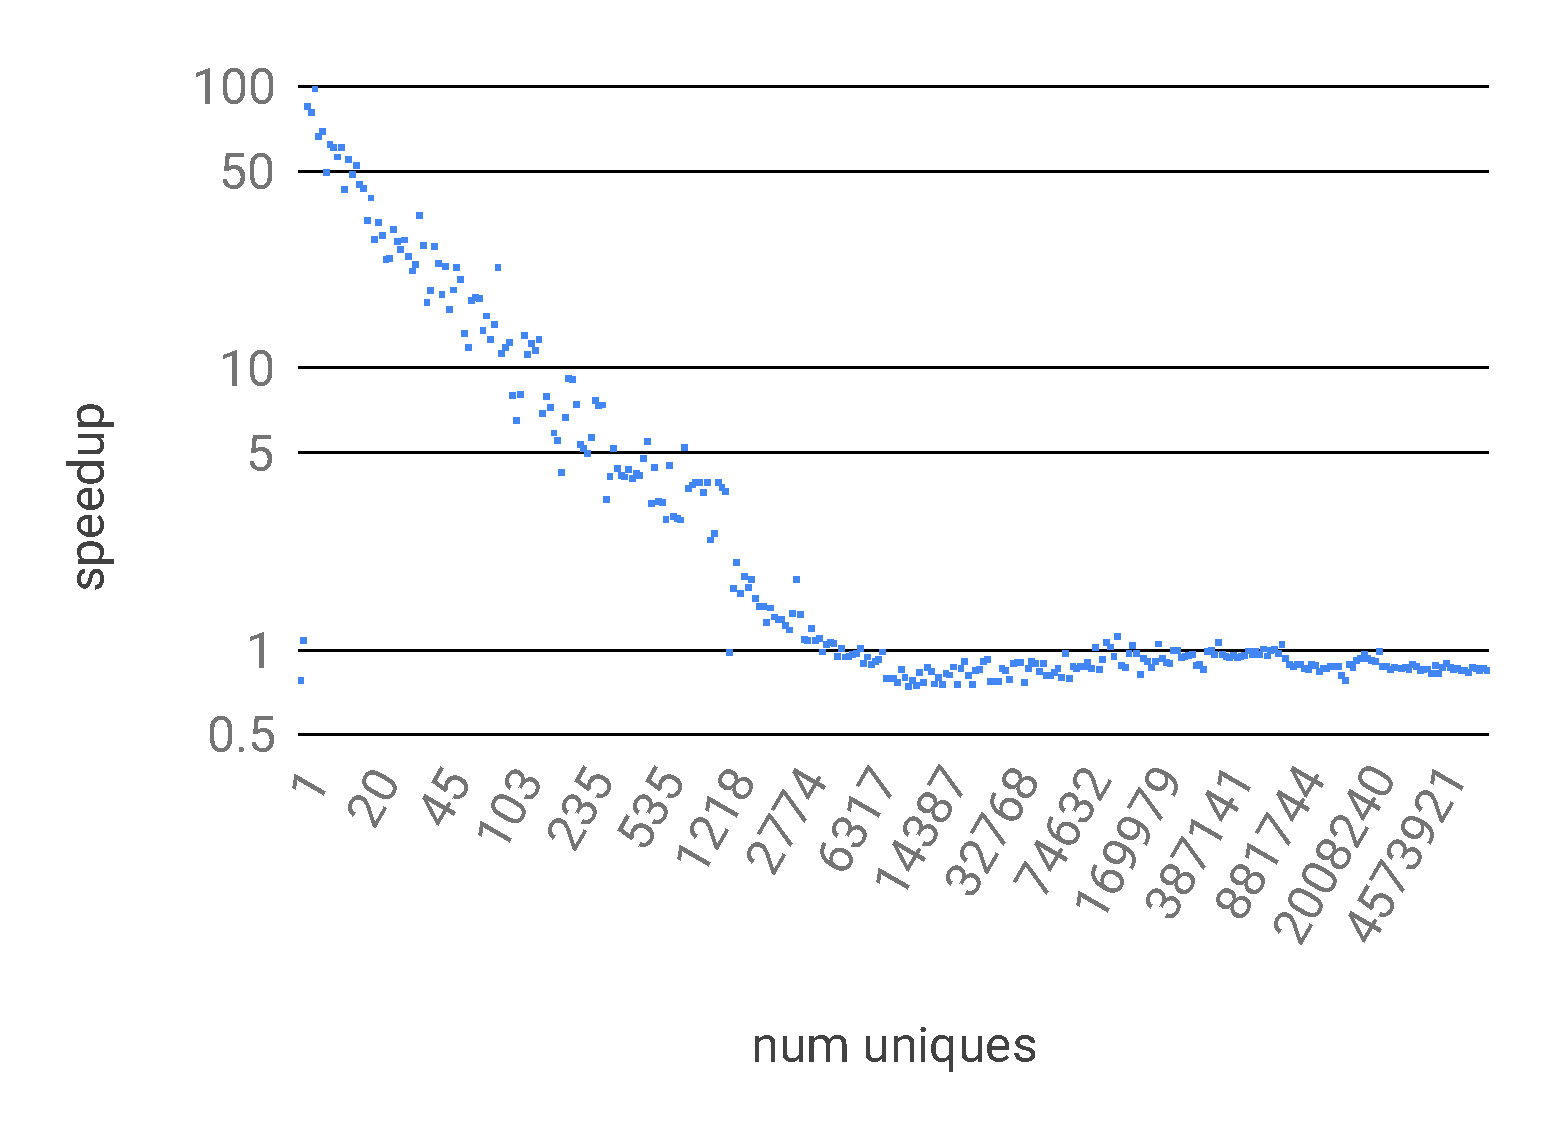
\includegraphics[width=\columnwidth]{images/eager-speedup.pdf}
	\caption{{Throughput speedup of eager ($e=0.04$) vs no-eager ($e=1.0$) propagation, $k = 4096$.}}
	\label{fig:speedup}
\end{figure}


Next we discuss the impact of $k$.
One way to increase the throughput of the concurrent $\Theta$ sketch is by
increasing the size of the global sketch, namely increasing $k$. On the other hand,
this change also increases the error of the estimate.
Table~\ref{tab:tradeoff} presents the tradeoffs between performance and accuracy.
Specifically, it presents the crossing-point, namely the smallest stream size for which the concurrent
implementation outperforms the lock-based implementation (both running a single thread). It further presents
the maximum values (across all stream sizes) of the median error and 99th percentile error for a variety of $k$ values.
The table shows that as the sketch promises a smaller error (by using a larger $k$), a larger stream size is needed to justify using
the concurrent sketch with all its overhead.

\begin{table}[htb]
\center{\small{
\begin{tabular}{lrrr}
\hline 
& thpt crossing point & mean error & error $Q=0.99$ \\
\hline 
$k=256$ &  15,000 &	0.16 & 0.27 \\
\hline 
$k=1024$ &  100,000 &	0.05 & 0.13 \\
\hline 
$k=4096$ & 700,000	& 0.03	& 0.05	\\ 
\hline 
\end{tabular}
}}
\caption{{Performance vs accuracy as a function of $k$.}}
\label{tab:tradeoff}
\end{table}  




%\section{Scalability evaluation}
\label{sec:evaluation}


The purpose of this section is to quantify the scalability of
our  framework. In this context, the adaptation to small streams is irrelevant so we disable it.
%
Our implementation extends the code in Apache DataSketches (Incubating)~\cite{DataSketches}, a Java
open-source library of stochastic streaming algorithms. The $\Theta$ sketch implementation there
differs slightly from the KMV $\Theta$ sketch we  used as a running example, and is
based on a HeapQuickSelectSketch family. In this version, the sketch stores between $k$ and $2k$ items
whilst keeping $\Theta$ as the $k^{th}$ largest value. When the sketch is full,
it is sorted and largest $k$ values are discarded. 

We experimented on a dedicated machine with four Intel
Xeon E5-4650 processors, each with $8$ cores, for a total of
$32$ threads (with hyper-threading disabled).
We ran an \emph{update-only} workload in
which a sketch is built from a very large stream. Repeated experiments showed similar results. 


\begin{figure}[tb]
\setlength{\abovecaptionskip}{0pt}
\setlength{\belowcaptionskip}{0pt}
\setlength\textfloatsep{0pt}
%\begin{wrapfigure}{r}{0.45\textwidth}
  \begin{center}
    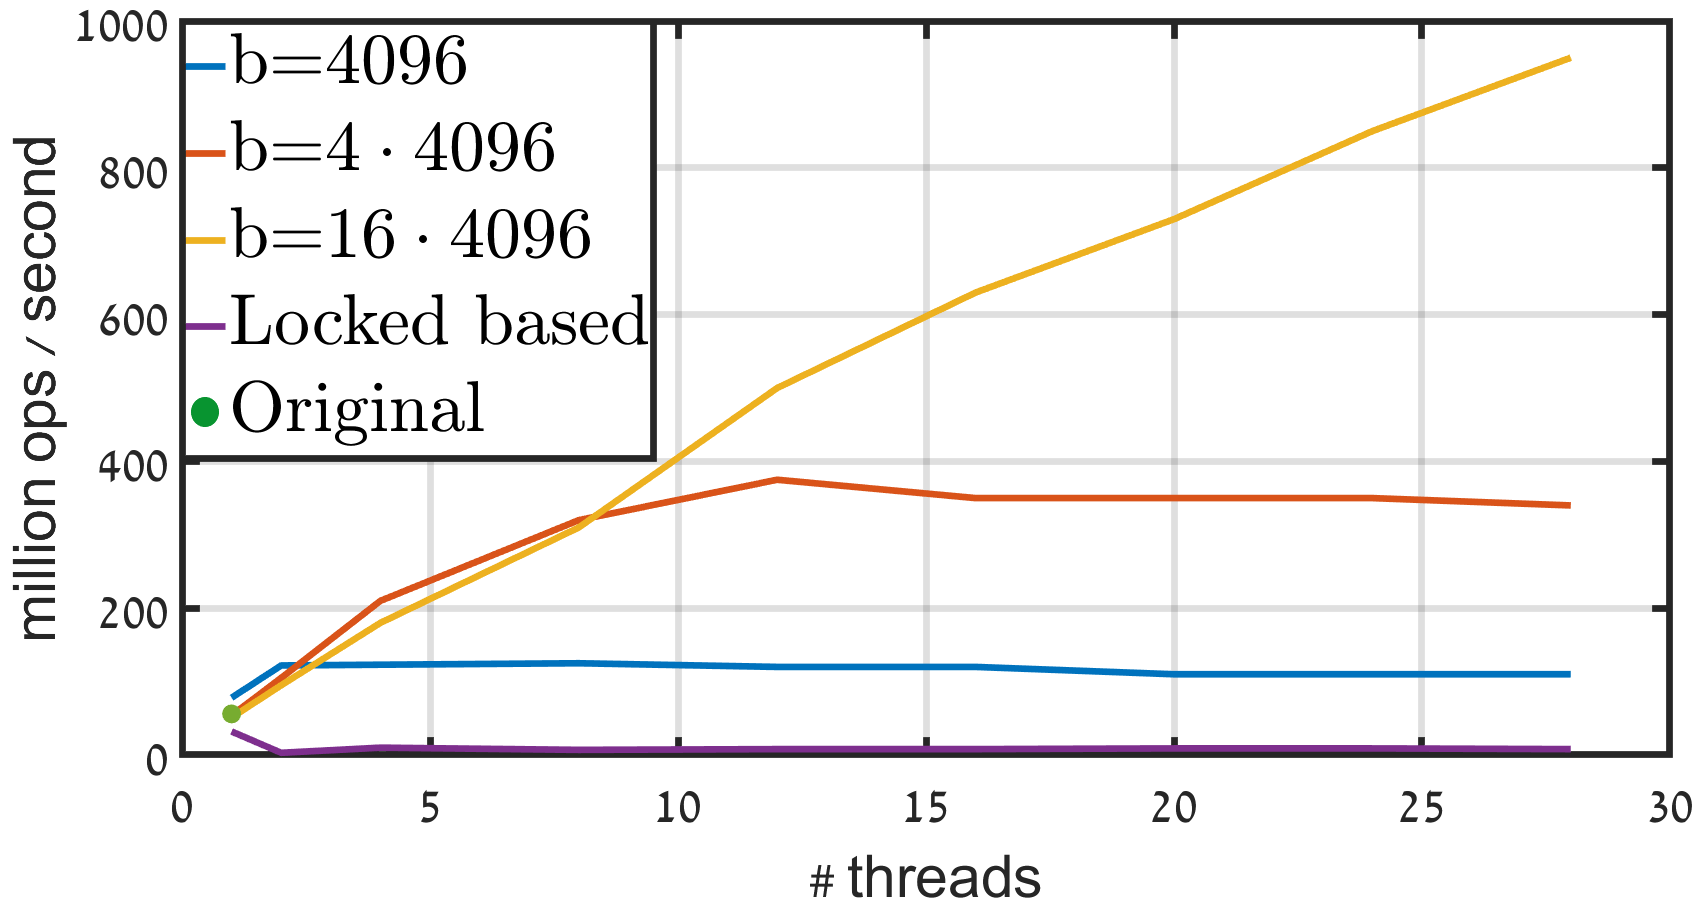
\includegraphics[width=0.44\textwidth]{images/QuantilesUpdate.png}
  \end{center}
  \caption{Scalability of DataSketches' Quantiles sketch 
  protected by a lock vs. our concurrent implementation with different local
  buffer sizes $b$.}
      \label{fig:ConccurentQuantilesUpdate}
%\end{wrapfigure}
\end{figure}





Our baselines are the sequential sketches
from the library, wrapped with a read/write lock
to allow concurrency. Our results show that adding the lock reduces
the single-thread performance of the $\Theta$ sketch
from 90 to 32 million operations per second, and that of the Quantiles
sketch from 77 to 32 million.

In Figure~\ref{fig:performance} (in the introduction) we compare the scalability
of our concurrent $\Theta$ sketch and the original sketch wrapped
with a read/write lock in an update-only workload, for $b=16$ and $k=4096$.
As expected, the lock-based sequential sketch does not scale, and
in fact it performs worse when accessed concurrently by many
threads.
In contrast, our sketch achieves almost perfect scalability.
We also tried smaller local buffers, as small as $b=1$,
and the results were similar; for large streams $\Theta$ sketch
is not sensitive to the buffer size thanks to using shouldAdd to
prune out updates. $\Theta$ quickly
becomes small enough to allow filtering out most of the updates and so even small
local buffers fill up slowly.

Our concurrent Quantiles' snapshot method uses a double collect
on a dedicated \emph{bitmap} variable in the sketch library. This sketch
does not use hints: calcHint returns 1 and shouldAdd always returns true.

In Figure~\ref{fig:ConccurentQuantilesUpdate} we compare the
throughput of our Quantiles sketch to the baseline.
We see that again the baseline achieves the best result with a single worker thread.
Our sketch, in contrast, scales perfectly when every thread
has a sufficiently large local buffer.
But here, in order for the
background thread to support more worker threads, we have to
enlarge the local buffers. This is because, unlike $\Theta$,
we do not use a hint to reduce the frequency of updates to local buffers.
%\section{Evaluating Impact of Stream Size on $\Theta$ Sketch}
\label{sec:eval}
We continue with the $\Theta$ sketch experimentation to demonstrate the impact of the stream size on accuracy and performance. 
%We compare the concurrent theta sketch to a sequential Theta sketch wrapped with a reader-writer lock. 
In these experiments the hardware is a 12-core Intel Xeon E5-2620 machine.
Experiment set-up is described in Section~\ref{ssec:setup}. We then discuss accuracy and performance results. Finally, Section~\ref{ssec:tradeoffs} presents tradeoffs between accuracy and performance, which demonstrate the benefits of our stream size-adaptive algorithm.

\subsection{Setup}
\label{ssec:setup}
\paragraph{Implementation}
Concurrent $\Theta$ sketch is implemented in Java as part of the Apache DataSketches (incubating) project, and is generally available since V0.13.0. 
%We compare it to the sequential Theta sketch wrapped with a reader-writer lock.
The sequential implementation and the sketch at the core of the global sketch in the concurrent implementation are the same (HeapQuickSelectSketch, which is the default sketch family).

Global sketch defines \emph{exact limit} -- the limit between exact mode (eager propagation) and estimate mode (lazy propagation). The limit is a function of a configurable error parameter $e$; the function used in the library is $2/e^2$. 
%
Local sketch defines $b$ to be a function of $k$, $e$ and the maximum number of local threads $N$. $b$ has positive correlation with $e$ and inverse correlation with $N$.

Eager propagation, as described in the pseudo-code, requires context switch which incurs high overhead. In the implementation, either the local thread itself eagerly executes every update to the global sketch (buffer size is 1) or lazily delegates updates to a background propagation thread (buffer size is $b$). The decision is based on the global sketch mode (exact or estimate), which is cached in the local sketch as part of the piggyback process that also updates local theta. 
As long as the global sketch is in exact mode the propagation critical section is protected by a shared boolean flag indicating whether (eager) propagation is in progress. When the global sketch switches to estimate mode it is guaranteed that no eager propagation gets through; instead local threads attempting to update the global sketch via eager propagation get an indication to pass the buffer via lazy propagation.
This implementation ensures (a) local threads avoid costly context switch when the sketch is small, (b) lazy propagation by a background thread is done without synchronization.

Unless otherwise stated sketches are configured with $k = 4096$, and $e=0.04$; Thus the exact limit is $2/e^2=1250$, and $b$ is set (by the implementation) to a value between 1 and 5 to accommodate the error bound.


\paragraph{Workload}
We focus on two simple workloads: (1) write-only  - updating a sketch with a stream of unique ids; (2) mixed read-write workload - updating
a sketch with background readers querying the number of unique ids in the stream. Background reads refer to threads that occasionally
(with 1 ms pauses) query the sketch. This simulates real world scenario where updates are constantly streaming from a feed or multiple
feeds, while queries arrive at lower rate.

In both write-only and read-write workloads we measure only the throughput. We vary the number of threads used to feed
the sketch between 1 to 12. In all read-write benchmarks we exercise 10 background reader threads.
\remove{
We refrain from measuring latency of read operations first, since it is challenging (capturing the duration of a few nanoseconds operation).
Second, while it is clear that reading the state of a Theta sketch without a lock is more efficient than doing so after acquiring a lock,
the effect on the entire end-to-end read operation which may include network latencies is negligible. Therefore, we focus on the effect of locks on ingestion throughput.
}
\paragraph{Framework}
To run the experiments we employ a multi-thread extension of the characterization framework. This is the Apache DataSketch evaluation benchmark suite, which measures both the speed and accuracy of the sketch. 

For measuring write throughput the sketch is fed with a continuous data stream. The size of the stream varies from 1 to 8M uniques. For each size $x$ we measure the time $t$ it takes to feed the sketch $x$ unique values, and present it in term of throughput ($x/t$). To avoid measurements noise, each point on the graph represents an average of many trials. The number of trials is very high ($2^{18}$) for points at the low end of the graph. It gradually decreases as the size of the sketch increases. At the high end (at 8M uniques per trial) the number of trials is 16. 

Accuracy of concurrent $\Theta$ sketch is measured only in a single-thread environment. As in the performance evaluations the $x$-axis represents the number of uniques fed into a sketch by a single writing thread. For each size $x$ one trial logs the estimation result after feeding x unique values to the sketch. In addition, it logs the Relative Error (RE) of the estimate, where RE = MeasuredValue/TrueValue -1. This trial is repeated multiple times (specifically 4K times), logging all estimation and RE results. The $y$-axis are the lines of the mean and some constant quantiles of the distributions of error measured at each $x$-axis point on the graph, including the median. 
This type of graph is called ``pitchfork''. 
\remove{
Example of accuracy plots for the sequential $\Theta$ sketch can be found in~\cite{accuracy-plots}.
}

\subsection{Results}
\label{ssec:res}

\paragraph{Accuracy Results}
The accuracy result of a concurrent $\Theta$ sketch that does not employ eager propagation are presented in Figure~\ref{fig:accuracy}. There are two interesting phenomena to observe. First, it is interesting to see empirical evaluation reflecting the theoretical analysis presented in Section~\ref{ssec:theta-analysis}, and thus the ``pitchfork'' is distorted toward lower estimation. More specifically, mean relative error is smaller than $0$ and values of relative error in all measured quantiles tend to be smaller than the relative error of a sequential implementation (estimating less than a sequential implementation). Thereby increasing or decreasing the absolute error depending on whether the error is negative or positive.

Second, for small streams, when the number of unique items is lower than $2k$, $\theta=1$ and the estimation is simply the number of items propagated to the global sketch. If eager propagation is not applied, the number of items in the global sketch depends on the delay in propagation. The smaller the sketch is the more significant the delay is, and the mean error reaches as high as 94\% (we capped the error in the figure at 10\%). As the size of the sketch becomes closer to $2k$ the delay in propagation (of last 16 updates) is less significant, and the mean error decreases.
Obviously, most analytic systems today cannot tolerate such high error. For this the algorithm applies eager propagation until the global sketch reaches the desired exact limit. 
Figure~\ref{fig:accuracy-adaptive} depicts the accuracy results when applying eager propagation. Indeed, the error at small streams (smaller than 8k unique items) is less than 4\%.
%This guided us in introducing the adaptive flavour of the algorithm (discussed in Section~\ref{sec:small-streams}) whose performance results are presented in the next section.

\begin{figure*}[tb]
\setlength{\abovecaptionskip}{0pt}
\setlength{\belowcaptionskip}{0pt}
\setlength\textfloatsep{0pt}
\centering
\begin{subfigure}{\columnwidth}\centering
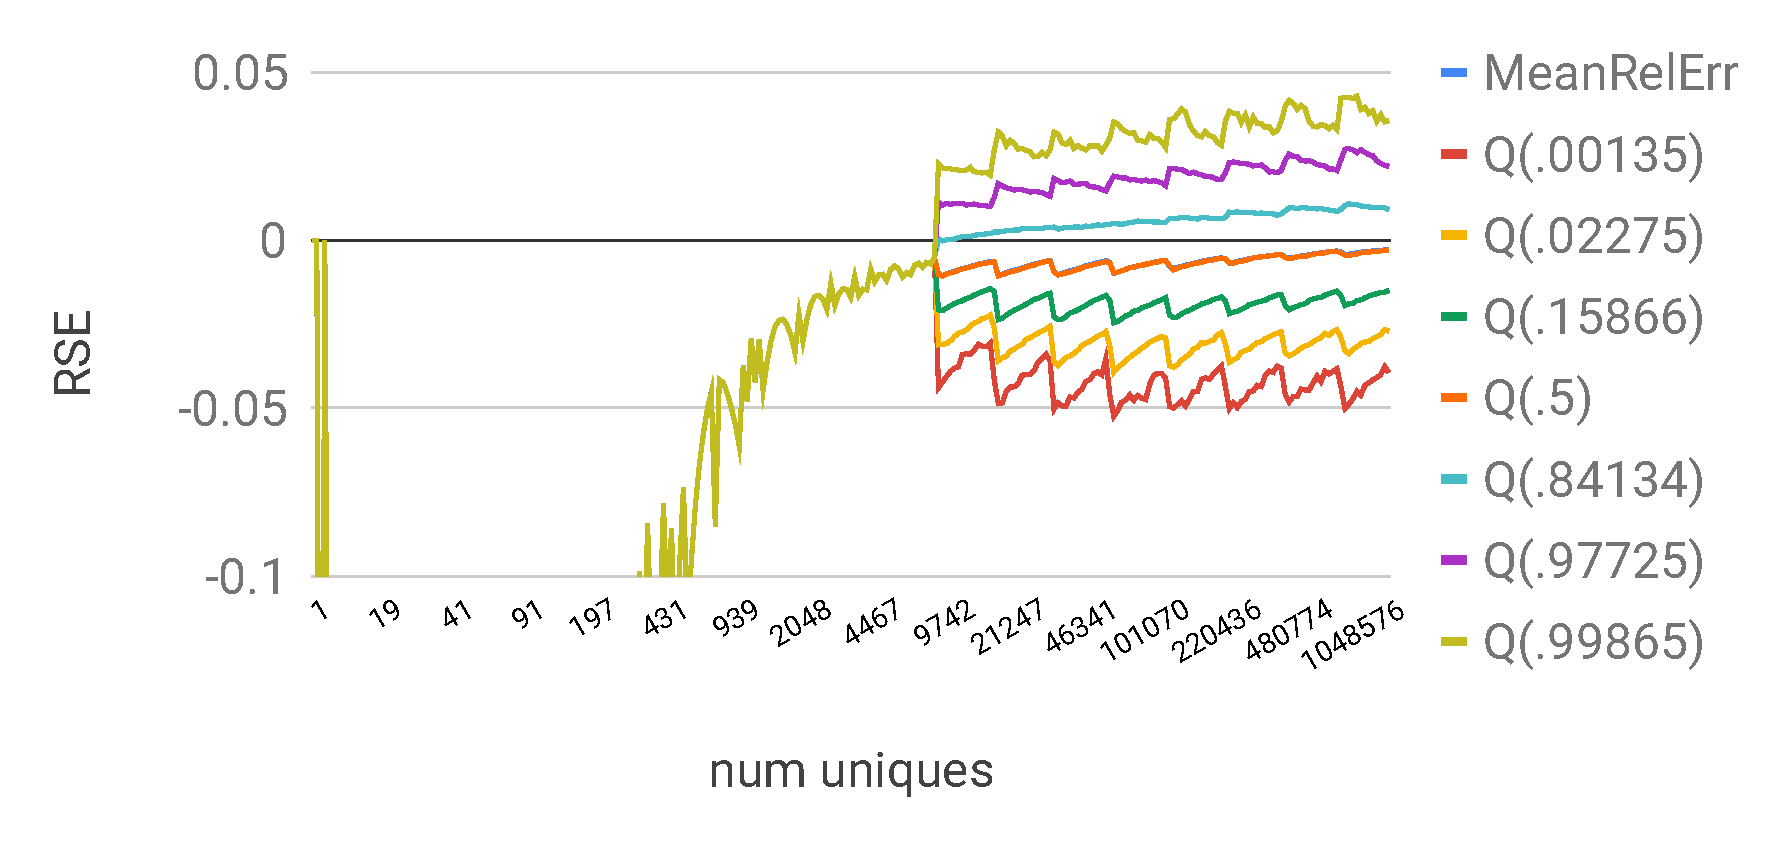
\includegraphics[width=\textwidth]{images/theta-accuracy.pdf}
\caption{No eager propagation ($e=1.0$)}
\label{fig:accuracy}
\end{subfigure}
\begin{subfigure}{\columnwidth}\centering
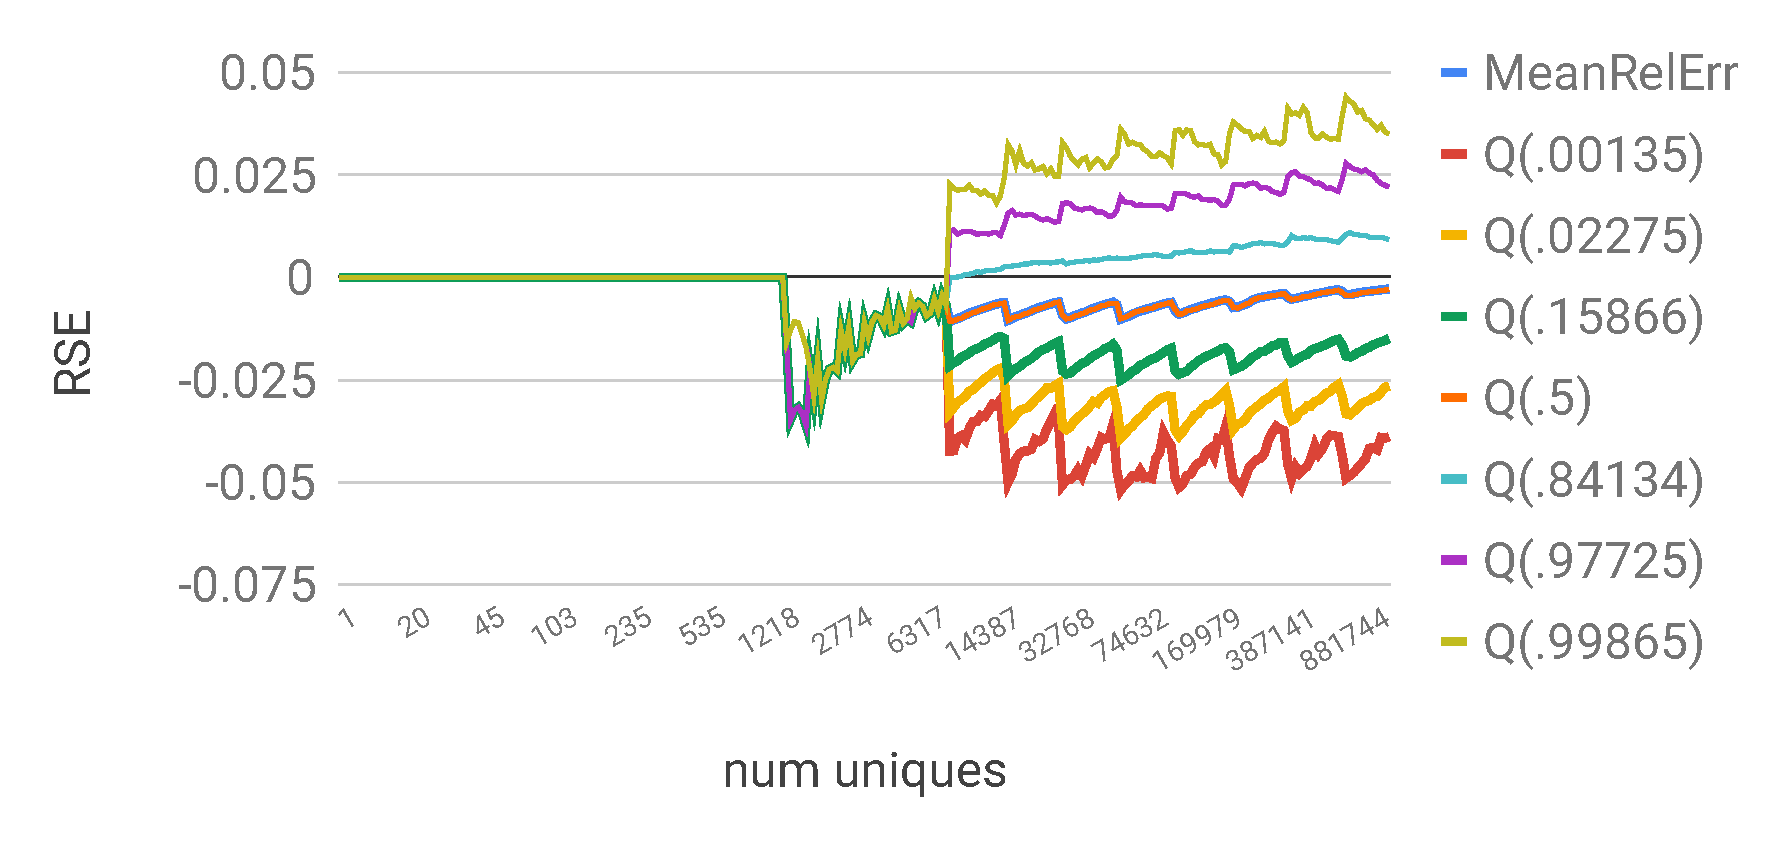
\includegraphics[width=\textwidth]{images/theta-accuracy-adaptive.pdf}
\caption{With eager propagation, limit defined by $e=0.04$}
\label{fig:accuracy-adaptive}
\end{subfigure}
  \caption{Concurrent Theta Measured Quantiles vs RSE, $k = 4096$.}
  \label{fig:accuracy-res}
\end{figure*}

\paragraph{Write-only Throughput}
Figure~\ref{fig:throughput:native} presents throughput measurements of write-only workload. The results are shown in loglog scale.
%It compares concurrent theta implementation vs. lock-based theta implementation. 
Figure~\ref{fig:throughput:large} zooms-in on the throughput of large sketches.

When considering large sketches, the concurrent implementation scales with the number of threads; peaking at almost 300M ops/sec with 12 threads. The performance of lock-based implementation, on the other hand, degrades as the contention on the lock increases with the number of threads. Its peak performance is at 25M ops/sec with a single thread. Namely, the concurrent $\Theta$ sketch outperforms lock-based implementation by 12x, and when comparing the performance of 12 threads, concurrent implementation outperforms lock-based implementation by more than 45x. 

For small streams, wrapping a single thread with a lock is the most efficient method. When the stream contains more than 200K unique values, using concurrent sketch with 4 or more local threads is more efficient. The crossing point of a single local buffer over lock-based implementation is arround 700K uniques.
 
\begin{figure*}[tb]
\setlength{\abovecaptionskip}{0pt}
\setlength{\belowcaptionskip}{0pt}
\setlength\textfloatsep{0pt}
\centering
\begin{subfigure}{1.3\columnwidth}\centering
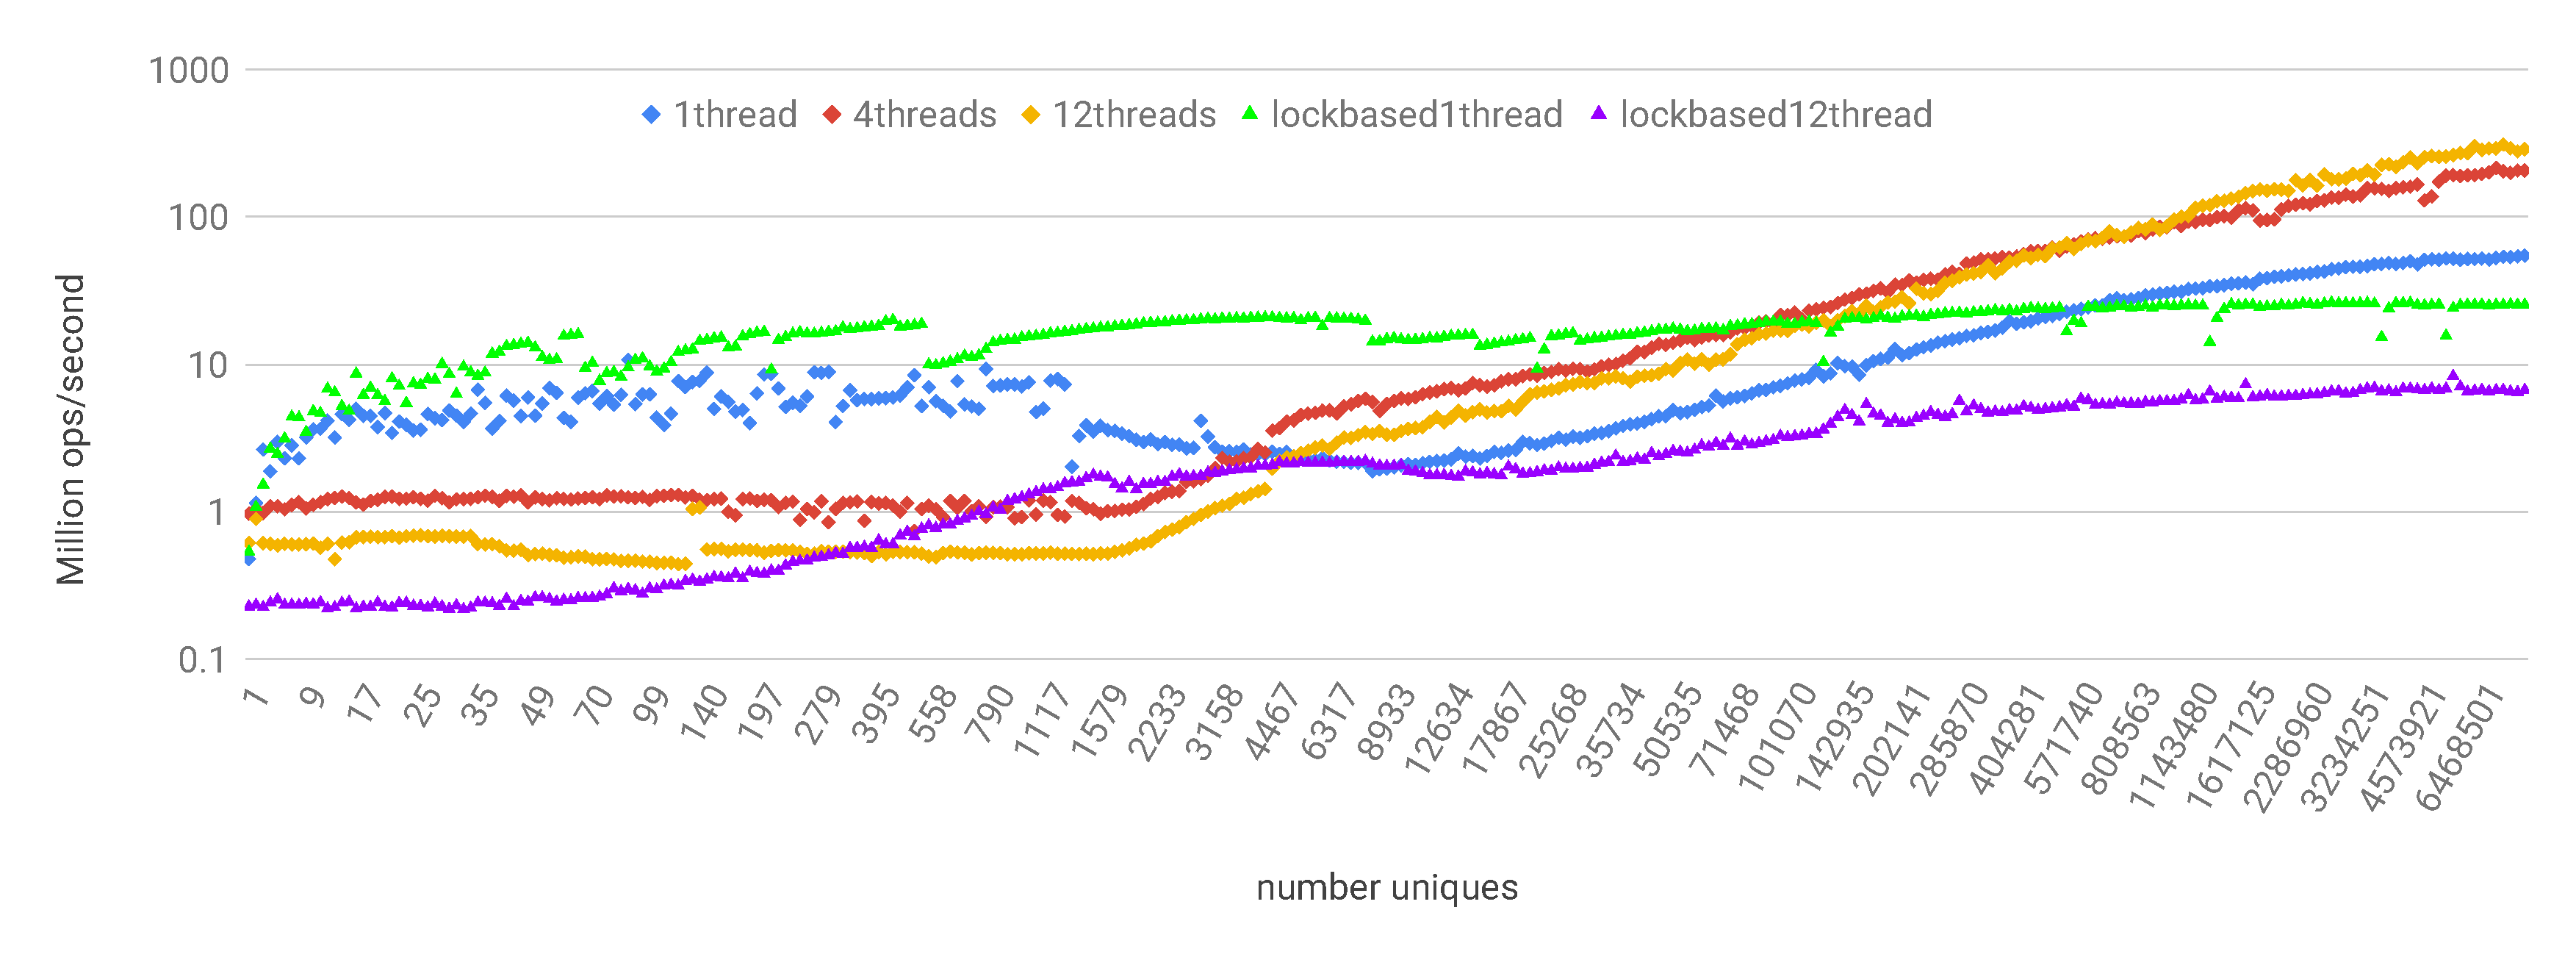
\includegraphics[width=\textwidth]{images/theta-write-only.pdf}
\caption{Throughput, loglog scale}
\label{fig:throughput:native}
\end{subfigure}
\begin{subfigure}{0.7\columnwidth}\centering
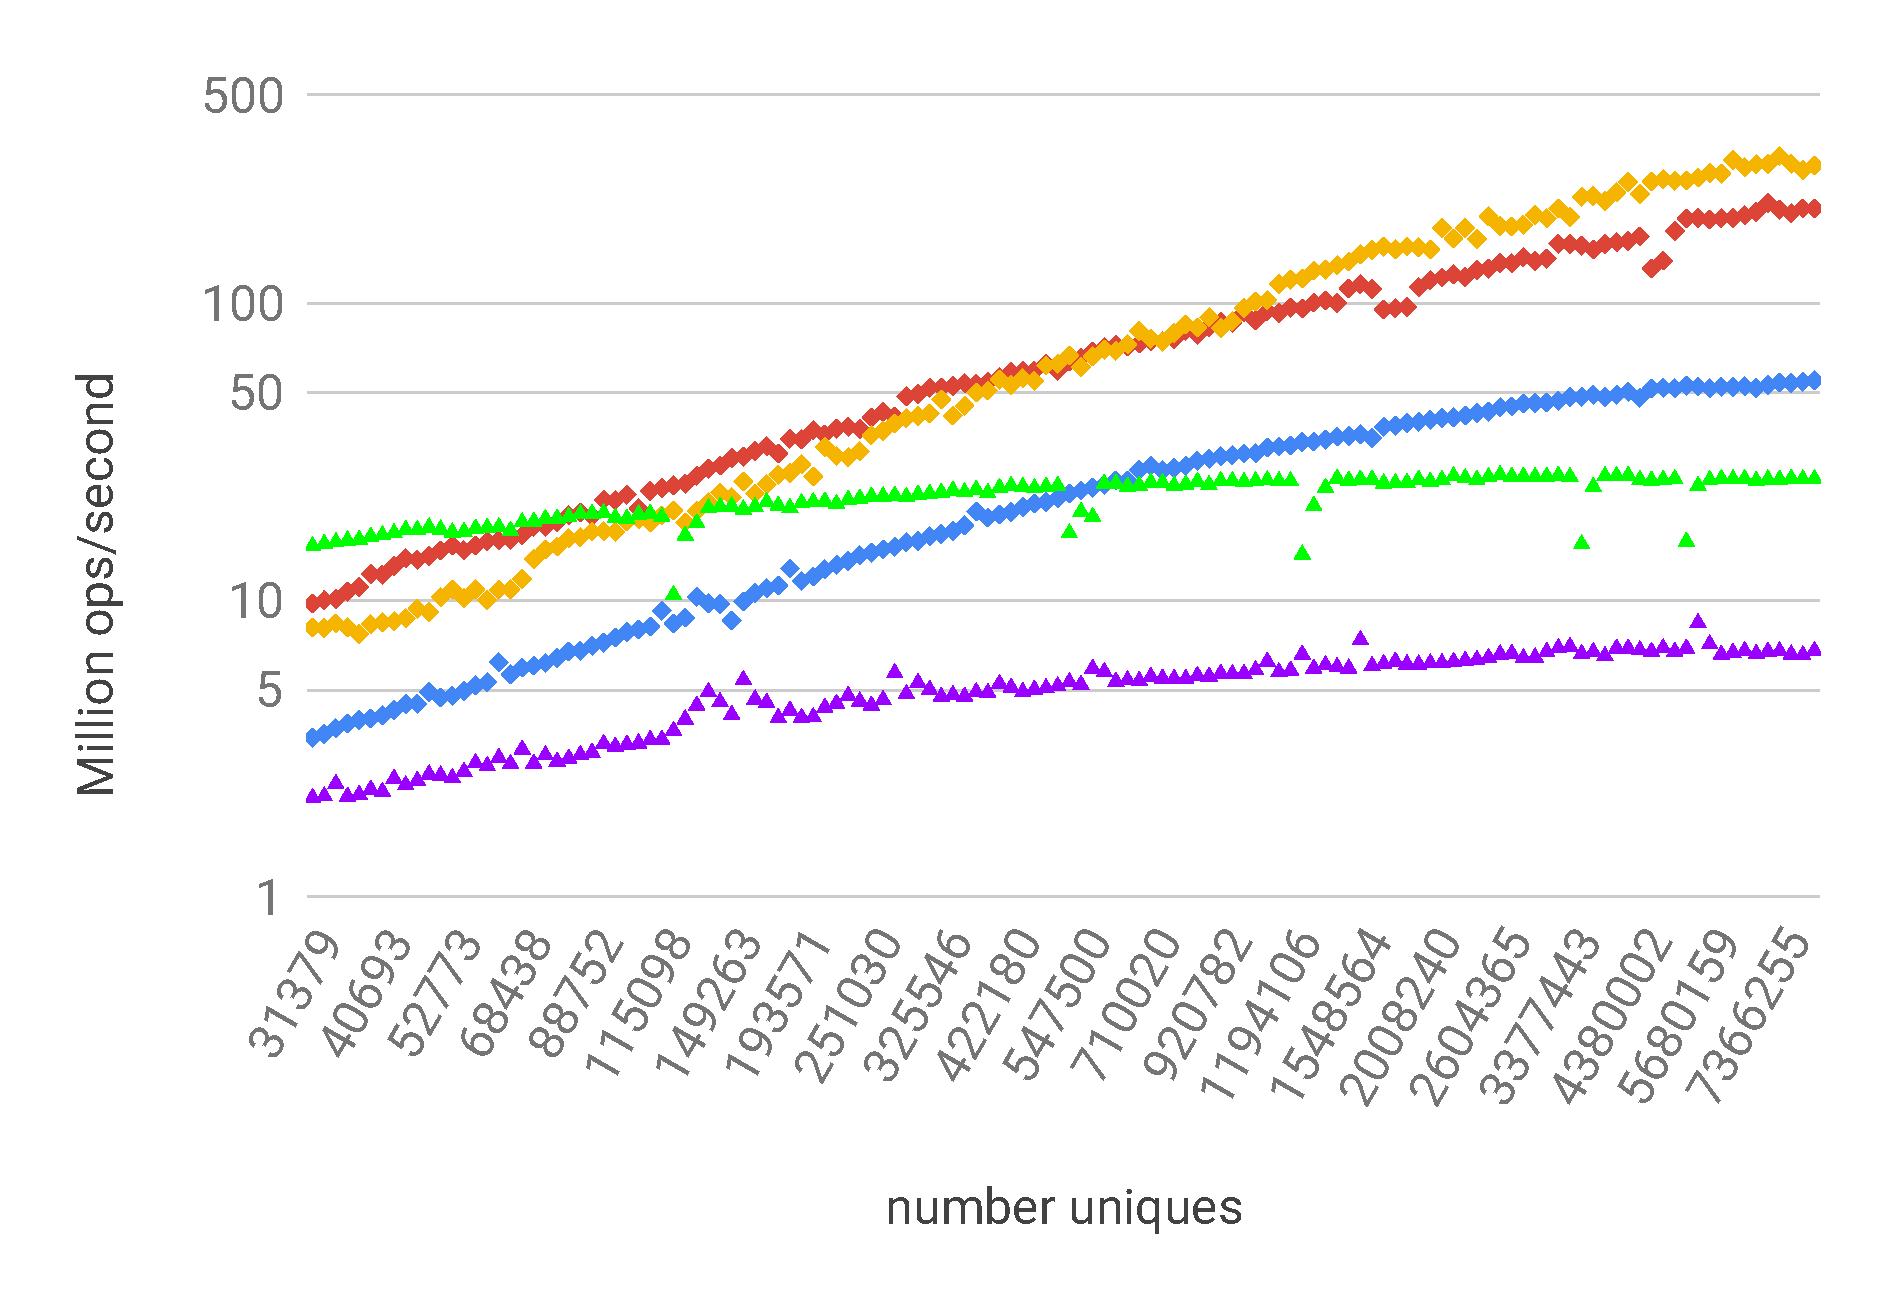
\includegraphics[width=\textwidth]{images/theta-write-only-zoomin.pdf}
\caption{Zooming-in on large sketches}
\label{fig:throughput:large}
\end{subfigure}
  \caption{Write-only workload, $k = 4096$, $e=0.04$.}
  \label{fig:throughput}
\end{figure*}

\paragraph{Mixed Workload}
Figure~\ref{fig:mixed-throughput} presents throughput measurements of mixed read-write workload. We compare runs with a single updating thread and 2 updating threads (and 10 background reader threads).
Here we see similar trends as in the write-only workload. However, the effect of  background readers is more pronounced in lock-based implementation than in concurrent $\Theta$ sketch. The peak throughput of a single writer-thread in the concurrent implementation is 55M ops/sec with and without background readers. The peak throughput of a single writer thread in the lock-based implementation degrades from 25M to 23M ops/sec; almost $10$\% slowdown in performance. And recall that this is when readers are not very frequent.

\begin{figure}[tb]
\setlength{\abovecaptionskip}{0pt}
\setlength{\belowcaptionskip}{0pt}
\setlength\textfloatsep{0pt}
	\centering
	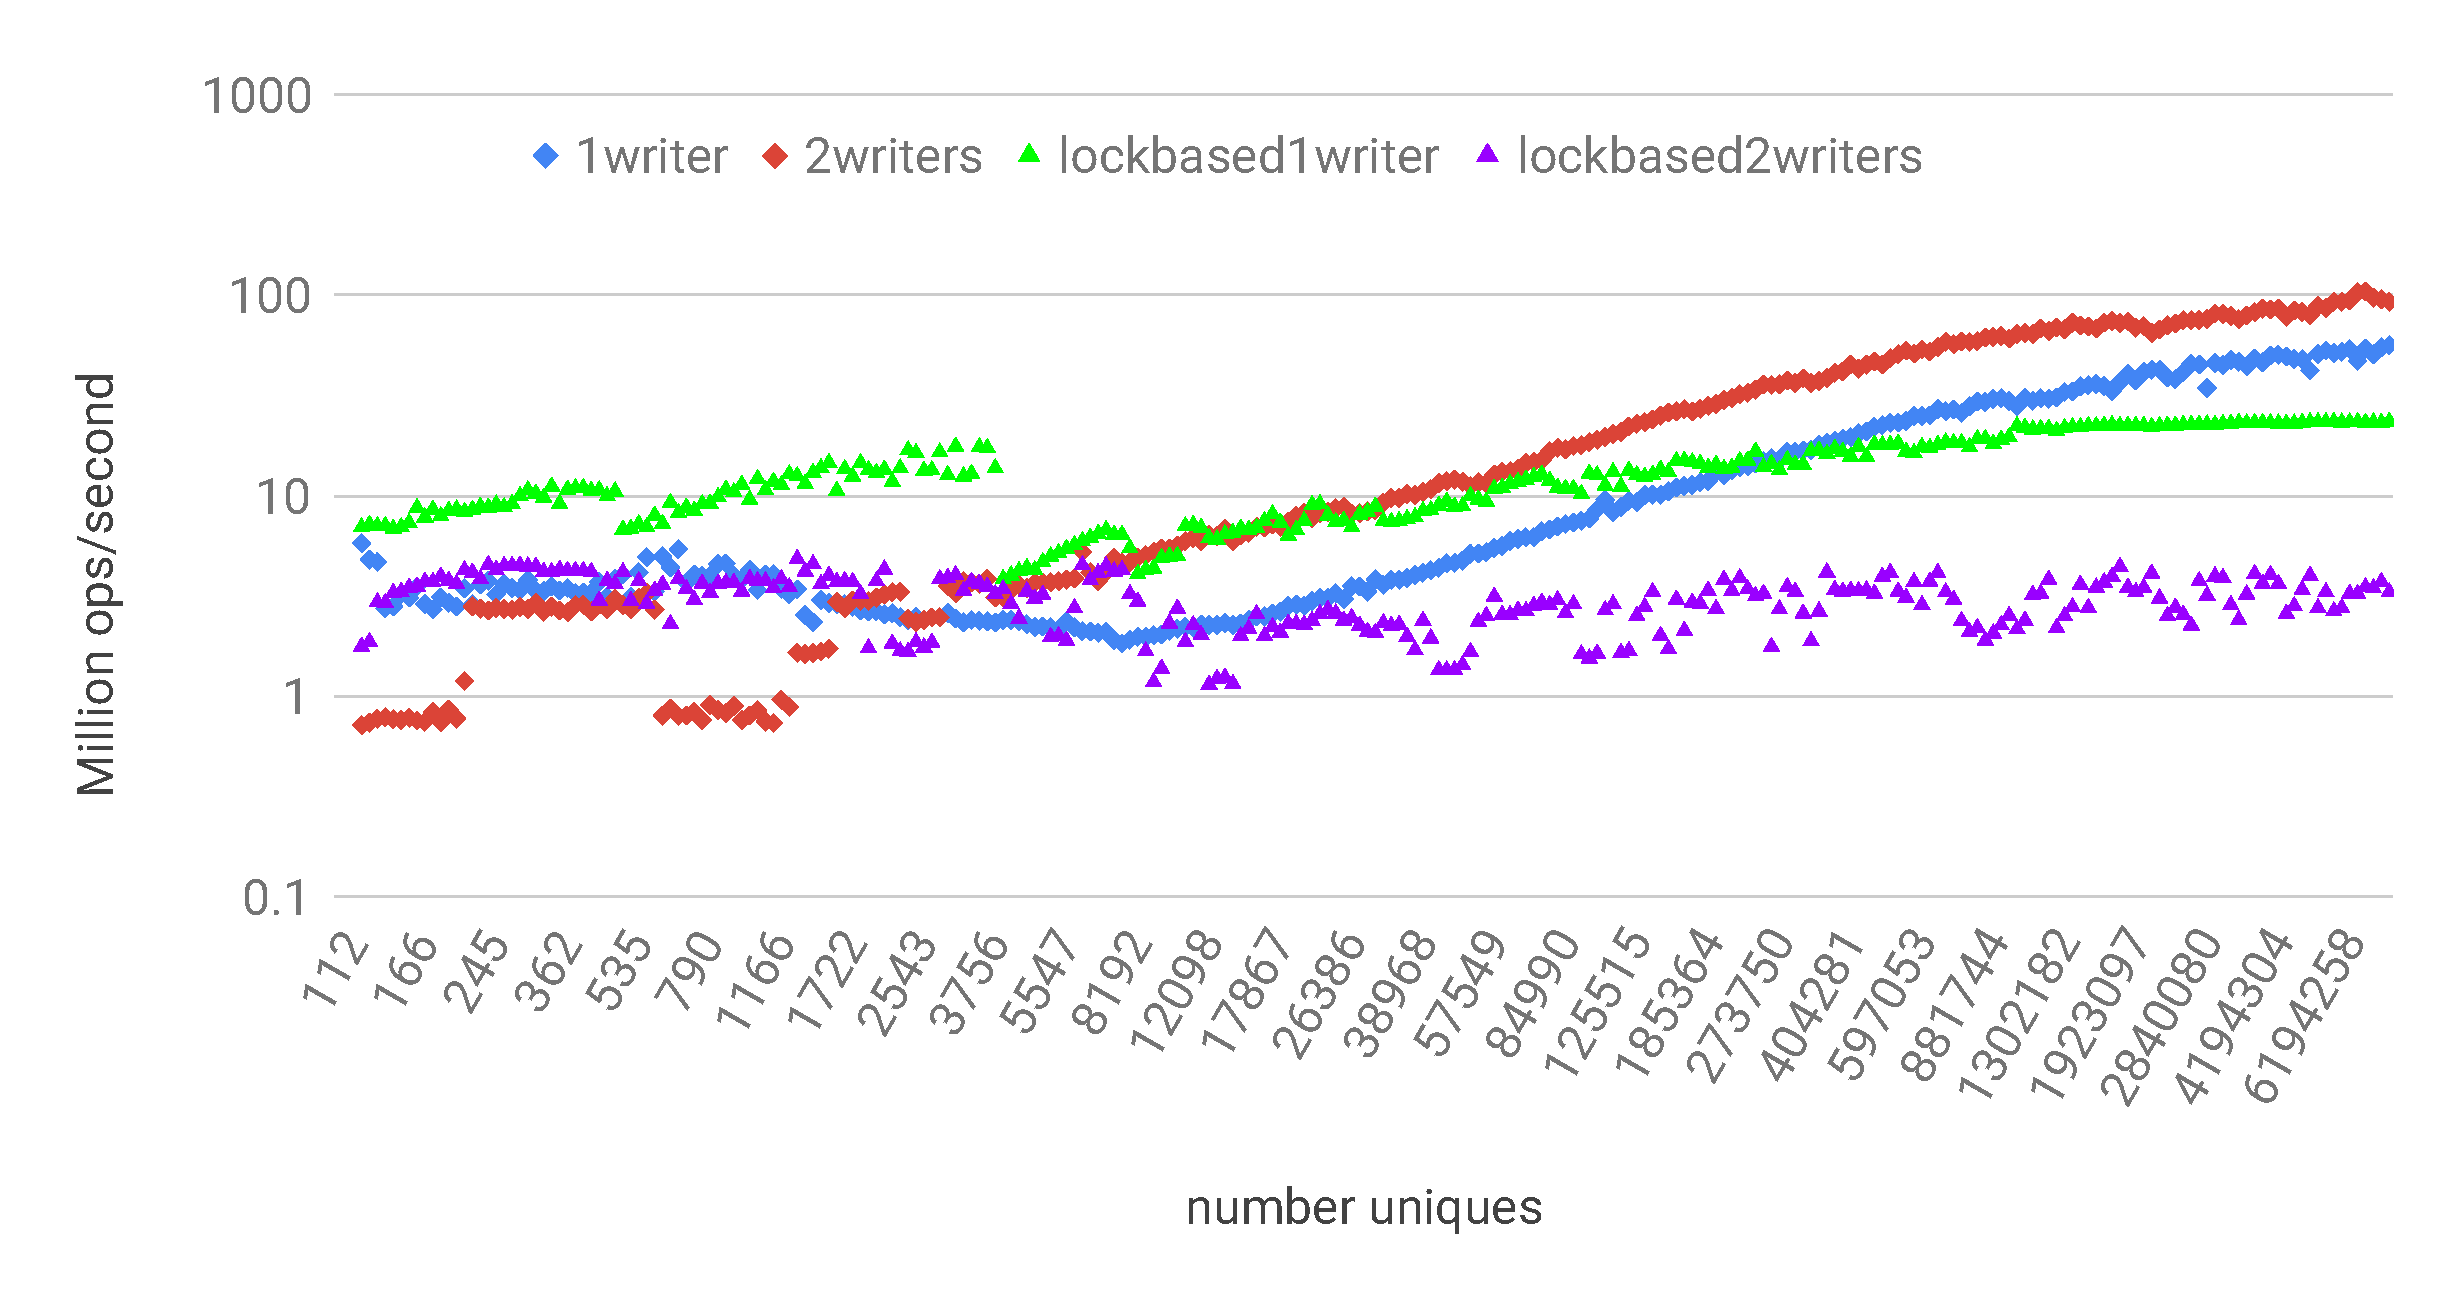
\includegraphics[width=\columnwidth]{images/theta-mixed.pdf}
	\caption{{Mixed workloads: writers with background reads, $k = 4096$, $e=0.04$.}}
	\label{fig:mixed-throughput}
\end{figure}


\subsection{Accuracy-Throughput Tradeoffs}
\label{ssec:tradeoffs}

Eager vs no-eager speedup is presented in Figure~\ref{fig:speedup}. It demonstrates the speedup of eager propagation over no-eager propagation for small streams, in addition to the accuracy benefit reported in Figure~\ref{fig:accuracy-res}. 
The improvement goes up to 84x throughput for tiny sketches, and decreases as the sketch grows. %since the improvement potential is smaller.
The slowdown in performance when the sketch size exceed $2k$ can be explained by the reduction in local buffer size (from $b=16$ to $b=5$) in order to accommodate for the required error bound.

\begin{figure}[tb]
\setlength{\abovecaptionskip}{0pt}
\setlength{\belowcaptionskip}{0pt}
\setlength\textfloatsep{0pt}
	\centering
	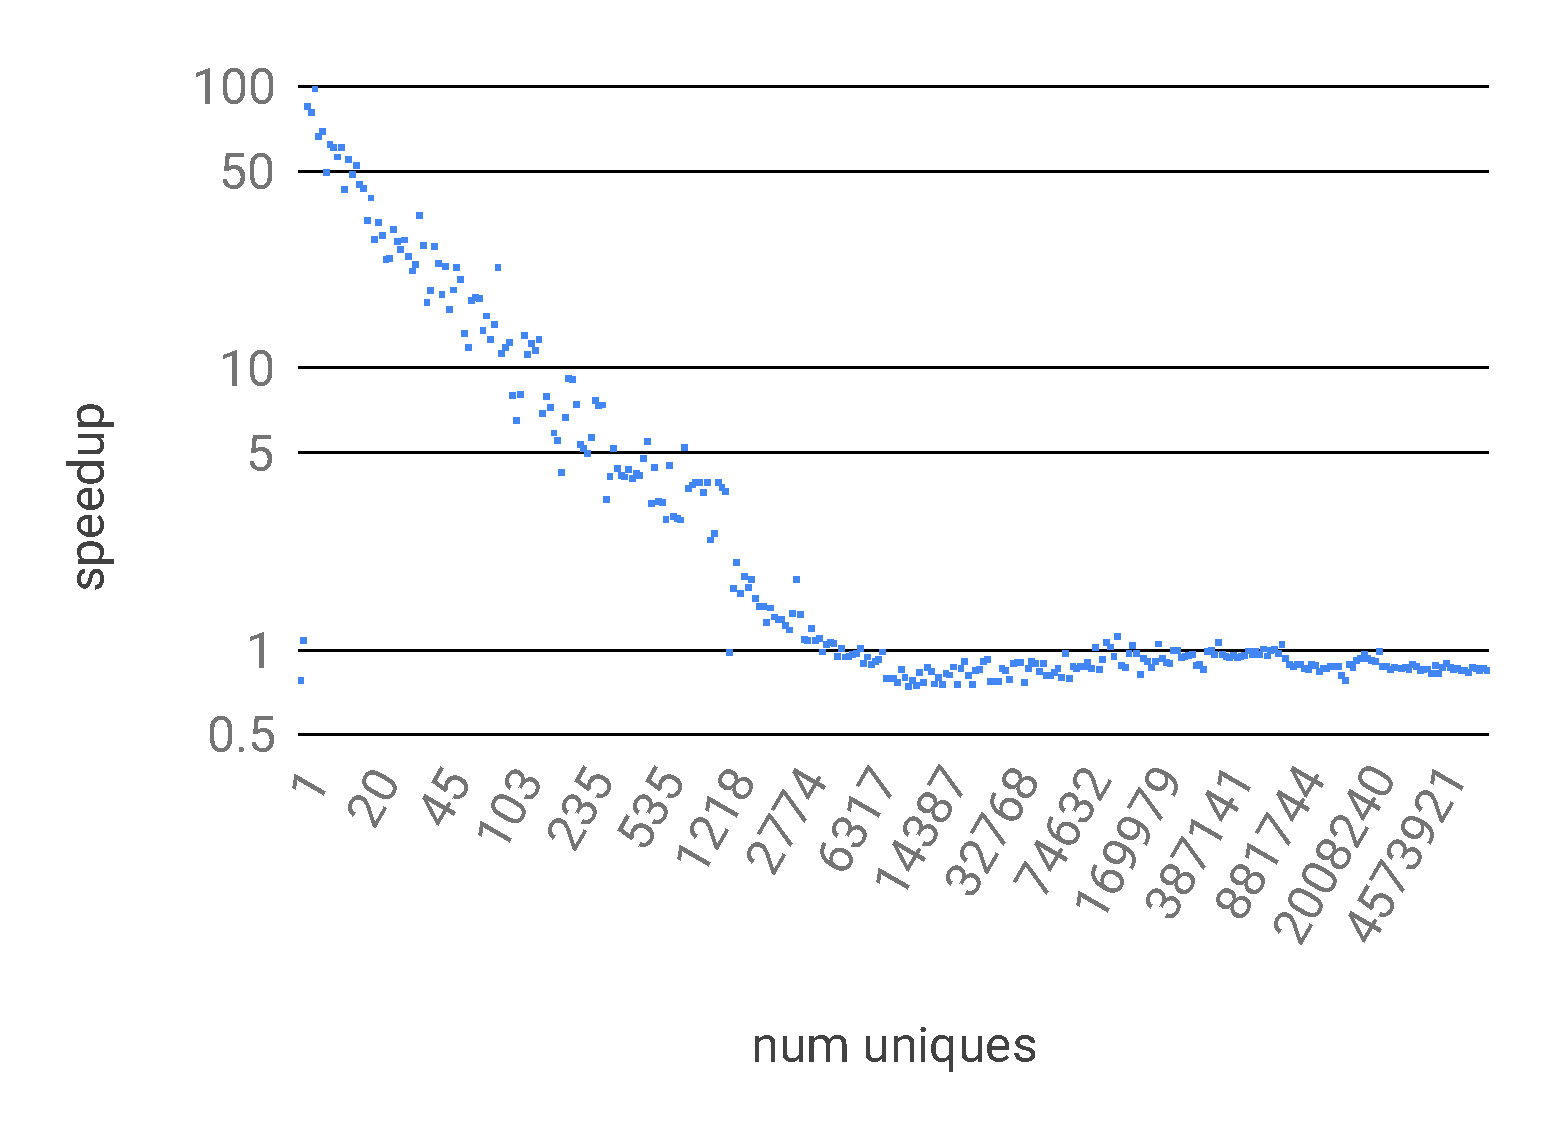
\includegraphics[width=\columnwidth]{images/eager-speedup.pdf}
	\caption{{Throughput speedup of eager ($e=0.04$) vs no-eager ($e=1.0$) propagation, $k = 4096$.}}
	\label{fig:speedup}
\end{figure}


Next we discuss the impact of $k$.
One way to increase the throughput of the concurrent $\Theta$ sketch is by increasing the size of the global sketch, namely increasing $k$. On the other hand, this change also increases the error of the estimate.
Table~\ref{tab:tradeoff} presents the tradeoffs between performance and accuracy. Specifically, it presents the crossing-point, the size of the sketch where concurrent implementation outperforms lock-based implementation (both running a single thread), the maximum values (across sketch sizes) of the median error, and 99th percentile error for a variety of $k$ values. 

\begin{table}[htb]
\center{\small{
\begin{tabular}{lrrr}
\hline 
& thpt crossing point & error $Q=0.5$ & error $Q=0.99$ \\
\hline 
$k=256$ &  15,000 &	0.16 & 0.27 \\
\hline 
$k=1024$ &  100,000 &	0.05 & 0.13 \\
\hline 
$k=4096$ & 700,000	& 0.03	& 0.05	\\ 
\hline 
\end{tabular}
}}
\caption{{Performance vs accuracy as a function of $k$}}
\label{tab:tradeoff}
\end{table}  





\section{Conclusions}
\label{sec:discussion}

Sketches are widely used by a range of applications
to process massive data streams and answer queries about them.
Library functions producing sketches
are optimised to be extremely fast, often digesting tens of millions of stream elements per second. 
We presented a generic algorithm for parallelising such sketches and serving
queries in real-time; the algorithm is strongly linearisable with regards to relaxed semantics.
%\inred{We discussed the necessity of adapation for small streams, and how to implement such an adapation.}
We showed that the error bounds of two representative sketches,
$\Theta$ and Quantiles, do not increase drastically with such a relaxation. We also
implemented and evaluated the solution, showed it to be scalable {and accurate}, and integrated it into
the open-source Apache DataSketches (Incubating) library. While we analysed only two sketches, future work
may leverage our framework for other sketches. Furthermore, it would be interesting to investigate
additional uses of the hint, for example, in order to dynamically adapt the size of the local buffers
and respective relaxation error.

%\newpage

%\bibliographystyle{plain}
\balance

\bibliography{bibliography}

%\newpage

%\onecolumn

\appendix


\section{Artifact Appendix}

%%%%%%%%%%%%%%%%%%%%%%%%%%%%%%%%%%%%%%%%%%%%%%%%%%%%%%%%%%%%%%%%%%%%%
\subsection{Abstract}

The artifact contains all the JARs of version 0.12 of the DataSketches
library, before it moved into Apache (Incubating), as well as configurations
and shell scripts to run our tests. It can support the results found in
the evaluated section of our PPoPP'2020 paper Fast Concurrent Data Sketches. To
validate the results, run the test scripts and check the results piped
in the according text output files.

\subsection{Artifact check-list (meta-information)}

{\small
\begin{itemize}
  \item {\bf Algorithm: $\Theta$ Sketch}
  \item {\bf Program: Java code}
  \item {\bf Compilation: JDK 8, and each package is compiled using maven}
  \item {\bf Binary: Java executables}
  \item {\bf Run-time environment: Java}
  \item {\bf Hardware: Ubuntu on 12 core server and 32 core server with hyperthreading disabled}
  \item {\bf Metrics: Throughput and accuracy}
  \item {\bf Output: Runtime throughputs, and runtime accuracy}
  \item {\bf How much time is needed to prepare workflow (approximately)?: Using precomipled packages, none.}
  \item {\bf How much time is needed to complete experiments (approximately)?: Many hours}
  \item {\bf Publicly available?: Yes}
  \item {\bf Code licenses (if publicly available)?: Apache License 2.0}
\end{itemize}

%%%%%%%%%%%%%%%%%%%%%%%%%%%%%%%%%%%%%%%%%%%%%%%%%%%%%%%%%%%%%%%%%%%%%
\subsection{Description}

\subsubsection{How delivered}

We have provided all the JAR files we used for running our tests, along with scripts. Meanwhile, the project
has migrated to the Apache DataSketches (Incubating) library, which is an open source project
under Apache License 2.0, and is hosted with code, API specifications,
build instructions, and design documentations on Github.

\subsubsection{Hardware dependencies}
Our tests require a 12-core Intel Xeon E5-2620 machine, and four Intel
Xeon E5-4650 processors, each with $8$ cores. Hyper-threading is disabled on both machines..

\subsubsection{Software dependencies}
Building and running the JAR files requires JDK 8; the files
don't compile otherwise. To use the automated scripts,
we require python3 and git to be installed. The Apache DataSketches (Incubating) library 
has been tested on Ubuntu 12.04/14.04, and is expected to run correctly under other Linux distributions.


%%%%%%%%%%%%%%%%%%%%%%%%%%%%%%%%%%%%%%%%%%%%%%%%%%%%%%%%%%%%%%%%%%%%%
\subsection{Installation}


First, clone the repository:

\begin{framed}

\$ git clone \url{https://github.com/ArikRinberg/FastConcurrentDataSketchesArtifact}

\end{framed}

\noindent We have provided the necessary JAR files for recreating our experiment in the repository.


%%%%%%%%%%%%%%%%%%%%%%%%%%%%%%%%%%%%%%%%%%%%%%%%%%%%%%%%%%%%%%%%%%%%%
\subsection{Experiment workflow}
\label{sec:workflow}

\begin{enumerate}
  \item After cloning the repository:

  \begin{framed}

  \$ cd FastConcurrentDataSketchesArtifact

  \end{framed}

  \noindent In the current working directory, there should be the following JAR files:

  \begin{itemize}
    \item memory-0.12.1.jar
    \item sketches-core-0.12.1-SNAPSHOT.jar
    \item characterization-0.1.0-SNAPSHOT.jar
  \end{itemize}


  \item Next, run the tests:

  \begin{framed}

  \$ python3 run\_test.py TEST

  \end{framed}

  \noindent Where TEST is one of the following: figure\_1, figure\_6\_a, figure\_6\_b, figure\_7, figure\_8, figure\_9, or table\_2.


  \item \label{n:run-test} The results of each test will be in txt files in the current working directory, either SpeedProfile or AccuracyProfile:
  \paragraph{\textbf{SpeedProfile:}} The txt file contains three columns: \textbf{InU} -- the number of unique items (the $x$
  axis of most graphs), \textbf{Trials} -- the number of trials for this run, \textbf{nS/u} -- nano seconds per update. The $y$
  axis of the throughput graphs is given as updates per second, therefore a conversion is needed.
  \paragraph{\textbf{AccuracyProfile:}} The txt file contains the columns corresponding to the figure legend, where
  \textbf{InU} is the number of unique items. And, for example, $Q(.5)$ corresponds to the $50^{th}$ precentile.

\end{enumerate}


%%%%%%%%%%%%%%%%%%%%%%%%%%%%%%%%%%%%%%%%%%%%%%%%%%%%%%%%%%%%%%%%%%%%%
\subsection{Figure creation}

The test outputs will be in the form of txt files output to the current working directory. To create the graphs, we
have provided scripts that extract the data from these files.
The following scripts correspond to the following figures:
\begin{itemize}
  \item Figure~\ref{fig:performance} -- parseFigure1.py
  \item Figure~\ref{fig:accuracy-res} -- parseAccuracy.py
  \item All other figures -- parseThroughput.py
\end{itemize}

To use the figures, pass the txt output files to the corresponding script.


%%%%%%%%%%%%%%%%%%%%%%%%%%%%%%%%%%%%%%%%%%%%%%%%%%%%%%%%%%%%%%%%%%%%%
\subsection{Experiment customization}

Each curve in each experiment is customised in the corresponding configure file.
The main customisations for the conf files are:
\begin{itemize}
  \item \textbf{Trials\_lgMinU / Trials\_lgMaxU:} Range of number of unique numbers over which to run the test.
  \item \textbf{LgK:} Log size of the global sketch.
  \item \textbf{CONCURRENT\_THETA\_localLgK:} Log size of the local sketch.
  \item \textbf{CONCURRENT\_THETA\_maxConcurrencyError:} Maximum error due to concurrency. For non-eager tests, set to 1.
  \item \textbf{CONCURRENT\_THETA\_numWriters:} Number of writer threads.
  \item \textbf{CONCURRENT\_THETA\_numReaders:} Number of background reader threads. For our mixed workload, we used 10 reader threads.  
  \item \textbf{CONCURRENT\_THETA\_ThreadSafe:} Is true if the test should use the concurrent implementation,
  false if the test should use a lock-based implementation.
\end{itemize}

%%%%%%%%%%%%%%%%%%%%%%%%%%%%%%%%%%%%%%%%%%%%%%%%%%%%%%%%%%%%%%%%%%%%%
\subsection{Working with source files}

Alternatively, follow the build instructions on Apache DataSketches (Incubating) apache
page (\url{https://datasketches.apache.org/}), in order to building the above mentioned
JAR files, now called:
\begin{itemize}
  \item incubator-datasketches-java (\url{https://github.com/apache/incubator-datasketches-java})
  \item incubator-datasketches-memory (\url{https://github.com/apache/incubator-datasketches-memory})
  \item incubator-datasketches-characterization (\url{https://github.com/apache/incubator-datasketches-characterization})
\end{itemize}

\noindent The version number of incubator-datasketches-java
and incubator-datasketches-memory must comply with the version numbers required by incubator-datasketches-characterization.
The characterization JAR file is an unsupported open-source code base, and
does not pretend to have the same level of quality as the primary repositories.
These characterization tests are often long running (some can run for days) and very resource intensive, which makes
them unsuitable for including in unit tests. The code in this repository are some of
the test suites we use to create some of the plots on our website and provide evidence for our speed and accuracy claims.
Alternatively, the datasketches-memory and datasketches-java releases are provided from Maven Central using the Nexus Repository Manager. Go to 
\url{repository.apache.org} and search for "datasketches".

For convenience we have included these repositories as modules in our main repository along with specific branches and commit id's
that are known to compile. To compile the jar files:
\begin{framed}

\$ git clone \url{https://github.com/ArikRinberg/FastConcurrentDataSketchesArtifact}

\$ cd FastConcurrentDataSketchesArtifact

\$ source customCompile.sh

\end{framed}

\noindent The shell script takes care of initialising the submodules, building the source files, and copying the correct
JAR files to the current directory.


\paragraph{\textbf{Workflow for custom JAR files.}}

\begin{enumerate}
  \item After cloning the repository:

  \begin{framed}

  \$ cd FastConcurrentDataSketchesArtifact

  \end{framed}

  \noindent In the current working directory, there should be the following JAR files:

  \begin{itemize}
    \item datasketches-memory-1.1.0-incubating.jar
    \item datasketches-java-1.1.0-incubating.jar
    \item datasketches-characterization-1.0.0-incubating-SNAPSHOT.jar
  \end{itemize}

  \item For each .conf file in the conf\_files folder, the following line must be altered:
  
  \noindent \textbf{From:} JobProfile=\\com.yahoo.sketches.characterization.uniquecount.TEST

  \noindent \textbf{To:} JobProfile= \\ org.apache.datasketches.characterization.theta.concurrent.TEST

  \noindent Where TEST is either ConcurrentThetaAccuracyProfile or ConcurrentThetaMultithreadedSpeedProfile.

  \item Finally, the following line must be altered in run\_test.py:
  
  \noindent \textbf{From:} CMD=\\`java -cp "./*" com.yahoo.sketches.characterization.Job {}'

  \noindent \textbf{To:} CMD=`java -cp "./*" org.apache.datasketches.Job {}'

  \item The tests can now be run as explained in Item~\ref{n:run-test}.

\end{enumerate}


%\section{Proofs}
\label{sec:proofs}

In Section~\ref{sec:analysis:definitions} we introduce some formalisms.
In Section~\ref{subsec:Generic-algorithm-proof} we prove that
the unoptimised algorithm is strongly linearisable with respect to
the relaxed specification $SeqSketch^r$ with $r=Nb$. Finally,
in Section~\ref{subsec:Optimised-algorithm-proof} we show that
the the optimised algorithm is strongly linearisable with respect to
the relaxed specification $SeqSketch^r$ with $r=2Nb$.

\subsection{Definitions}
\label{sec:analysis:definitions}
Note that the only methods invoked by $ParSketch$ on $globalS$ are snapshot and merge, and since merge is
only invoked by $t_0$, the only concurrency is between a snapshot and another operation (snapshot or merge).
Recall that we required such executions of a composable sketch to be strongly linearisable. By slight abuse
of terminology, we refer to these operations as atomic steps, for example, we refer to the linearisation
point of $globalS$.merge simply as ``$globalS$.merge step''.

Likewise, as $localS_i$ is only accessed sequentially by a
single thread, either $t_i$ or $t_0$ (using $prop_i$ to synchronise),
we refer to the method calls shouldAdd and update as atomic steps.

Because we prove only safety properties, we restrict out attention to finite executions.
For analysis purposes we use abstract counters:
\begin{itemize}
    \item An array $sig\_ctr[N]$, that counts the number of times each thread $t_i$ signals to the propagator (line~\ref{l:signal}).
    \item An array $merge\_ctr[N]$ counting the number of times $t_0$ executes a merge with thread $t_i$'s local sketch (line~\ref{l:merge}).
\end{itemize}

Recall that in Section~\ref{sec:background}, we said that a sketch \emph{summarises} a
stream or a sequential history if its state is the state of a sketch that has processed
the stream or history. We now overload the term ``summarises'' to apply also to threads.
\begin{definition}[Thread summary]
    Consider a time $t$ in an execution $\sigma$ of Algorithm~\ref{alg:generic-concurrent}. If at time $t$ either $prop_i \neq 0$
    or $sig\_ctr[i]>merge\_ctr[i]$, then we say that update thread $t_i$ \emph{summarises} the history
    summarised by $localS_i$ at time $t$. Otherwise, thread $t_i$ summarises the empty history at time $t$.
    The propagator thread $t_0$ summarises the same history as $globalS$ at any time during an execution $\sigma$.
\label{def:thread-summary}
\end{definition}

As we want to analyse each thread's steps in an execution, we first define the projection from
execution $\sigma$ onto a thread $t_i$.
\begin{definition}[Projection]
    Given a finite execution $\sigma$ and a thread $t_i$, $\sigma\Bigr|_{t_i}$ is the subsequence of
    $\sigma$ consisting of steps taken by $t_i$.
\end{definition}

We want to prove that each thread's summary corresponds to the sequence of updates
processed by that thread since the last propagation, taking
into account only those that alter local state variables. These are updates for which \emph{shouldAdd} returns
true.
\begin{definition}[Unprop updates]
    Given a finite execution $\sigma$, we denote by suff$_i(\sigma)$ the suffix of $\sigma \Bigr|_{t_i}$ starting 
    at the last $globalS$.merge($localS_i$) event, or the beginning of $\sigma$ if no such event exists. 
    The unprop suffix up\_suff$_i(\sigma)$ of update thread $i$ is 
    the subsequence of $\mathcal{H} ($suff$_i(\sigma))$ consisting of $update(a)$ executions in suff$_i(\sigma)$ for which
    shouldAdd$(hint_i, arg)$ returns true in line \ref{l:shouldAdd}.
    \label{def:unpropogated-suffix}
\end{definition}

We define the relation between a sequential history $H$ and a stream $A$.
\begin{definition}
    Given a finite sequential history $H$, ${\mathcal{S}}(H)$ is the stream $a_1,\dots,a_n$ such that $a_k$
    is the argument of the $k$th update in $H$.
\end{definition}

Finally, we define the notion of \emph{happens before} in a sequential history $H$.
\begin{definition}
    Given a finite sequential history $H$ and two method invocations $M_1,M_2$ in $H$, we denote $M_1 \prec_H M_2$
    if $M_1$ precedes $M_2$ in $H$.
\end{definition}

\subsection{Unoptimised algorithm proof} 
\label{subsec:Generic-algorithm-proof}

Our strong linearisability proof uses two mappings, $f$ and $l$, from 
executions to sequential histories defined as follows.
For an execution $\sigma$ of $ParSketch$, we define a mapping $f$ 
by ordering operations according to \emph{visibility points} defined as follows: 
\begin{itemize}
\item
For a query, the visibility point is the snapshot operation it executes.
\item 
For an update$_i$($a$) where shouldAdd($prop_i$, $a$) returns false at time $t$, its visibility point is $t$.
\item
Otherwise, for an update$_i$($a$), let $t$ be the first time after its invocation in $\sigma$
when thread $i$ changes $prop_i$ to 0 (line~\ref{l:signal}).
Its visibility point is the (linearisation point of the) first merge that occurs with $localS_i$ after time t.
If there is no such time, then update$_i$($a$) does not have a visibility point, i.e., is not included in $f(\sigma)$
\end{itemize}
Note that in the latter case,
the visibility point may occur after the update returns, and so $f$ does not 
necessarily preserve real-time order. 
 
We also define a mapping $l$ by ordering operations according to
\emph{linearisation points} define as follows:
\begin{itemize}
    \item
    An updates' linearisation point is its invocation
    \item
    A query's linearisation point is its visibility point.
\end{itemize}
By definition, $l(\sigma)$ is prefix-preserving.

We show that for every execution $\sigma$ of $ParSketch$,
(1) $f(\sigma) \in SeqSketch$, and 
(2) $f(\sigma)$ is an $r$-relaxation of $l(\sigma)$ for $r=N b$.  
Together, this implies that $l(\sigma) \in SeqSketch^r$, as needed.

We first show that $Prop_i \neq 0$ if $t_i$'s program counter is not on lines \ref{l:signal} or \ref{l:wait}.
\begin{invariant}
    At any time during a finite execution $\sigma$ of $ParSketch$ for every $i=1,\dots,N$, if $t_i$'s program
    counter isn't on lines \ref{l:signal} or \ref{l:wait}, then $prop_i \neq 0$.
    \label{inv:prop-neq-0}
\end{invariant}
\begin{proof}
    The proof is derived immediately from the algorithm: $prop_i$ is initialised to 1 and gets
    the value of 0 on line \ref{l:signal}, and then waits on line \ref{l:wait} until $prop_i \neq 0$.
    After continuing passed line \ref{l:wait}, $prop_i \neq 0$ again.
\end{proof}

We also observe the following:
\begin{observation}
    Given a finite execution $\sigma$ of $ParSketch$, for every $i=1,\dots,N$, every execution
    of $globalS.merge(localS_i)$ in $\sigma$ (line~\ref{l:merge}) is preceded by an execution of $prop_i \leftarrow 0$
    (line~\ref{l:signal}).
\end{observation}

We observe the following relationship between $t_i$'s program counter and $sig\_ctr[i]$ and \linebreak
$merge\_ctr[i]$:
\begin{observation}
    At all times during a finite execution $\sigma$ of $ParSketch$, for every
    $i=1,\dots,N$, $merge\_ctr[i] \leq sig\_ctr[i] \leq merge\_ctr[i] + 1$.
    Moreover, if $t_i$'s program counter isn't on lines \ref{l:signal} or \ref{l:wait}, then $sig\_ctr[i]=merge\_ctr[i]$.
    \label{obs:counter_relationship}
\end{observation}

We show that at every point in an execution, update thread $t_i$ summarises up\_suff$_i(\sigma)$. 
In essence, this means that we have not ``forgotten" any updates.
\begin{invariant}
    At all times during a finite execution $\sigma$ of $ParSketch$, for every $i=1,\dots,N$, $t_i$ summarises up\_suff$_i(\sigma)$.
    \label{inv:update-thread-summary}
\end{invariant}
\begin{proof}
    The proof is by induction on the length of $\sigma$. The base is immediate.
    Next we consider a step in $\sigma$ that can alter the invariant. We assume the invariant is correct
    for $\sigma'$, and prove correctness for $\sigma=\sigma',step$. We consider ony steps that
    can alter the invariant, meaning the step can 
    either lead to a change in up\_suff$_i(\sigma)$, or a change in the history summarised by $t_i$. This
    means we need consider only 4 cases:
    \begin{itemize}

        \item A step $localS_i.update(arg)$ (line~\ref{l:update}) by thread $t_i$.

        In this case, up\_suff$_i(\sigma)=$up\_suff$_i(\sigma'),update(arg)$.
        By the inductive hypothesis, before the step $localS_i$ summarises up\_suff$_i(\sigma')$,
        and so after the update, $localS_i$ summarises $\text{up\_suff}_i(\sigma'),$ \linebreak $update(arg)=\text{up\_suff}_i(\sigma)$.
        From Invariant~\ref{inv:prop-neq-0} $prop_i \neq 0$, therefore, by Definition \ref{def:thread-summary}, $t_i$ summarises
        the same history as $localS_i$,
        i.e., up\_suff$_i(\sigma)$, preserving the invariant.

        \item A step $prop_i \leftarrow 0$ (line~\ref{l:signal}) by thread $t_i$.
        
        By the inductive hypothesis, before the step $localS_i$ and $t_i$ summarise the same
        history up\_suff$_i(\sigma')$.
        As no update occurs, up\_suff$_i(\sigma')$$=$up\_suff$_i(\sigma)$. The step
        doesn't alter $localS_i$, so after the step, $localS_i$ still summarises
        up\_suff$_i(\sigma)$. On this step the counter $sig\_ctr[i]$ is increased but $merge\_ctr[i]$
        is not, so $sig\_ctr[i]>merge\_ctr[i]$.
        Therefore, by Definition \ref{def:thread-summary}, $t_i$ summarises the same history as $localS_i$,
        namely up\_suff$_i(\sigma)$, preserving the invariant.

        \item A step $globalS.merge(localS_i)$ (line~\ref{l:merge}) by thread $t_0$.
        
        By Definition~\ref{def:unpropogated-suffix}, after this step up\_suff$_i(\sigma)$ is empty. As
        this step is a $merge$, $merge\_ctr[i]$ is increased by one, so $sig\_ctr[i]=merge\_ctr[i]$ by
        Observation~\ref{obs:counter_relationship}.
        Therefore, by Definition \ref{def:thread-summary}, $t_i$
        summarises the empty history, preserving the invariant.

        \item A step $prop_i \leftarrow globalS.calcHint()$ (line~\ref{l:calcHint}) by thread $t_0$
        
        Before executing the step, $t_0$ executed line~\ref{l:emptyAux}. Thread $t_i$ is waiting
        for $prop_i \neq 0$ on line~\ref{l:wait}, therefore has not updated $localS_i$.
        Therefore, $localS_i$ summarises the empty history.
        As a merge with thread $i$ was executed and no updates have been invoked, up\_suff$_i(\sigma)$
        is the empty history.
        The function $calcHint$ cannot return $0$, therefore after the step $prop_i \neq 0$.
        By Definition \ref{def:thread-summary}, $t_i$ summarises the same history as $localS_i$, i.e., the empty history.
        Therefore, $t_i$ summarises up\_suff$_i(\sigma)$, preserving the invariant.
    \end{itemize}
\end{proof}

Next, we prove that $t_0$ summarises $f(\sigma)$.
\begin{invariant}[History of propagator thread]
    Given a finite execution $\sigma$ of $ParSketch$, $t_0$ summarises $f(\sigma)$.
    \label{inv:G-partial-summary}
\end{invariant}
\begin{proof}
    The proof is by induction on the length of $\sigma$. The base is immediate.
    We assume the invariant is correct for $\sigma'$, and prove correctness for $\sigma=\sigma',step$.
    There are two steps that can alter the invariant.
    \begin{itemize}
        \item A step $globalS.merge(localS_i)$ (line~\ref{l:merge}) by thread $t_0$.
        
        By the inductive hypothesis, before the step, $t_0$ summarises $f(\sigma')$. And by
        Invariant~\ref{inv:update-thread-summary}, before the update, $t_i$ summarises
        up\_suff$_i(\sigma')$, and bu Invariant~\ref{inv:prop-neq-0} $localS_i$ summarises the same history.
        Let $A={\mathcal{S}}(f(\sigma))$, and $B={\mathcal{S}}($up\_suff$_i(\sigma')$$)$.
        After the merge $globalS$ summarises $A||B$. Therefore,
        $t_0$ summarises $f(\sigma)$ preserving the invariant.

        \item A step shouldAdd($prop_i$, $a$) (line~\ref{l:shouldAdd}) by thread $t_i$, returning false.     
        
        Let $H$ be that last hint returned to $t_i$, and let $\sigma''$ be the prefix of $\sigma$ up to this point.
        By the induction hypothesis, at that point $globalS$ summarised $f(\sigma'')$.
        Let $A=\mathcal{S}$$(f(\sigma''))$, and let $B=\mathcal{S}$$(f(\sigma'))$,
        and let $B_1$ be such that $B=A||B_1$. By the induction hypothesis,
        before the step, $globalS$ summarises $B=A||B_1$.
        By the assumption of \emph{shouldAdd}, if shouldAdd($H$, $arg$) returns false, then if
        a sketch summarises $B=A||B_1||B_2$, then it also summarises $B=A||B_1||a||B_2$. Let
        $B_2=\emptyset$, then $globalS$ summarises $B=A||B_1||B_2$, therefore also summarises 
        $A||B_1||a||B_2=A||B_1||a$. Therefore, after the step, $globalS$ summarises $f(\sigma)$
        preserving the invariant.
    \end{itemize}
\end{proof}

To finish the proof that $f(\sigma) \in SeqSketch$, we prove that a query invoked at the end of $\sigma$
returns a value equal to the value returned by a sequential sketch after processing $A={\mathcal{S}}(f(\sigma))$.
\begin{lemma}[Query Correctness]
    Given a finite execution $\sigma$ of $ParSketch$, let $Q$ be a query that returns
    in $\sigma$, and let $v$ be $Q$'s visibility point. Let $\sigma'$ be the prefix
    of $\sigma$ until point $v$, and let $A={\mathcal{S}}(f(\sigma'))$. $Q$ returns a value
    that is equal to the value returned by a sequential sketch after processing $A$.
    \label{lemma:query-correctness}
\end{lemma}
\begin{proof}
    Let $\sigma$ be an execution of $ParSketch$, and let $Q$ be a query that returns in $\sigma$.
    Let $\sigma'$ and $A$ be as defined in the lemma. By Invariant \ref{inv:G-partial-summary}, 
    $t_0$ summarises $f(\sigma')$ at point $v$, therefore \emph{globalS} 
    summarises $f(\sigma')$ at the same point, therefore \emph{globalS} summarises 
    stream $A$ at point $v$. The visibility point for the query, at point $v$,
    is $globalS.$snapshot$()$. By the requirement from $S$.snapshot(), for all $arg$ 
    $globalS.query(arg)=localCopy.query(arg)$. Because $globalS$ summarises
    stream $A$, $localCopy.query(arg)$ returns a value equal to the value
    returned by the sequential sketch $globalS$ after processing $A$.
\end{proof}

As we have proven that each query in $f(\sigma)$ returns a value that estimates all
the updates that happen before its invocation, we have proven the following:
\begin{lemma}
    Given a finite execution $\sigma$ of $ParSketch$, $f(\sigma) \in SeqSketch$.
    \label{lemma:f-in-seqsketch}
\end{lemma}

To complete the proof, we prove that $f(\sigma)$ is an $r$-relaxation of $l(\sigma)$, for $r=Nb$.
We begin by proving orders between queries and other method calls.
\begin{lemma}
    Given a finite execution $\sigma$ of $ParSketch$, and given an operation $O$(query or update) in $l(\sigma)$,
    for every $Q$ in $l(\sigma)$ such that $Q \prec_{l(\sigma)} O$,
    then $Q \prec_{f(\sigma)} O$.
    \label{lemma:QueryOrders}
\end{lemma}
\begin{proof}
    If $O$ is a query,
    then proof is immediate from the definitions of $l$ and $f$.
    If $O$ is an update, then, by the definition of $f$, an updates visibility point
    is at the earliest its linearisation point.
    As $Q$'s visibility point and linearisation point are equal, it follows
    that if  $Q \prec_{l(\sigma)} O$ then $Q \prec_{f(\sigma)} O$.
\end{proof}

We next prove an upper bound on the number of updates in up\_suff$_i(\sigma)$. We denote the
number of updates in history $H$ as $\abs{H}$.
\begin{lemma}
    Given a finite execution $\sigma$ of $ParSketch$, $\abs{\text{up\_suff}_i(\sigma)} \leq b$.
    \label{lemma:update-thread-summary-bound}
\end{lemma}
\begin{proof}
    As $counter_i$ is incremented before an update which is included in $\text{up\_suff}_i(\sigma)$,
    it follows that $\abs{\text{up\_suff}_i(\sigma)} \leq counter_i$. When $counter_i = b$, $t_i$
    signals for a propagation (line~\ref{l:signal}) and then waits until $prop_i \neq 0$ (line~\ref{l:wait}).
    When $t_i$ finishes waiting, then it zeros the counter (line~\ref{l:zeroCounter}) before ingesting
    more updates, therefore, $count_i \leq b$. Therefore, it follows that $\abs{\text{up\_suff}_i(\sigma)} \leq b$.
\end{proof}

As $f(\sigma)$ contains all updates with visibility points, we can now prove the following.
\begin{lemma}
    Given a finite execution $\sigma$ of $ParSketch$, $\abs{f(\sigma)} \geq \abs{l(\sigma)} - N$$b$.
    \label{lemma:f-bound}
\end{lemma}
\begin{proof}
    From Lemma~\ref{lemma:update-thread-summary-bound}, $\abs{\text{up\_suff}_i(\sigma)} \leq b$.
    The only updates without a visibility point are updates that are in up\_suff$_i(\sigma)$ for some $i$.
    Therefore $f(\sigma)$ contains all updates but any update in a history up\_suff$_i(\sigma)$ for some $i$.
    There are $N$ update threads, therefore $\abs{f(\sigma)} = \abs{l(\sigma)} - $$\sum_{i=1}^{N} \abs{\text{up\_suff}_i(\sigma)}$
    so $\abs{f(\sigma)} \geq \abs{l(\sigma)} - N $$b$.
\end{proof}

We will now prove that given an execution $\sigma$ of $ParSketch$, every invocation in $f(\sigma)$
is preceded by all but at most $r$ of the invocations in $l(\sigma)$.
\begin{lemma}
    Given a finite execution $\sigma$ of $ParSketch$, $f(\sigma)$ is a r-relaxation of $l(\sigma)$.
    \label{lemma:f-relaxing-l}
\end{lemma}
\begin{proof}
    Let $\sigma$ be a finite execution of $ParSketch$, and consider an operation $O$ in $f(\sigma)$
    such that $O$ is also in $l(\sigma)$. Let $Ops = \Set{O'}{(O' \prec_{l(\sigma)} O) \wedge (O' \nprec_{f(\sigma)} O)}$.
    We show that $\abs{Ops} \leq r$.
    By Lemma~\ref{lemma:QueryOrders}, for every query $Q$ in $l(\sigma)$ such that $Q \prec_{l(\sigma)} O$,
    then $Q \prec_{f(\sigma)} O$, meaning $Q \notin Ops$.
    Let $\sigma^{pre}$ be a prefix and $\sigma^{post}$ a suffix of $\sigma$ such that
    $l(\sigma)=l(\sigma^{pre}),O,l(\sigma^{post})$. From Lemma~\ref{lemma:f-bound}, $\abs{f(\sigma^{pre})} \geq \abs{l(\sigma^{pre})} - r$.
    As $\abs{f(\sigma^{pre})}$ is the number of updates in $f(\sigma^{pre})$, and $\abs{l(\sigma^{pre})}$ is the number of updates
    in $l(\sigma^{pre})$, $f(\sigma^{pre})$ contains all but at most $r$ updates in $l(\sigma^{pre})$. As $l(\sigma^{pre})$
    contains all the updates that precede $O$. Meaning $Ops$ is all the updates in $l(\sigma^{pre})$ and not in
    $f(\sigma^{pre})$. Therefore, $\abs{Ops} = \abs{l(\sigma^{pre})} - \abs{f(\sigma^{pre})} \leq r$.
    Therefore, by Definition~\ref{def:r-relaxtion}, $f(\sigma)$ is an $r$-relaxation of $l(\sigma)$.
\end{proof}

Putting together Lemma~\ref{lemma:f-in-seqsketch} and Lemma~\ref{lemma:f-relaxing-l}, we have shown that
given a finite execution $\sigma$ of $ParSketch$, $f(\sigma) \in SeqSketch$ and $f(\sigma)$ is an $r$-relaxation
of $l(\sigma)$. We have proven Lemma~\ref{lemma:genereic-strong}.

\subsection{Optimised algorithm proof}
\label{subsec:Optimised-algorithm-proof}
We prove the correctness of the optimised algorithm by simulating the optimised version of 
Algorithm~\ref{alg:generic-concurrent} with the unoptimised version.
We denote the optimised version of Algorithm~\ref{alg:generic-concurrent} as 
\emph{OptParSketch}. We show a \emph{simulation relation}~\cite{lynch1996distributed},
thus proving that $OptParSketch$ is strongly linearisable with regards to $SeqSketch^{2Nb}$.

Consider an arbitrary worker thread $t_i$ for the optimised algorithm,
and simulate this thread using two worker threads $t_i^0,t_i^1$ of Algorithm~\ref{alg:generic-concurrent}.
To simulate $N$ worker threads, you need $2N$ threads, and they are mapped the same way.

The idea behind the simulation is that there is a delay in when the \emph{hint} returned to the worker thread
is used for pre processing, so we can simulate each thread by two thread. For example in Figure~\ref{fig:optimisedSimulation},
each block $A_i$ is a stream such that $b$ updates pass the test of \emph{shouldAdd} (except maybe $A_n$).
The stream processed by $t_i$ is $A=A_1||A_2||\dots||A_n$ and we assume $n$ is even.
Each $A_i$ is evaluated against the \emph{hint} written above it. The thread $t_i^0$ simulates processing
$A_1||A_3||\dots ||A_{n-1}$, and thread $t_i^1$ simulates processing $A_2||A_4||\dots||A_n$.

\begin{figure}[H]
    \centering
    
\includegraphics[width=5in]{images/optimisedSimulation.png}
    \caption{Simulation of processing $A=A_1||A_2||\dots||A_n$.}
    \label{fig:optimisedSimulation}
\end{figure}

The simulation uses abstract variables oldHint$_i^1$, and oldHint$_i^1$, both initialised to 1.
These variables are updated with the flipping of $cur_i$ (line~\ref{opt:l:swap-local-aux}), such that:
\begin{itemize}
    \item oldHint$_i^1$ is updated with the current (pre-flip) value of $hint_i$
    \item oldHint$_i^2$ is updated with the current (pre-flip) value of $oldHint_i^0$
\end{itemize}

%The simulation uses an abstract variable $oldHint_i^0$ initialised to 1. This variable is updated
%with the flipping of $cur_i$ (line~\ref{opt:l:swap-local-aux}) with the current value of $hint_i$.

In addition, the simulation uses an abstract variable \emph{auxCount$_i$} initialised to 0. This variable is set to
$b$ before the first execution of line~\ref{opt:l:swap-local-aux}, and is never changed after that. 

Finally, the simulation uses two abstract variables $PC_i^0$ and $PC_i^1$ to be
program counters for threads $t_i^0$ and $t_i^1$. They are initialised to \emph{Idle}.

For simplicity, we use an array of size 2 of threads $t$, such that $t[0]=t_i^0$ and $t[1]=t_i^1$.

We define a mapping $g$ from the state of $OptParSketch$ to the state of $ParSketch$ as follows:
\begin{itemize}
    \item \emph{globalS} in $OptParSketch$ is mapped to \emph{globalS} in $ParSketch$.
    \item localS$_i[j]$ is mapped to $t[j]$.localS for $j=0,1$.
    \item counter$_i$ is mapped to $t[cur_i]$.counter.
    \item auxCount is mapped to $t[1-cur_i]$.counter.
    \item hint$_i$ is mapped to $t[cur_i]$.hint and $t[cur_i]$.prop if $t_i$ is not right before executing line 127,
    otherwise oldHint$_i^2$ is mapped to $t[cur_i]$.hint and prop$_i$ is mapped to $t[cur_i]$.prop.
    \item prop$_i$ is mapped to $t[1-cur_i]$.prop if $t_i$ is not right before executing lines 127-129,
    otherwise oldHint$_i^1$ is mapped to $t[1-cur_i]$.prop.
    \item oldHint$_i^1$ is mapped to $t[1-cur_i]$.hint.
\end{itemize}

For example, Figure~\ref{fig:optConcurrentMap} shows a mapping when $cur_i$ equals 0, before executing
line 127. Table~\ref{table:opt-simulation} shows the steps taken by $t_i^0$ and $t_i^1$ when
$cur_i=0$ before line~\ref{l:checkfull}.

\begin{figure}[h]
    \centering
    
\includegraphics[width=5in]{images/optConcurrentMap.png}
    \caption{Reference mapping of $g$ when $cur_i$ equals 0 before executing lines 127.}
    \label{fig:optConcurrentMap}
\end{figure}

\begin{table}[H]
    \begin{tabular}{c|c|c}
        \emph{OptParSketch} line & \emph{ParSketch} line & Executing thread\\[5pt]
        \hline
        \ref{l:checkfull} & \ref{l:checkfull} & $t_i^0$\\[5pt]
        \ref{l:wait} & \ref{l:wait}& $t_i^1$\\[5pt]
        \ref{opt:l:swap-local-aux} & - & - \\[5pt]
        \ref{l:updateHint} & \ref{l:updateHint} & $t_i^1$\\[5pt]
        \ref{l:zeroCounter} & \ref{l:zeroCounter} & $t_i^1$\\[5pt]
        \ref{opt:l:signal} & \ref{l:signal} & $t_i^0$ 
    \end{tabular}
    \caption{Example for steps taken by $t_i^0$ and $t_i^1$ for each step taken by $t_i$ when $cur_i=0$ before line~\ref{l:checkfull},
    meaning the ``round'' of $b$ updates was ingested by $t_i^0$. On line~\ref{opt:l:swap-local-aux} neither thread takes a step.}
    \label{table:opt-simulation}
\end{table}

We also define the steps taken in $ParSketch$ when $OptParSketch$ takes a step. If a \emph{query} is invoked,
then both algorithms take the same step. If an \emph{update} in invoked, the an \emph{update} is invoked in
$t[cur_i]$ in $ParSketch$. If the counter gets up to $b$ (meaning we get to line~\ref{l:wait}), then
$t[1-cur_i]$ executes line~\ref{l:wait}. When $OptParSketch$ flips $cur_i$ (line~\ref{opt:l:swap-local-aux}),
then neither threads $t_i^0$ or $t_i^1$ take a step. Afterwards, lines \ref{l:updateHint} and \ref{l:zeroCounter}
execute the respective lines on thread $t[cur_i]$, and line \ref{opt:l:signal} executes \ref{l:signal} on thread $t[1-cur_i]$.

\begin{lemma}
    $g$ is a simulation relation from $OptParSketch$ to $ParSketch$.
\end{lemma}
\begin{proof}
The proof is by induction on the steps in an execution. In the initial state, the mapping trivially holds.
In a given step, we refer to $t[{cur_i}]$ as the \emph{active} thread and $t[1-cur_i]$ as the \emph{inactive thread}. 
Query threads trivially map to themselves and do not alter the state. We next consider update and propagator threads. 
Consider first the steps of OptParSketch that execute the corresponding step on the active thread.
These are lines 119-123 and 127-128.
All of these steps have a direct one-to-one correspondence with the same steps of ParSketch in the
active thread ($t[cur_i]$), and except in line 127 abd 129, the effected state variables are mapped to the
same state variables in the active thread. So these steps trivially preserve $g$.
Line 124 in \emph{ParSketch} is executed on the inactive thread when \emph{OptParSketch} executes line 129. As after
this step the inactive thread's prop and prop$_i$ are both 0, $g$ is preserved. 
Line 125 is executed on the inactive thread, waiting on the same variable, and modifies no variables, so $g$ is preserved.

Line 126 flips $cur_i$ and neither thread takes a step in \emph{ParSketch}. Here, the mappings of $prop$, $hint$, and $counter$ change. 
On this step oldHint$_i^1$ and oldHint$_i^2$ are updated as defined, and as $t_i$ is right before
executing line 127, oldHint$_i^1$ is equal to the inactive thread's ($t[1-cur_i]$) hint, and as before the step the (now)
inactive thread's prop was equal to hint$_i$, then after this step it is equal to oldHint$_i^0$.
As before the step the (now) active thread's hint was equal to oldHint$_i^1$, after this step it is equal to oldHint$_i^2$. Finally,
as before the step the (now) active thread's prop was equal to prop$_i$, after this step it remains equal to prop$_i$, so this
step preserve $g$.

In line 127, hint$_i$ gets the value of prop$_i$, and the same happens on the active thread. As before this line the
active thread's prop was equal to prop$_i$, after this step the inactive thread's prop and hint are equal to hint$_i$,
preserving $g$.
As the active thread's counter is equal to $counter_i$, line 128 preserves $g$.
The now inactive thread has filled its local sketch, therefore its counter is $b$, which equals
auxCount.  
Finally, the propagator thread’s steps (lines 110-115) execute on the inactive
thread and it is easy to see that all variables accessed in these steps are mapped to the same variables in the inactive thread. 
\end{proof}

Note that the simulation relation uses no prophecy variables, i.e., does not ``look into the future''.
Thus, the mapping of all ParSketch’s steps, including linearisation points,  to steps in OptParSketch is prefix-preserving.
Since we use two update threads of ParSketch to simulate one thread in OptParSketch, we have proven the following Theorem:
\optgenereicstrong*

%\section{Derivations of error bounds}
\label{sec:appendix-error-bounds}

\subsection{RSE and RSME definition}
\label{ssec:RSE-RMSE}

Given $n$ i.i.d random variable $X_1, \dots , X_n$, the \emph{Relative Standard Error (RSE)}
of some estimate $E=f(X_1, \dots, X_n)$ for some function $f$ with a PDF $f_E(e)$ from some value $\hat{e}$, is defined to be:
\begin{align*}
    \text{RSE}[E]=\sqrt{\Int_{-\infty}^{\infty} \frac{(e-\hat{e})^2}{n^2}} f_E(e) de
\end{align*}

Furthermore, the \emph{Relative Standard Mean Error (RSME)} is the RSE for
$\hat{e}=E[E]$, i.e., the relative standard error from the mean. The RSME
can be expanded to:
\begin{align*}
    \text{RSME}[E]=\sqrt{\Int_{-\infty}^{\infty} \frac{(e-\hat{e})^2}{n^2}} f_E(e) de = \sqrt{\frac{\sigma^2(E)}{n}}
\end{align*}
\subsection{$\Theta$ sketch error bounds}
\label{ssec:theta-error-bounds}

\begin{lemma}
    The RSE of $e_{\mathcal{A}}$ satisfies the inequality $\text{RSE}[e_{\mathcal{A}}] \leq \sqrt{\frac{\sigma^2(e_{\mathcal{A}})}{n^2}} + \sqrt{\frac{(E[e_{\mathcal{A}}] - n)^2}{n^2}}$.
    \label{lemma:theta-adversary-bound}
\end{lemma}
\begin{proof}
    Using the definition given in the full paper~\cite{rinberg2019fast}:%supplementary material Section~\ref{ssec:RSE-RMSE}:
    \begin{align*}
    \begin{split}
    \text{RSE}[e_{\mathcal{A}}]^2 &= \frac{1}{n^2} \Int_{-\infty}^{\infty} (e - n)^2 \cdot f_{e_{\mathcal{A}}}(e) \,de \\
    &= \frac{1}{n^2} \Int_{-\infty}^{\infty} (e - E[e_{\mathcal{A}}] + E[e_{\mathcal{A}}] - n)^2 \cdot f_{e_{\mathcal{A}}}(e) \,de \\
    &\leq \frac{1}{n^2} \Int_{-\infty}^{\infty} \left((e - E[e_{\mathcal{A}}])^2 + (E[e_{\mathcal{A}}] - n)^2 \right)\cdot f_{e_{\mathcal{A}}}(e) \,de \\
    &= \frac{\sigma^2(e_{\mathcal{A}}) + (E[e_{\mathcal{A}}] - n)^2}{n^2} \\
    \text{RSE}[e_{\mathcal{A}}] &\leq \sqrt{\frac{\sigma^2(e_{\mathcal{A}})}{n^2}} + \sqrt{\frac{(E[e_{\mathcal{A}}] - n)^2}{n^2}}
    \end{split}
    \end{align*}
\end{proof}

\begin{claim}
    Consider $j$ values $X_i$, $1 \leq i \leq j$, in the interval $[0,1]$,
    let $M_{(i)}$ be the $i^{th}$ minimum value
    among the $j$. The $X_i$ that maximises $\abs{\frac{k-1}{x}-n}$ for a given $n$
    is either $M_{(0)}$ or $M_{(j)}$.
    \label{claim:max-val}    
\end{claim}
\begin{proof}
    Assume for the sake of contradiction that the variable that
    maximises $\abs{\frac{k-1}{x}-n}$ is $M_{(i)}$ for $0<i<j$.  We consider two cases:
    \begin{itemize}
    \item If $\frac{k-1}{M_{(i)}} \leq n$, as $M_{(j)} > M_{(i)}$ then $\frac{k-1}{M_{(j)}} < \frac{k-1}{M_{(i)}} \leq n$,
    therefore $\abs{\frac{k-1}{M_{(j)}}-n} > \abs{\frac{k-1}{M_{(i)}}-n}$, which is a contradiction.
    \item If $\frac{k-1}{M_{(i)}} > n$, as $M_{(0)} < M_{(i)}$ then $\frac{k-1}{M_{(0)}} > \frac{k-1}{M_{(i)}} > n$,
    therefore $\abs{\frac{k-1}{M_{(0)}}-n} > \abs{\frac{k-1}{M_{(i)}}-n}$, which is a contradiction.
    \end{itemize}
\end{proof}

\paragraph{Computation of $e_{{\mathcal{A}}_s}$ expectation and error} Recall the the ${\mathcal{A}}_s$ knows the oracles coin
flips, therefore knows $M_{(k)}$ and $M_{(k+r)}$, and chooses $M^r_{(k)}$ accordingly. Therefore, we our analysis
is on the order statistics of the full stream, as it is this that the adversary sees. From order statistics, the joint probability density
function of $M_{(k)}, M_{(k+r)}$ is:
\begin{align*}
f_{M_{(k)},M_{(k+r)}}(m_k,m_{k+r}) = n!{m_k^{k-1}\over (k-1)!}{(m_{k+r}-m_k)^{r-1}\over(r-1)!}{(1-m_{k+r})^{n-(k+r)}\over (n-(k+r))!}.
\end{align*}

The expectation of $e_{{\mathcal{A}}_s}$ and $e_{{\mathcal{A}}_s}^2$ can be computed as follows:
\begin{equation}
    \begin{split}
    E[e_{{\mathcal{A}}_s}] = \Int_{0}^{1} \Int_{0}^{m_k} e_{{\mathcal{A}}_s} \cdot f_{M_{(k)},M_{(k+r)}}(m_k,m_{k+r}) \,dm_{k+r}\,dm_k \\
    E[e_{{\mathcal{A}}_s}^2] = \Int_{0}^{1} \Int_{0}^{m_k} \left[e_{{\mathcal{A}}_s} \right] ^2 \cdot f_{M_{(k)},M_{(k+r)}}(m_k,m_{k+r}) \,dm_{k+r}\,dm_k
    \end{split}
    \label{eq:strong-expectation}
\end{equation}
Finally, the RSE of $e_{{\mathcal{A}}_s}$ is derived from the standard error of $e_{{\mathcal{A}}_s}$:
\begin{equation}
    \begin{split}
    \text{RSE}[e_{{\mathcal{A}}_s}]^2 &= \frac{1}{n^2}\Int_{0}^{1} \Int_{0}^{m_k} \left( e_{{\mathcal{A}}_s} - n \right)^2 \cdot f_{M_{(k)},M_{(k+r)}}(m_k,m_{k+r}) \,dm_{k+r}\,dm_k \\
    &= \frac{1}{n^2} \Int_{0}^{1} \Int_{0}^{m_k} \left( e_{{\mathcal{A}}_s} -E[e_{{\mathcal{A}}_s}] + E[e_{{\mathcal{A}}_s}] - n \right)^2 \cdot f_{M_{(k)},M_{(k+r)}}(m_k,m_{k+r}) \,dm_{k+r}\,dm_k \\
    &\leq \frac{1}{n^2} \left(\sigma^2(e_{{\mathcal{A}}_s}) + (e_{{\mathcal{A}}_s} - n)^2 \right)\\
    \text{RSE}[e_{{\mathcal{A}}_s}] &\leq \sqrt{\frac{\sigma^2(e_{{\mathcal{A}}_s}) + (e_{{\mathcal{A}}_s} - n)^2}{n^2}} \\
    &\leq \sqrt{\frac{\sigma^2(e_{{\mathcal{A}}_s})}{n^2}} + \sqrt{\frac{(e_{{\mathcal{A}}_s} - n)^2}{n^2}}
    \end{split}
    \label{eq:strong-se-bound}
\end{equation}


\paragraph{Computation of $e_{{\mathcal{A}}_w}$ expectation and error} Recall that ${\mathcal{A}}_w$ always hides $r$ element smaller than $\Theta$, thus
forcing $M^r_{(k)}=M_{(k+r)}$. Here too our analysis is on the order statistics of the full stream, as this is what the adversary sees.
The expectation of $e_{{\mathcal{A}}_w}$ and $e_{{\mathcal{A}}_w}^2$ is computed using well known equations from order statistics:
\begin{align*}
    E[e_{{\mathcal{A}}_w}]&=E\left[ \frac{k-1}{M_{(k+r)}} \right]=n\frac{k-1}{k+r-1} \\
    E[e_{{\mathcal{A}}_w}^2]&=(k-1)^2\frac{n(n-1)}{(k+r-2)(k+r-1)} \\
    \sigma^2[e_{{\mathcal{A}}_w}] &= E[e_{{\mathcal{A}}_w}^2] - E[e_{{\mathcal{A}}_w}]^2 \\
    &=(k-1)^2\frac{n(n-1)}{(k+r-2)(k+r-1)} - \left(n\frac{k-1}{k+r-1} \right)^2 \\
    &< \frac{n(k-1)^2}{k+r-1}\left[\frac{n}{(k+r-2)(k+r-1)}\right] \\
    \sigma^2[e_{{\mathcal{A}}_w}] &< \frac{n^2}{k+r-2}
\end{align*}

We derive following equation:
\begin{equation}
    \sqrt{\frac{\sigma^2[e_{{\mathcal{A}}_w}]}{E[e_{{\mathcal{A}}_w}]}}<\frac{1}{k-2}
    \label{eq:ss-rse}
\end{equation}

Finally, the RSE of $e_{{\mathcal{A}}_w}$ is derived from the standard error of $e_{{\mathcal{A}}_w}$, and as $E[e_{{\mathcal{A}}_w}] < n$,
and using the same ``trick'' as in Equation~\ref{eq:strong-se-bound}:
\begin{align*}
    \text{RSE}[e_{{\mathcal{A}}_w}]^2 &= \frac{1}{n^2}\Int_{0}^{1} \left( e_{{\mathcal{A}}_w} - n \right)^2 \cdot f_{M_{(k+r)}}(m_{k+r}) \,dm_{k+r} \\
    &< \frac{1}{n^2} \left(\sigma^2(e_{{\mathcal{A}}_w}) + (E[e_{{\mathcal{A}}_w}] - n)^2 \right)\\
    \text{RSE}[e_{{\mathcal{A}}_w}] &< \sqrt{\frac{\sigma^2(e_{{\mathcal{A}}_w})}{E[e_{{\mathcal{A}}_w}]^2}} + \sqrt{\frac{(E[e_{{\mathcal{A}}_w}] - n)^2}{n^2}}
\end{align*}

Using Equation~\ref{eq:ss-rse}:
\begin{equation}
    \text{RSE}[e_{{\mathcal{A}}_w}] < \sqrt{\frac{1}{k-2}} + \frac{r}{k-2}
    \label{eq:theta-rse-weak-bound}
\end{equation}

\subsection{Quantiles sketch error bounds}
\label{ssec:quantiles-sketch-error-bounds}

\iffalse

\begin{claim}
    Given $0\leq i,j$ such that $0\leq i+j\leq r$, the expression $\abs{(1-\phi)i - (\phi)j}$
    is maximised for $(i,j)=(x,y)$ such that $x+y=r$.
    \label{claim:sum-r}
\end{claim}
\begin{proof}
    Assume by contradiction that the expression given in the claim is maximised for $(x,y)$ such that $x+y=r'<r$. Denote
    $r'=r-k$. We consider two cases for the expression $(1-\phi)i - (\phi)j$.

    If $(1-\phi)x - (\phi)y \geq 0$, then $(1-\phi)(x+k) - (\phi)y \geq (1-\phi)x - (\phi)y >0$. In this
    case denote $x'=x+k$ and $y'=y$.

    If $(1-\phi)x - (\phi)y < 0$, then $(1-\phi)x - (\phi)(y+k) \leq (1-\phi)x - (\phi)y < 0$. In this
    case denote $x'=x$ and $y'=y+k$.

    In both cases we found $(x',y')$ such that $x'+y'=r$ and the expression $\abs{(1-\phi)i - (\phi)j}$
    is maximised for $(i,j)=(x',y')$.
\end{proof}

We analyse the cases (1) $\phi \leq 0.5$ and (2) $\phi > 0.5$. Consider first the case where $\phi \leq 0.5$.
\begin{claim}
    For parameters $(\epsilon,\delta)$ and for $\phi \leq 0.5$, ${\mathcal{A}}_w$ returns an element in the the range 
    $(\phi-\epsilon_r)n$ and $(\phi+\epsilon_r)n$ with probability at
    least $1-\delta$, where $\epsilon_r=\epsilon - \frac{r \epsilon}{n} + \frac{r}{n}$.
    \label{clm:phi-under-half}
\end{claim}
\begin{proof}
    From Claim~\ref{clm:quantiles-relaxation-choice}, for $\phi \leq 0.5$ the adversary hides $r$ elemnts
    below the $\phi$ quantile, so by plugging $i=r,j=0$ into Equation~\ref{eq:rank-range}, w.p. at least $(1-\delta)$ the 
    rank of the element is in the range:
    \begin{align*}
        \left[ (\phi-\epsilon)(n-r)+r , (\phi+\epsilon)(n-r)+r \right]
    \end{align*}

    As $\phi \leq 0.5$, the interval above is contained in the interval:
    \begin{align*}
        \left[ \phi n - \left(\epsilon - \frac{r\epsilon}{n}-\frac{r}{2n}\right)n  , \phi n + \left(\epsilon - \frac{r\epsilon}{n}+\frac{r}{n}\right)n \right]
    \end{align*}

    Which is contained in the interval:
    \begin{align*}
        \phi n \pm \left(\epsilon - \frac{r\epsilon}{n}+\frac{r}{n}\right)n
    \end{align*}

    Meaning, w.p. at least $1-\delta$ the range of the element returned is in the range $(\phi-\epsilon_r)n$ and
    $(\phi+\epsilon_r)n$, where $\epsilon_r=\epsilon - \frac{r \epsilon}{n} + \frac{r}{n}$.
\end{proof}

Next, consider the case where $\phi > 0.5$. 
\begin{claim}

    For parameters $(\epsilon,\delta)$ and for $\phi > 0.5$, ${\mathcal{A}}_w$ returns an element in the the range 
    $(\phi-\epsilon_r)n$ and $(\phi+\epsilon_r)n$ with probability at
    least $1-\delta$, where $\epsilon_r=\epsilon - \frac{r \epsilon}{n} + \frac{r}{n}$.
    \label{clm:phi-over-half}
\end{claim}
\begin{proof}
    From Claim~\ref{clm:quantiles-relaxation-choice}, for $\phi > 0.5$ the adversary hides $r$ elemnts
    above the $\phi$ quantile, so by plugging $i=0,j=r$ into Equation~\ref{eq:rank-range}, w.p. at least $(1-\delta)$ the 
    rank of the element is in the range:
    \begin{align*}
        \left[ (\phi-\epsilon)(n-r),(\phi+\epsilon)(n-r) \right] (\text{w.p} 1-\delta)
    \end{align*}

    As $\phi > 0.5$, the interval above is contained in the interval:
    \begin{align*}
        \left[ \phi n - \left(\epsilon - \frac{r\epsilon}{n}+\frac{r}{n}\right)n  , (\phi n + \left(\epsilon - \frac{r\epsilon}{n}-\frac{r}{2n}\right)n \right]
    \end{align*}

    Which is contained in the interval:
    \begin{align*}
        \phi n \pm \left(\epsilon - \frac{r\epsilon}{n}+\frac{r}{n}\right)n
    \end{align*}

    Meaning, w.p. at least $1-\delta$ the range of the element returned is in the range $(\phi-\epsilon_r)n$ and
    $(\phi+\epsilon_r)n$, where $\epsilon_r=\epsilon - \frac{r \epsilon}{n} + \frac{r}{n}$.
\end{proof}

Combining Claim~\ref{clm:phi-under-half}, Claim~\ref{clm:phi-over-half} we have proven the following:
\begin{lemma}
    Given parameters $(\epsilon,\delta)$, the $r$-relaxed quantiles sketch returns an element whose rank is
    between $(\phi-\epsilon_r)n$ and $(\phi+\epsilon_r)n$ with probability at
    least $1-\delta$, where $\epsilon_r=\epsilon - \frac{r \epsilon}{n} + \frac{r}{n}$.
    \label{lemma:quantiles-weak-adversary}
\end{lemma}

\fi

We begin by analysing the range given in Equation~\ref{eq:rank-range-2} for $0 \leq \phi \leq 0.5$.

\begin{claim}
    For $0 \leq \phi \leq 0.5$ and $i,j>0$ such that $0 \leq i+j \leq r$ and $\epsilon < 0.5$, then: (1) $(1-\phi)i-\phi j + \epsilon(n-(i+j)) \leq (1-\phi) r + \epsilon(n-r)$,
    and (2) $\phi j - (1-\phi)i + \epsilon(n-(i+j)) \leq (1-\phi) r + \epsilon(n-r)$.
    \label{clm:quantiles-bottom-half}
\end{claim}
\begin{proof}
    As $\phi \leq 0.5$, and $\epsilon \ll 0.5$ then $1-\phi-\epsilon > 0$. As $0 \leq i+j \leq r$, then $i \leq r$.
    \begin{align}
        f(i,j)&=(1-\phi)i-\phi j + \epsilon(n-(i+j)) \leq (1-\phi)i + \epsilon(n-i) \leq (1-\phi-\epsilon)i +\epsilon n \\
        &\leq (1-\phi-\epsilon)r +\epsilon n = (1-\phi)r+\epsilon(n-r) = f(r,0)
    \end{align}

    As $\phi \leq 0.5$, then $\phi \leq 1-\phi$, and as As $0 \leq i+j \leq r$, then $i \leq r$
    \begin{align}
        \phi j - (1-\phi)i + \epsilon(n-(i+j)) \leq (1-\phi )j +\epsilon (n-j)  \leq (1-\phi) r + \epsilon (n-r)
    \end{align}
\end{proof}


We next analyse the same range for $0.5 < \phi \leq 1$.


\begin{claim}
    For $0.5 < \phi \leq 1$ and $i,j>0$ such that $0 \leq i+j \leq r$ and $\epsilon < 0.5$, then: (1) $\phi i - (1-\phi)j + \epsilon(n-(i+j)) \leq \phi r + \epsilon(n-r)$, 
    and (2) $(1-\phi)i - \phi j + \epsilon(n-(i+j)) \leq \phi r + \epsilon(n-r)$.
    \label{clm:quantiles-top-half}
\end{claim}
\begin{proof}
    As $\phi > 0.5$, and $\epsilon \ll 0.5$ then $\phi-\epsilon > 0$. As $0 \leq i+j \leq r$, then $i \leq r$.
    \begin{align}
        f(i,j)=\phi i - (1-\phi)j + \epsilon(n-(i+j)) \leq \phi i +\epsilon (n-i) \leq (\phi - \epsilon)i + \epsilon n \leq \phi r + \epsilon(n-r) = f(r,0)
    \end{align}

    As $\phi > 0.5$, then $(1-\phi) \leq \phi$, and as As $0 \leq i+j \leq r$, then $i \leq r$
    \begin{align}
        (1-\phi)i - \phi j + \epsilon(n-(i+j)) \leq \phi i + \epsilon (n-i) \leq \phi r + \epsilon(n-r)
    \end{align}
\end{proof}

Putting the two claims together we get:

\begin{claim}
    For $0 \leq \phi \leq 1$ and $i,j>0$ such that $0 \leq i+j \leq r$ and $\epsilon \ll 0.5$, then: (1) $\phi i - (1-\phi)j + \epsilon(n-(i+j)) \leq r + \epsilon(n-r)$,
    and (2) $(1-\phi)i - \phi j + \epsilon(n-(i+j)) \leq r + \epsilon(n-r)$.
    \label{clm:helper}
\end{claim}
\begin{proof}
    From Claim~\ref{clm:quantiles-bottom-half}, for $0 \leq \phi \leq 0.5$ then both inequalities are bounded by $(1-\phi) r + \epsilon(n-r)$, and as $\phi \geq 0$ then
    $(1-\phi) r + \epsilon(n-r) \leq r + \epsilon(n-r)$.

    From Claim~\ref{clm:quantiles-top-half}, for $0.5 < \phi \leq 1$ then both inequalities are bounded by $\phi r + \epsilon(n-r)$, and as $\phi \leq 1$ then
    $\phi r + \epsilon(n-r) \leq r + \epsilon(n-r)$.
\end{proof}

Finally, we prove a bound on the rank of the element returned. 
\begin{lemma}
    Given parameters $(\epsilon,\delta)$ if $\epsilon<0.5$, then the $r$-relaxed
    quantiles sketch returns an element whose rank is
    between $(\phi-\epsilon_r)n$ and $(\phi+\epsilon_r)n$ with probability at
    least $1-\delta$, where $\epsilon_r=\epsilon - \frac{r \epsilon}{n} + \frac{r}{n}$.
    \label{lemma:quantiles-weak-adversary}
\end{lemma}
\begin{proof}
    Given parameters $(\epsilon,\delta)$, and given that the adversary hides $i$ elements below the
    $\phi$ quantile and $j$ elements above it, such that $0\leq i+j\leq r$, the rank of the element returned
    by the query is in the range given in Equation~\ref{eq:rank-range-2} w.p. at least $1-\delta$:
    \begin{align*}
        \left[\phi n - (\phi j - (1-\phi)i+\epsilon(n-(i+j))), \phi n + ((1-\phi)i - \phi j +\epsilon(n-(i+j))) \right].
    \end{align*}

    From Claim~\ref{clm:helper}, this range is contained within the range:
    \begin{align*}
        \left[\phi n - (r + \epsilon(n-r)), \phi n + (r + \epsilon(n-r)) \right].
    \end{align*}
    Which can be rewritten as the range $\left(\phi \pm \left(\epsilon - \frac{r \epsilon}{n} + \frac{r}{n}\right)\right)n$.
    Meaning the rank of the element returned is between $(\phi-\epsilon_r)n$ and $(\phi+\epsilon_r)n$ with probability at
    least $1-\delta$, where $\epsilon_r=\epsilon - \frac{r \epsilon}{n} + \frac{r}{n}$.
\end{proof}

%\newpage

\end{document}
